% !TeX root = widefieldscan.tex
\svnidlong
{$HeadURL$}
{$LastChangedDate$}
{$LastChangedRevision$}
{$LastChangedBy$}

\section{Results}\label{sec:Results}
\subsection{Image Merging and Reconstruction}\label{sec:Image Merging and Reconstruction}
Figure~\ref{fig:wide-field-scan-results}(a) shows corrected projection images from three overlapping subscans prior to merging, including regions where the subscans are overlapping. Figure~\ref{fig:wide-field-scan-results}(b) shows one merged projection image prior to reconstruction and Figure~\ref{fig:wide-field-scan-results}(c) shows one slice of the reconstructed dataset. For Figure~\ref{fig:wide-field-scan-results} we have chosen to show protocol B in particular because it shows the best case for image quality. Such a reconstructed slice covers a field of view of 2792$\times$2792 pixels (4.13$\times$\SI{4.13}{\milli\meter}), which is almost three times the size of what can be achieved with one single binned scan (1024 pixels or \SI{1.52}{\milli\meter}). %1024 * 1.48 um/px = 1.51552mm
The dashed circles on the reconstructed slice mark the start and the end of the overlap region.

\begin{figure}
	\centering
	\caption{Workflow of a wide field scan. The images show a rat lung sample from a Sprague-Dawley rat, obtained 21 days after birth, scanned with the acquisition protocol B, as described in Table~\ref{tab:protocols}. %
			(a) Three corrected and independently acquired projection images from subscans $s_1$--$s_3$, each with a size of 1024\(\times\)1024 pixels, thus each covering a field of view of \SI{1.52}{\milli\meter}. Subscans $s_1$ and $s_2$ overlap each other by 141 pixels (red and green overlay), subscans $s_2$ and $s_3$ overlap each other by 138 pixels (blue and yellow overlay). %
			(b) Merged projection obtained from the three subscans shown in subfigure (a). Each merged projection has a size of 2793\(\times\)1024 pixels. Due to the overlap required to merge the projections, the width of the merged projections is slightly smaller than three times the width of the subscans. %
			(c) Cropped slice of the reconstructed tomographic dataset. The dashed red circles mark the start and end of the overlap region.}
	\ifiucr
		%\documentclass{article}
%\usepackage{subfig}
%\usepackage{tikz}
%\usepackage{siunitx}
%\begin{document}
%\newcommand{\imsize}{\linewidth}
%\newlength\imagewidth % needed for scalebars
%\newlength\imagescale % needed for scalebars
%\begin{figure}
%	\centering
%%%%%%%%%%%%%%%%%%%%%%%%%%%%%
	\renewcommand{\imsize}{.333\linewidth}
	\pgfmathsetlength{\imagewidth}{\imsize} % desired display width of image
	\pgfmathsetlength{\imagescale}{\imagewidth/1024} % pixel width of image
			% --------------------------------------------------------------
			% Cutline between SubScan 1 and 2: 141 pixels
			% Cutline between SubScan 2 and 3: 138 pixels
			% --------------------------------------------------------------
			\def\size{1023}%
			\begin{tikzpicture}[x=\imagescale,y=-\imagescale]%
				\node[anchor=north west, inner sep=0pt, outer sep=0pt] at (0,0)%
					{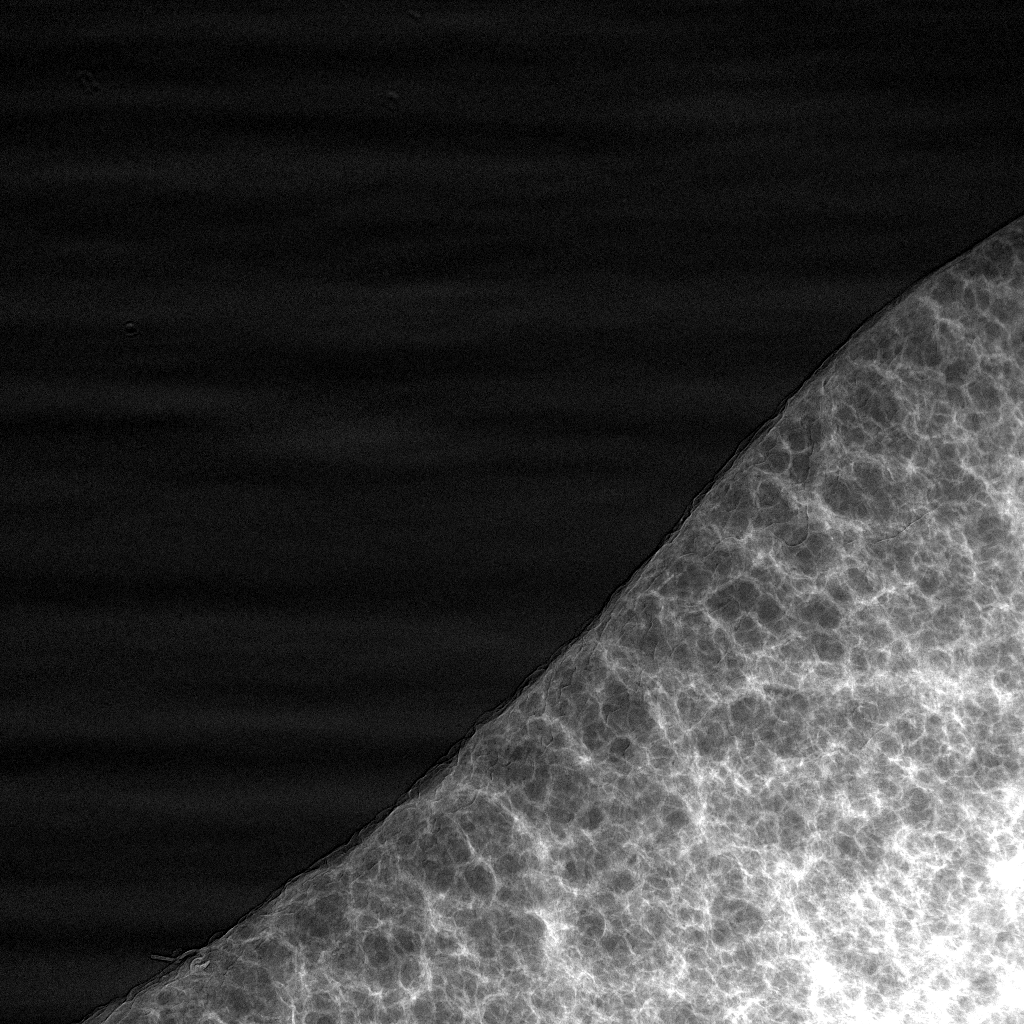
\includegraphics[width=\imagewidth]{img/merge/CP-R108C21Cb_s13358_normalize}};%
%					{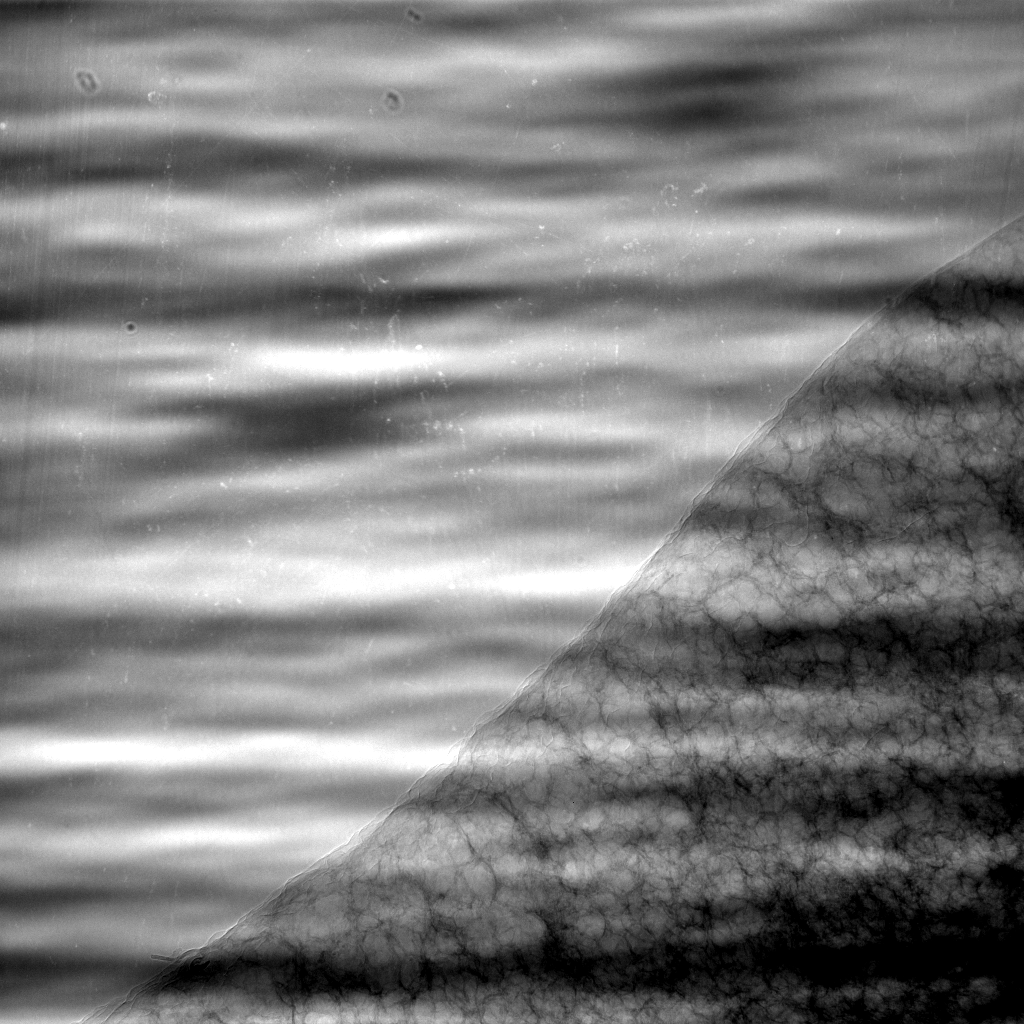
\includegraphics[width=\imagewidth]{R108C21Cb_s13358_normalize}};%
				\def\overlap{141}%
				\fill [red, nearly transparent] (1024-\overlap,1) rectangle (\size,\size);%
				\draw (1024-\overlap,1) rectangle (\size,\size);%
				\node [anchor=south west, color=white] at (0,1024) {(a)};				
			\end{tikzpicture}%
			\begin{tikzpicture}[x=\imagescale,y=-\imagescale]%
				\node[anchor=north west, inner sep=0pt, outer sep=0pt] at (0,0)%
					{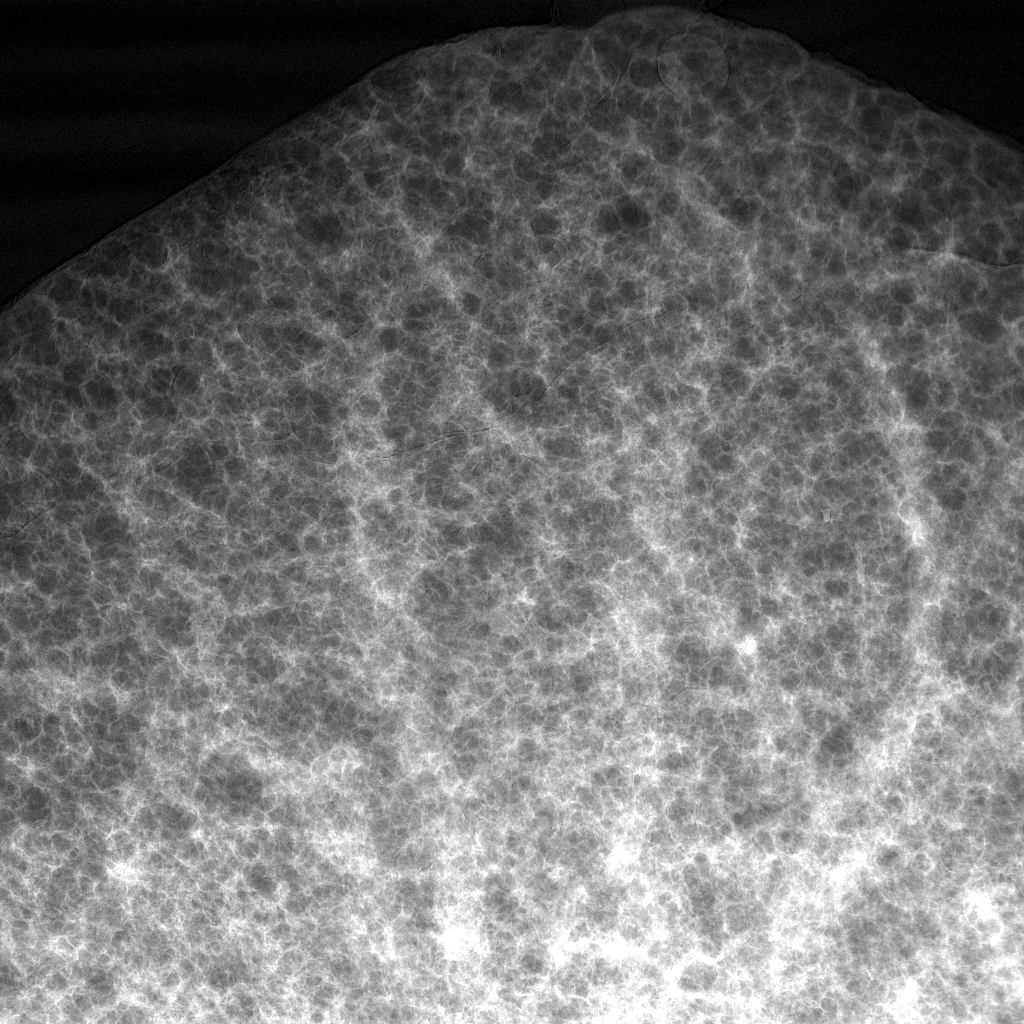
\includegraphics[width=\imagewidth]{img/merge/CP-R108C21Cb_s23358_normalize}};%
%					{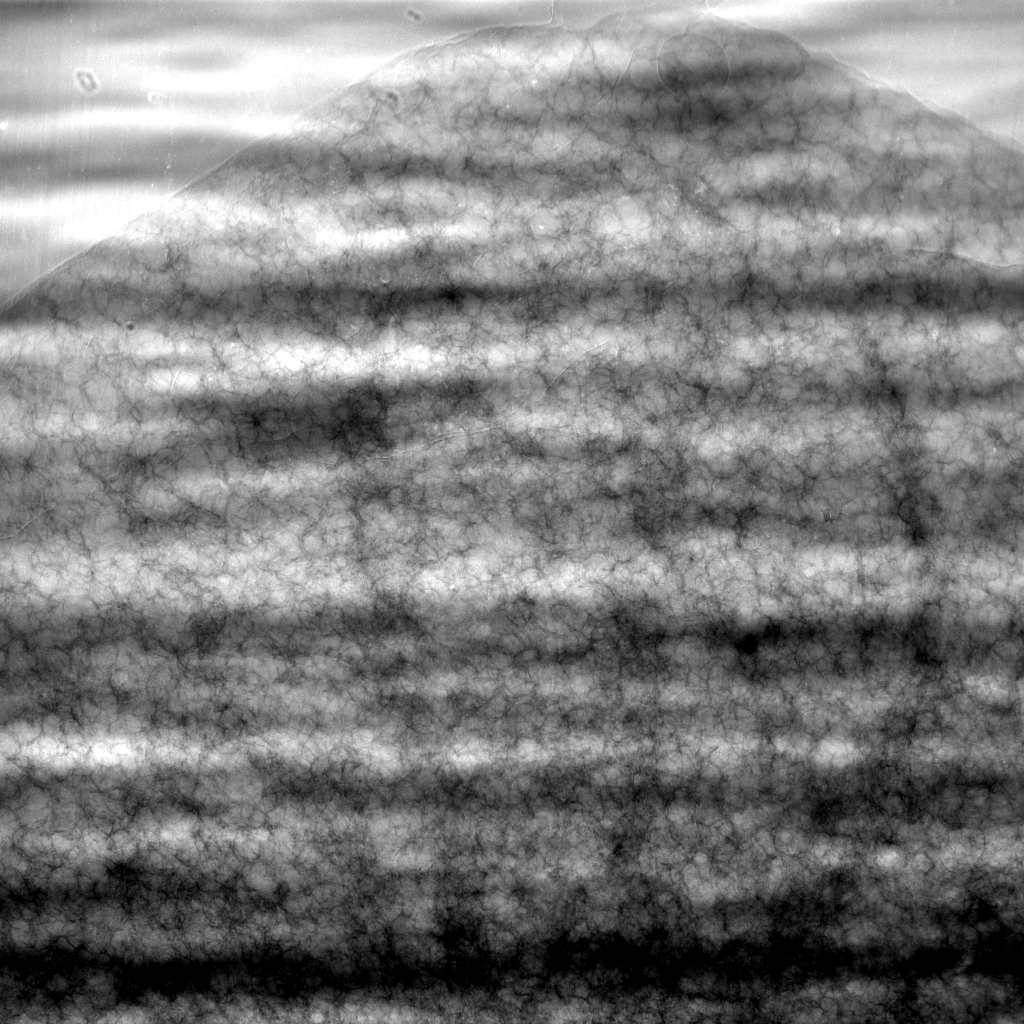
\includegraphics[width=\imagewidth]{R108C21Cb_s23358_normalize}};%
				\def\overlap{141}%
				\fill [green, nearly transparent] (1,1) rectangle (\overlap,\size);%
				\draw (1,1) rectangle (\overlap,\size);%
				\def\overlap{138}%
				\fill [blue, nearly transparent] (1024-\overlap,1) rectangle (\size,\size);%
				\draw (1024-\overlap,1) rectangle (\size,\size);%
			\end{tikzpicture}%
			\begin{tikzpicture}[x=\imagescale,y=-\imagescale]%
				% place image (integer coordinates refer to pixel centers):
				\node[anchor=north west, inner sep=0pt, outer sep=0pt] at (0,0)%
					{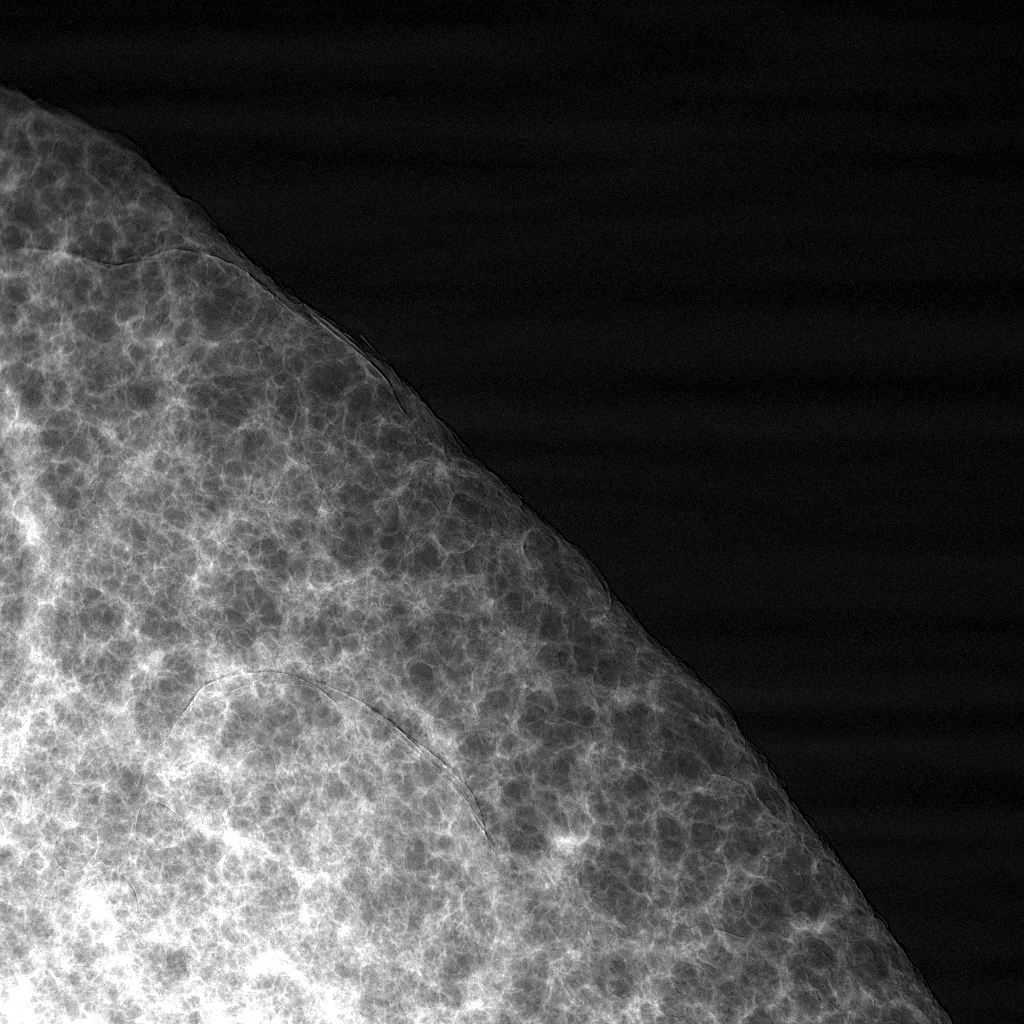
\includegraphics[width=\imagewidth]{img/merge/CP-R108C21Cb_s33358_normalize}};%
%					{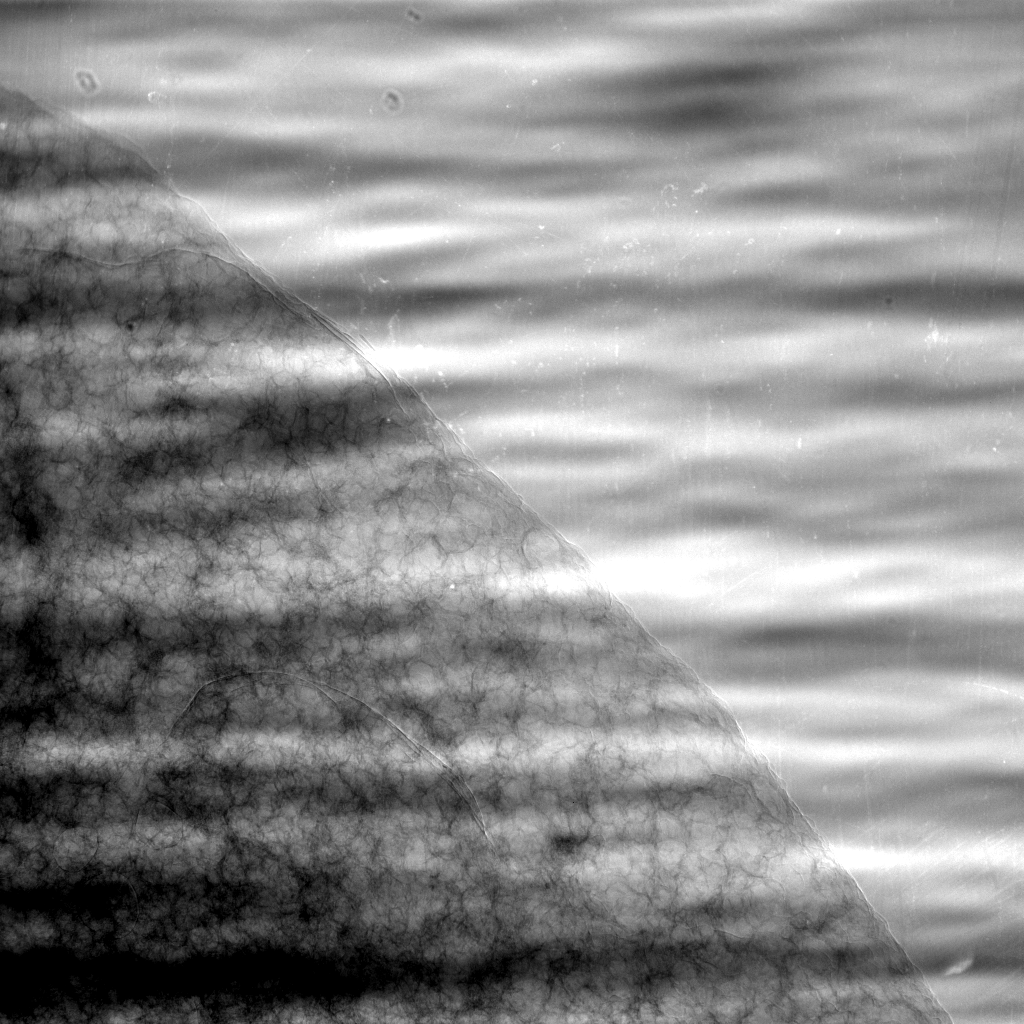
\includegraphics[width=\imagewidth]{R108C21Cb_s33358_normalize}};%
				\def\overlap{138}%
				\fill [yellow, nearly transparent] (1,1) rectangle (\overlap,\size);%
				\draw (1,1) rectangle (\overlap,\size);%
%				\draw[|-|,thick] (5,200) -- (1021,200) node [color=white,midway,above] {\SI{1.51552}{\milli\meter}};%
				\def\x{924}% 1024 - 100
				\def\y{922}% 1024 * .9 = 921.6
				\def\bar{338}% 100 px = 148 um
				\draw[|-|,thick, color=white] (\x-\bar,\y) -- (\x,\y) node [midway, above] {\SI{500}{\micro\meter}};%
			\end{tikzpicture}%
			\label{fig:subscans}%
%%%%%%%%%%%%%%%%%%%%%%%%%%%%%	
%	\caption{caption}
%\end{figure}
%\end{document}\\%
		%\documentclass{article}
%\usepackage{subfig}
%\usepackage{tikz}
%\usepackage{siunitx}
%\begin{document}
%\newcommand{\imsize}{\linewidth}
%\newlength\imagewidth % needed for scalebars
%\newlength\imagescale % needed for scalebars
%\begin{figure}
%	\centering
%%%%%%%%%%%%%%%%%%%%%%%%%%%%%
		\renewcommand{\imsize}{\linewidth}%
		\pgfmathsetlength{\imagewidth}{\imsize} % desired displayed width of image
		\pgfmathsetlength{\imagescale}{\imagewidth/2793}% pixel width of image
			\begin{tikzpicture}[x=\imagescale,y=-\imagescale]%
				\node[anchor=north west,inner sep=0pt,outer sep=0pt] at (0,0)%
					{\includegraphics[width=\imagewidth]{img/merge/R108C21Cb_mrg3333_normalize}};%
%					{\includegraphics[width=\imagewidth]{R108C21Cb_mrg3333_normalize}};%
				\def\x{2693} % 2793-100
				\def\y{922} % 1024*.9 = 921.6
				\def\bar{338} % 100 px = 148 um
				\draw[|-|,thick,color=white] (5,256) -- (2787,256) node [midway,above] {\SI{4.13364}{\milli\meter}};
				\draw[|-|,thick,color=white] (\x-\bar,\y) -- (\x,\y) node [midway,above] {\SI{500}{\micro\meter}};
				\node [anchor=center,color=white] at (100,1024-100) {b)};
				\end{tikzpicture}%
			\label{fig:merge-proj}%
%%%%%%%%%%%%%%%%%%%%%%%%%%%%%	
%	\caption{caption}
%\end{figure}
%\end{document}\\%
		%\documentclass{article}
%\usepackage{subfig}
%\usepackage{tikz}
%\usepackage{siunitx}
%\begin{document}
%\newcommand{\imsize}{\linewidth}
%\newlength\imagewidth % needed for scalebars
%\newlength\imagescale % needed for scalebars
%\begin{figure}
%	\centering
%%%%%%%%%%%%%%%%%%%%%%%%%%%%%
		\pgfmathsetlength{\imagewidth}{\imsize}%
		\pgfmathsetlength{\imagescale}{\imagewidth/2792}%
			\begin{tikzpicture}[x=\imagescale,y=-\imagescale]%
				\node [anchor=north west,inner sep=0pt,outer sep=0pt] at (0,0)%
					{\includegraphics[width=\imagewidth]{img/merge/R108C21Cb_mrg1024rec8bit}};% ``mogrify -shave 0x900 -format png R108C21Cb_mrg1024rec8bit.tif''
%					{\includegraphics[width=\imagewidth]{R108C21Cb_mrg1024rec8bit}};
				\clip (0,0) rectangle (2792,992);				
				\def\x{2692} % 2792-100
				\def\y{893} % 992 * .9 = 892.8
				\def\bar{338} % 100 px = 148 um
				%%%% scalebar
					\draw[|-|,thick,color=white] (\x-\bar,\y) -- (\x,\y) node [midway, above] {\SI{500}{\micro\meter}};
%					\draw[|-|,thick,color=white] (5,30) -- (2787,30) node [midway, below] {\SI{4.13216}{\milli\meter}};
				%%%% center
					\fill [color=red] (2792/2,992/2) circle (5);
				%%%% big circle
					\draw [dashed, ultra thick, color=red] (2792/2,992/2) circle (512);
					\def\angle{35}
					\draw [white, thick, <->] (2792/2,992/2) +(\angle:0) --  node (bigto) {} +(\angle:512); 
					\node [white] (bigfrom) at (349,256){$\frac{1024}{2}$px};
					\draw [white, ->, thick, densely dotted] (bigfrom) to [bend left=45] (bigto);
				%%%% big circle
				%%%% 141px circle
				\draw [dashed, ultra thick, color=red] (2792/2,992/2) circle (512-141);
				\def\angle{35+90}
					\draw [white,thick,<->] (2792/2,992/2) +(\angle:0) -- node (smallto) {} +(\angle:512-141);
					\node [white] (smallfrom) at (349,384) {$\frac{1024}{2}-141$px};
					\draw [white, ->, thick, densely dotted] (smallfrom) to [bend left=45] (smallto);
				%%%% 141px circle					
%				%%%% 138px circle
%				\draw [dashed,color=red] (2792/2,992/2) circle (512-138);
%				\def\angle{45+90+90}
%					\draw [white,<->] (2792/2,992/2) +(\angle:0) -- node (vsmallto) {} +(\angle:512-138);
%					\node [white] (vsmallfrom) at (2972-768,992-512) {$\frac{1024}{2}-138$px};
%					\draw [white,->,densely dotted] (vsmallfrom) to [bend right=45] (vsmallto);
%				%%%% 138px circle
				%%%% inset
%				\newcommand{\size}{.2\imagewidth}%
%				\clip (256,256) rectangle (512,512);
%				\node[anchor=north west,inner sep=0pt,outer sep=0pt] at (0,0)
%					{\includegraphics[width=\size]{R108C21Cb_mrg1024rec8bit}};
%					\draw[white] (0,0) rectangle (\size,-\size);
				%%%% inset
				\node [anchor=south west, color=white] at (0,990) {(c)};			
				\end{tikzpicture}%
			\label{fig:merge-rec}%
%%%%%%%%%%%%%%%%%%%%%%%%%%%%%	
%	\caption{caption}
%\end{figure}
%\end{document}\\%
	\else
	\fi
	\label{fig:wide-field-scan-results}
\end{figure}

Figure~\ref{fig:s2-wfs} clearly shows the advantages provided by the wide field acquisition scheme. With---in this particular case---an enlargement of the field of view by almost a factor of 3, it is possible to visualize several full acini at high resolution. For a conventional scan (fig.~\ref{fig:s2-wfs}(a)), the airway segments in the sample are only partially contained inside the dataset (magenta and yellow). Increasing the field of view (fig.~\ref{fig:s2-wfs}(b)) allows the visualization of those segments to their full extent. A third acinus (cyan) which was not visible in Figure~\ref{fig:s2-wfs}(a) can now easily be visualized.

%\onecolumn
\renewcommand{\imsize}{0.5\linewidth}%
\begin{figure}
	\centering
	\caption{Three-dimensional visualization of the distal-medial tip of the right lower lung lobe of a Sprague Dawley rat. The gray structure in the background shows a semitransparent view of the tomographic dataset with segmented airways. The foreground shows isosurfaces of terminal airways. (a): Conventional scan; the extracted airway segments (magenta and yellow) are only partially contained inside the total sample volume. Airway segments not contained in the dataset, but present in the sample are shown semitransparent. This conventional scan corresponds to a reconstruction of the central of the three wide field scan subscans. (b): Wide field scan with increased field of view; the magenta and yellow segment show multiple full acini inside the dataset, the cyan segment contains a partially cut acinus. All airway segments inside the sample are contained in the tomographic dataset.}
	\ifiucr
	%%%%%%%%%%%%%%%%%%%
		\pgfmathsetlength{\imagewidth}{\imsize}%
		\pgfmathsetlength{\imagescale}{\imagewidth/1379}%
		\begin{tikzpicture}[x=\imagescale,y=-\imagescale]
			\def\x{852} % scalebar-x at golden ratio of x=1379px
			\def\y{898} % scalebar-y at 90% of height of y=998px
			\node[anchor=north west, inner sep=0pt, outer sep=0pt] at (0,0)
				{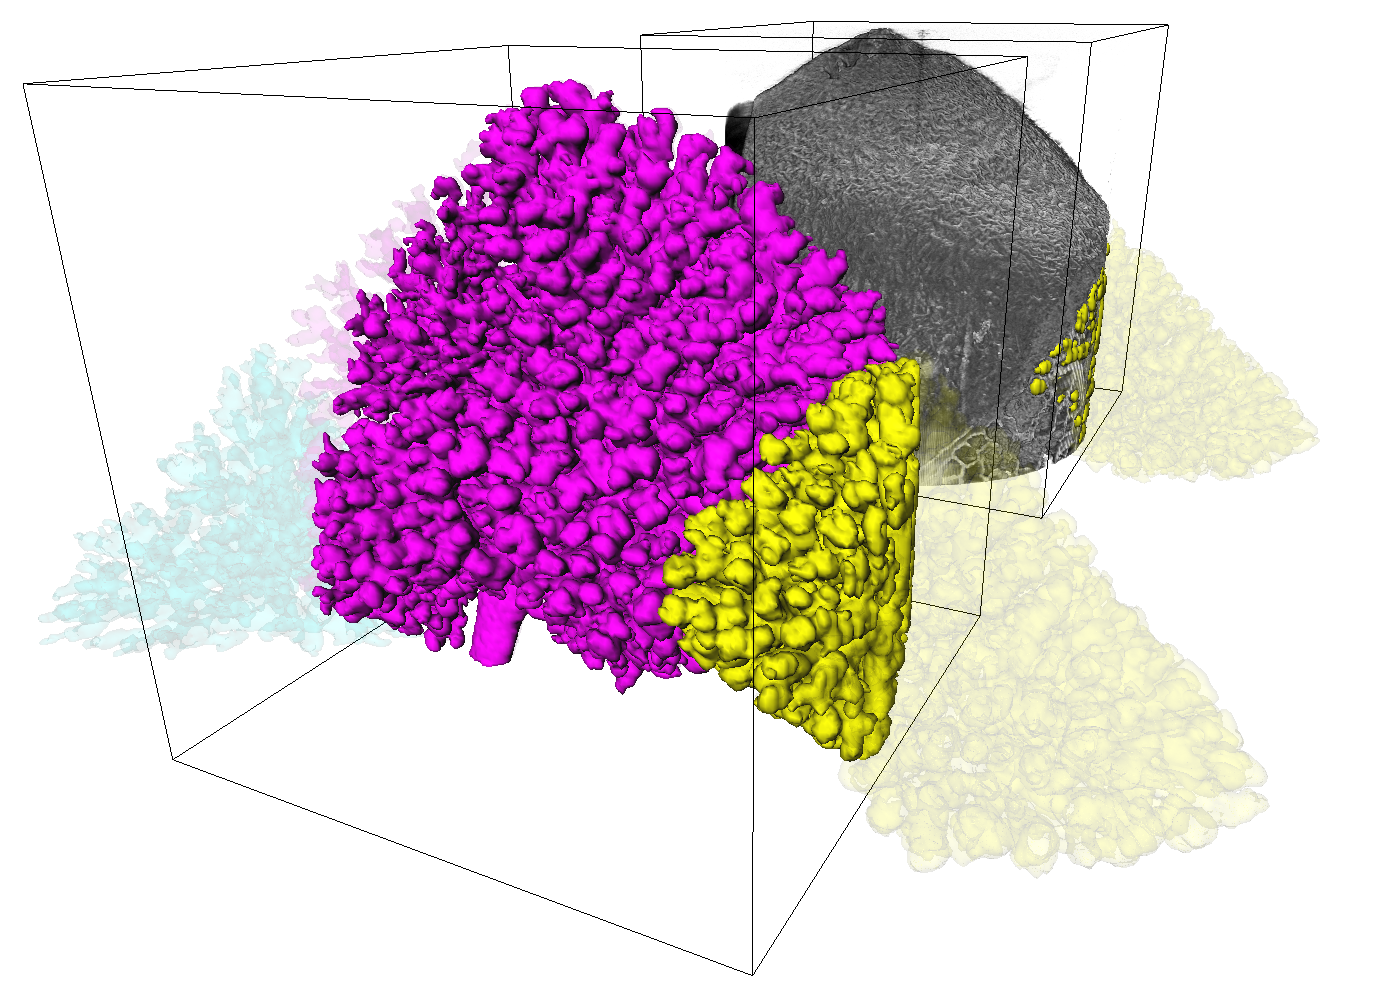
\includegraphics[width=\imagewidth]{img/conv_vs_wfs/scan-conventional}};
			% 618px = 1.5155mm > 100px = 245um > 204px = 500um, 41px = 100um
			\draw[color=red,|-|,thick] (174,761) -- (753,977) node [sloped,midway,above] {\SI{1.5155}{\milli\meter} (1024px)};
			\draw[|-|,thick] (\x,\y) -- (\x+204,\y) node [fill=white, semitransparent, midway, above] {\SI{500}{\micro\meter}};
			\draw[|-|,thick] (\x,\y) -- (\x+204,\y) node [midway, above]{\SI{500}{\micro\meter}};
		\draw[anchor=south west] (0,998) node [fill=white, semitransparent] {(a)} node {(a)};
		\end{tikzpicture}%
	%%%%%%%%%%%%%%%%%%%
		%\\%
		\pgfmathsetlength{\imagewidth}{\imsize}%
		\pgfmathsetlength{\imagescale}{\imagewidth/1379}%
		\begin{tikzpicture}[x=\imagescale,y=-\imagescale]
			\def\x{852} % scalebar-x at golden ratio of x=1379px
			\def\y{898} % scalebar-y at 90% of height of y=998px
			\node[anchor=north west, inner sep=0pt, outer sep=0pt] at (0,0)
				{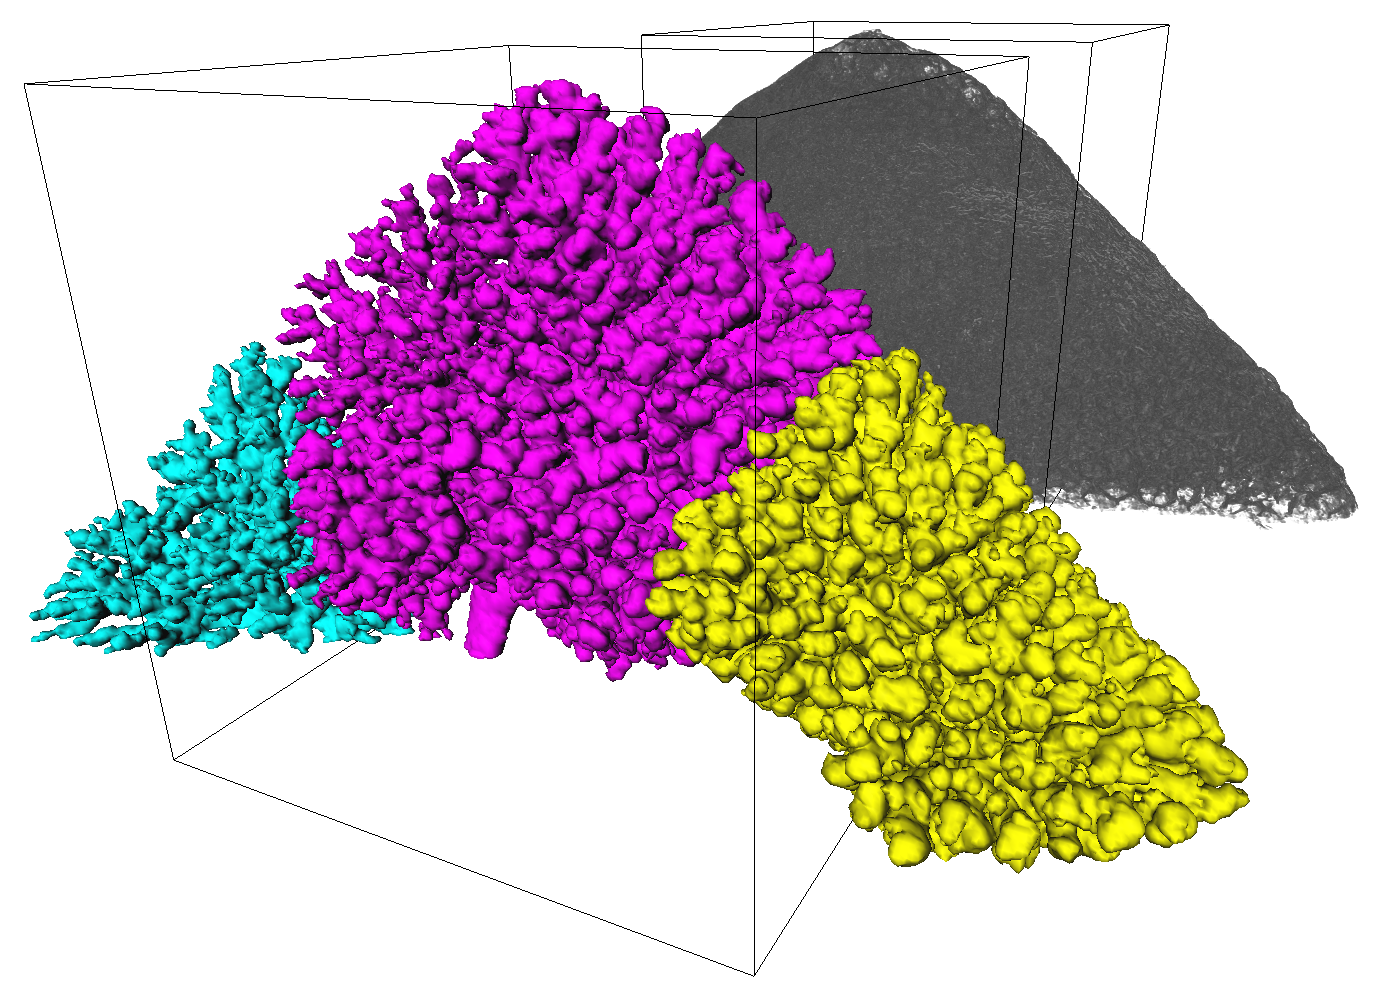
\includegraphics[width=\imagewidth]{img/conv_vs_wfs/scan-widefield}};
			% 620px = 1.5155mm > 100px = 245um > 204px = 500um, 41px = 100um
			\draw[color=red,|-|,thick] (174,761) -- (755,977) node [sloped,midway,above] {\SI{1.5155}{\milli\meter} (1024px)};
			\draw[|-|,thick] (\x,\y) -- (\x+204,\y) node [fill=white, semitransparent, midway, above] {\SI{500}{\micro\meter}};
			\draw[|-|,thick] (\x,\y) -- (\x+204,\y) node [midway, above]{\SI{500}{\micro\meter}};
			\draw[anchor=south west] (0,998) node [fill=white, semitransparent] {(b)} node {(b)};
		\end{tikzpicture}%
	%%%%%%%%%%%%%%%%%%%
	\else
	\fi
	\label{fig:s2-wfs}
\end{figure}
%\twocolumn

As can be seen in Figure~\ref{fig:NormalizedErrorPlot}, the calculated quality of the reconstructions from the different protocols decreases as amount of total obtained projections decreases, as expected. The calculated error of the different protocols, compared to a gold standard protocol (blue diamonds) shows experimental results not derived using simulations with a phantom, but rather real data obtained from actual scans of lung tissue. The plots for the simulation and the normalized difference value are not perfectly in agreement, but show the same trend. The simulation shows an exponential decrease in quality, while the calculated, normalized error shows a more linear decrease in quality from protocol B towards protocol T.

\begin{figure}
	\centering
	\caption{Plot of normalized difference Value ($E_{i_{norm}}$, blue diamonds) for the 19 scanned protocols overlaid over Quality-plot (red dots) obtained from the simulation. The normalized Error has been calculated using the difference image of each protocol $i$ with protocol B. The error bars for each protocol show the standard deviation of the error calculated for 205 of the 1024 slices. Note that the scale of the error was normalized to 20--\SI{100}{\percent}, so that both the quality from the simulation and the error are directly comparable. The abscissa shows the scanning time in percentage of time used for the gold standard scan. Protocol T corresponds to the fastest scanning time, protocol B to the slowest. The protocols in between are shown in decreasing order from T--B for increasing percentage of the scanning time.}
	\ifiucr		
		%\documentclass{article}
%\usepackage{tikz,pgfplots}
%\usepackage[pdftex,active,tightpage]{preview}
%\begin{document}
%\begin{preview}
%%%%%%%%%%%%%%%%%%%%%%%%%%%%%%
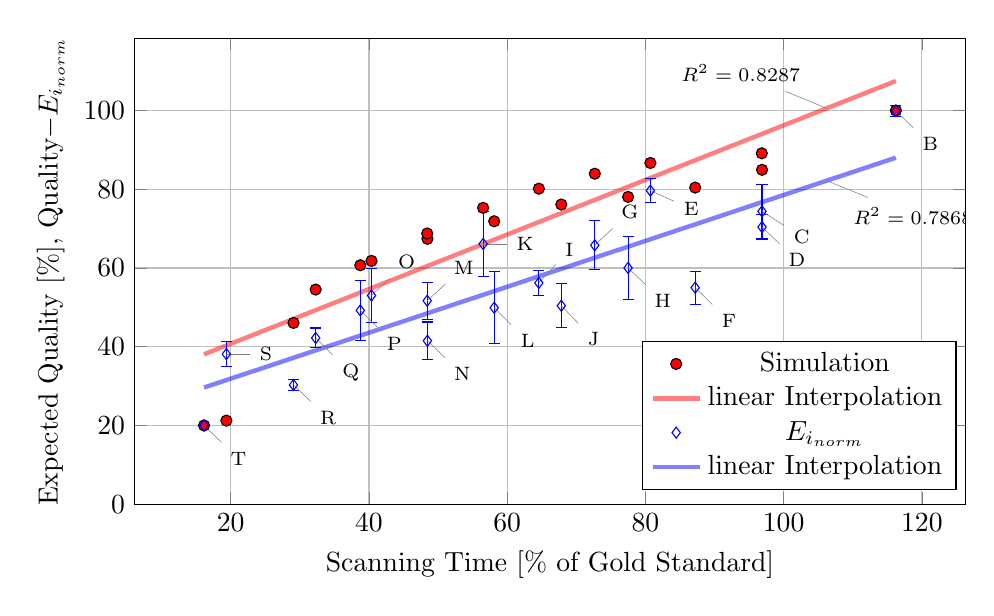
\begin{tikzpicture}

\pgfplotsset{every axis legend/.append style={at={(0.8,0.08)},anchor=base}}

\begin{axis}[%
	xmajorgrids,
  ymajorgrids,
	width=\linewidth,
	height=0.618\linewidth,
	%scale only axis,
	%xmin=0,%xmax=129,
	ymin=0,%ymax=125,
  xlabel={Scanning Time [\%\ of Gold Standard]},%
	ylabel={Expected Quality [\%], Quality$-E_{i_{norm}}$}%
	]

% Protocols
\addplot [ fill=red, only marks, mark = *]
	coordinates{
		(16.14,20)
		(19.37,21.2284)
		(29.08,46.0522)
		(32.29,54.5201)
		(38.75,60.7072)
		(40.37,61.8107)
		(48.46,67.4167)
		(48.43,68.7811)
		(58.12,71.8724)
		(56.52,75.28)
		(67.83,76.1345)
		(64.58,80.1592)
		(77.49,78.0612)
		(72.67,83.9645)
		(87.20,80.4284)
		(80.72,86.6889)
		(96.87,84.9458)
		(96.84,89.1421)
		(116.24,100)
};

\addplot [domain=16.14:116.24,color=red, semitransparent,ultra thick]
	{0.6936*x+26.891}; 

%% Line plot
%\addplot [smooth, solid, semitransparent]
	%coordinates{
		%(16.14,16.8548)
		%(19.37,25.9575)
		%(29.08,46.6567)
		%(32.29,51.7347)
		%(38.75,59.9714)
		%(40.37,61.6854) 
		%(48.46,68.6146)
		%(48.43,68.6305) 
		%(56.52,73.5452)
		%(58.12,74.3455)
		%(64.58,77.1605)
		%(67.83,78.3754)
		%(72.67,80.0091)
		%(77.49,81.5005)
		%(80.72,82.4599)
		%(87.20,84.3973)
		%(96.87,87.719)
%%		(96.87,87.719)
		%(116.24,99.8565)
%};

\addplot [ color=blue, only marks, mark=diamond ]
plot [ error bars/.cd, y dir=both, y explicit ]
    coordinates{
	( 16.14,20.0000) +- (0,0)      % T
	( 19.37,38.1358) +- (0,3.1135) % S
	( 29.08,30.2919) +- (0,1.3958) % R
	( 32.29,42.2255) +- (0,2.5278) % Q
	( 38.75,49.2247) +- (0,7.6789) % P
	( 40.37,53.0181) +- (0,6.8507) % O 
	( 48.46,41.5079) +- (0,4.7824) % N  
	( 48.43,51.6990) +- (0,4.7110) % M
	( 58.12,49.9058) +- (0,9.1839) % L
	( 56.52,66.1100) +- (0,8.1635) % K
	( 67.83,50.4137) +- (0,5.5671) % J
	( 64.58,56.2138) +- (0,3.2329) % I
	( 77.49,60.0243) +- (0,8.0805) % H
	( 72.67,65.7727) +- (0,6.2214) % G
	( 87.20,55.0069) +- (0,4.1882) % F
	( 80.72,79.6708) +- (0,3.0107) % E
	( 96.87,70.4018) +- (0,3.0863) % D
	( 96.87,74.3991) +- (0,6.8125) % C
	(116.24,99.8987) +- (0,1.3487) % B
};

\addplot [domain=16.14:116.24,color=blue, semitransparent,ultra thick]
	{0.5833*x+20.226}; 

\legend{%
	Simulation,%
	linear Interpolation,%
	$E_{i_{norm}}$,%
	linear Interpolation}

% \draw [<-] (axis cs:97.87,74.3991) -- (axis cs:99.87,74.3991) node [anchor=text] {\tiny C}; 
% \draw [<-] (axis cs:97.87,70.4018) -- (axis cs:99.87,70.4018) node [anchor=text] {\tiny D};
% \draw [<-] (axis cs:81.72,79.6708) -- (axis cs:82.72,79.6708) node [anchor=text] {\tiny E};
% \draw [<-] (axis cs:78.49,60.0243) -- (axis cs:79.49,60.0243) node [anchor=text] {\tiny H};
% \draw [<-] (axis cs:65.58,56.2138) -- (axis cs:66.58,56.2138) node [anchor=text] {\tiny I};
% \draw [<-] (axis cs:49.43,51.6990) -- (axis cs:51.43,51.6990) node [anchor=text] {\tiny M};
% \draw [<-] (axis cs:49.46,41.5079) -- (axis cs:51.46,41.5079) node [anchor=text] {\tiny N};

\tikzstyle{every pin}=[pin distance=2ex,font=\scriptsize]
\node[coordinate, pin=below right:{B}] at (axis cs:116.24,99.8987) {}; % B
\node[coordinate, pin=-22.5:{C}] at (axis cs:96.87,74.3991) {}; % C
\node[coordinate, pin=below right:{D}] at (axis cs:96.87,70.4018) {}; % D
\node[coordinate, pin=-5:{E}] at (axis cs:80.72,79.6708) {}; % E
\node[coordinate, pin=below right:{F}] at (axis cs:87.20,55.0069) {}; % F
\node[coordinate, pin=above right:{G}] at (axis cs:72.67,65.7727) {}; % G
\node[coordinate, pin=below right:{H}] at (axis cs:77.49,60.0243) {}; % H
\node[coordinate, pin=above right:{I}] at (axis cs:64.58,56.2138) {}; % I
\node[coordinate, pin=below right:{J}] at (axis cs:67.83,50.4137) {}; % J
\node[coordinate, pin=right:{K}] at (axis cs:56.52,66.1100) {}; % K
\node[coordinate, pin=below right:{L}] at (axis cs:58.12,49.9058) {}; % L
\node[coordinate, pin=above right:{M}] at (axis cs:48.43,51.6990) {}; % M
\node[coordinate, pin=below right:{N}] at (axis cs:48.46,41.5079) {}; % N  
\node[coordinate, pin=above right:{O}] at (axis cs:40.37,53.0181) {}; % O
\node[coordinate, pin=below right:{P}] at (axis cs:38.75,49.2247) {}; % P
\node[coordinate, pin=below right:{Q}] at (axis cs:32.29,42.2255) {}; % Q
\node[coordinate, pin=below right:{R}] at (axis cs:29.08,30.2919) {}; % R
\node[coordinate, pin=right:{S}] at (axis cs:19.37,38.1358) {}; % S
\node[coordinate, pin=below right:{T}] at (axis cs:16.14,20.0000) {}; % T

\node[coordinate, pin=above left:{$R^2=0.8287$}] at (axis cs:106.24,100.5791) {};
\node[coordinate, pin=below right:{$R^2=0.7868$}] at (axis cs:106.24, 82.1958) {};


\end{axis}

\end{tikzpicture}
%%%%%%%%%%%%%%%%%%%%%%%%%%%%%%
%\end{preview}
%\end{document}

%%%%%%%%%%%%%%%%%%%%%%%%%%%%%%
% plot erstellt mit MATLAB-File p:\\MATLAB\WideFieldScan/Paper/wfs_Compare2008c_ErrorPlot.m
% mit FromToTo = 1:5:1024
% sowie matlab2tikz
% Daten
%%%%%%%%%%Time =
%%%%%%%%%%  Columns 1 through 12
%%%%%%%%%%
%%%%%%%%%%   13.75   16.50   24.77   27.50   33   34.38   41.27   41.25   49.50   48.14   57.77   55
%%%%%%%%%%
%%%%%%%%%%  Columns 13 through 19
%%%%%%%%%%
%%%%%%%%%%   66   61.89   74.27   68.75   82.50   82.50   99.01
%MeanCumulativeError =
%
%  Columns 1 through 12
%
%   20.0000   38.1358   30.2919   42.2255   49.2247   53.0181   41.5079   51.6990   49.9058   66.1100   50.4137   56.2138
%
%  Columns 13 through 19
%
%   60.0243   65.7727   55.0069   79.6708   70.4018   74.3991   99.8987
%
%
%StandardDeviationofCumulativeError =
%
%  Columns 1 through 12
%
%         0    3.1135    1.3958    2.5278    7.6789    6.8507    4.7824    4.7110    9.1839    8.1635    5.5671    3.2329
%
%  Columns 13 through 19
%
%    8.0805    6.2214    4.1882    3.0107    3.0863    6.8125    1.3487
%%%%%%%%%%%%%%%%%%%%%%%%%%%%%%
	\else
	\fi
	\label{fig:NormalizedErrorPlot}
\end{figure}

\subsubsection{Three-dimensional visualization of different protocols}
\label{subsec:comparison}
The tomograms of the different protocols were three-dimensionally analyzed and visualized using MeVisLab (Version 2.0 (2009-06-09 Release), MeVis Medical Solutions AG and Fraunhofer MEVIS - Institute for Medical Image Computing, Bremen, Germany). Airway segments were extracted using a threshold interval based region growing algorithm~\cite{Zucker1976}. A seed point for the region growing algorithm was manually defined in the most proximal slice for each independent airway segment. The coordinates of the seed points were kept constant for protocol B--T, allowing direct comparison between the airway segment reconstructions of the different protocols. Airway segments extracted for protocol B, L and T are shown in Figure~\ref{fig:BvsT}.

The three-dimensional isosurface visualizations shown in Figure~\ref{fig:BvsT} represent three of the 19 scanned protocols. Protocol B corresponds to a slightly oversampled gold standard scan, obtained with total 15732 projections, recorded in \SI{66}{\minute}. Protocol L was obtained in \SI{35}{\minute} with total 7866 projections. Protocol T was obtained in \SI{12}{\minute} with 2185 projections for all three subscans. The tomographic dataset from protocol B was reconstructed from 5244 merged projection images, the dataset from protocol L was reconstructed from 2622 merged projections and the dataset from protocol T was reconstructed using only 874 merged projections. Even though protocols L and T were scanned while violating the sampling theorem and with a total scanning time reduction of \SI{40}{\percent} (L) or more than \SI{86}{\percent} (T), the samples still appear to be identical to the gold standard protocol in the low-resolution three-dimensional visualizations shown in Figure~\ref{fig:BvsT}(a)--(c).

Figure~\ref{fig:BvsT}(d)--(f) show isosurface visualizations of the border between airspace and lung tissue as cubic regions of interest (256 pixels wide, marked blue in Figure~\ref{fig:BvsT}(a)--(c)). Because of experimental constraints, the cutline between the individual subscans could not be defined with a precision of one single pixel. As a consequence, the clipping plane does not lie in exactly the same position. This explains the appearing and disappearing holes in Figure~\ref{fig:BvsT}(d)--(f).

Even with the higher magnification, the reconstruction of protocol L in Figure~\ref{fig:BvsT}(e) appears nearly identical to the reconstruction of the region of interest of protocol B (fig.~\ref{fig:BvsT}(d)). The isosurface of the region of interest of protocol T shown in Figure~\ref{fig:BvsT}(f) appears rougher than the isosurface of protocol B. This roughness is introduced through ray-like artifacts visible in the original slice of the dataset of protocol T (not shown). These artifacts are the consequence of a strong subsampling. With the acquisition of only 874 projections instead of the required 5139, the sampling theorem is far from being satisfied. However, even with this strong undersampling, segmentation, three-dimensional reconstruction and visualization of the sample is still possible.

%\onecolumn
\renewcommand{\imsize}{.33\linewidth}%
\begin{figure}
	\centering
	\caption{Comparison of three-dimensional visualizations. %
			(a)--(c): Three independent airway segments (cyan, magenta, yellow) of tomographic datasets obtained with protocol B, L and T, extracted using a region growing algorithm. A cubic region of interest (blue) with a side length of 256 pixels (corresponding to \SI{379}{\micro\meter}) is marked inside the leftmost segment for all protocols. %
			(d)--(f): Detailed view of isosurfaces of the lung tissue inside the blue ROIs for protocol B, L and T, respectively. Note the increasing surface roughness in the alveolar surfaces for subfigures (e) and (f).}%
	\ifiucr			
		\pgfmathsetlength{\imagewidth}{\imsize}%
		\pgfmathsetlength{\imagescale}{\imagewidth/1770}%
		\def\x{1094} % scalebar-x at golden ratio of x=1770px
		\def\y{853} % scalebar-y at 90% of height of y=948px
	%%%%%%%%%%%%%%%
		\begin{tikzpicture}[x=\imagescale,y=-\imagescale]
			\node[anchor=north west, inner sep=0pt, outer sep=0pt] at (0,0) {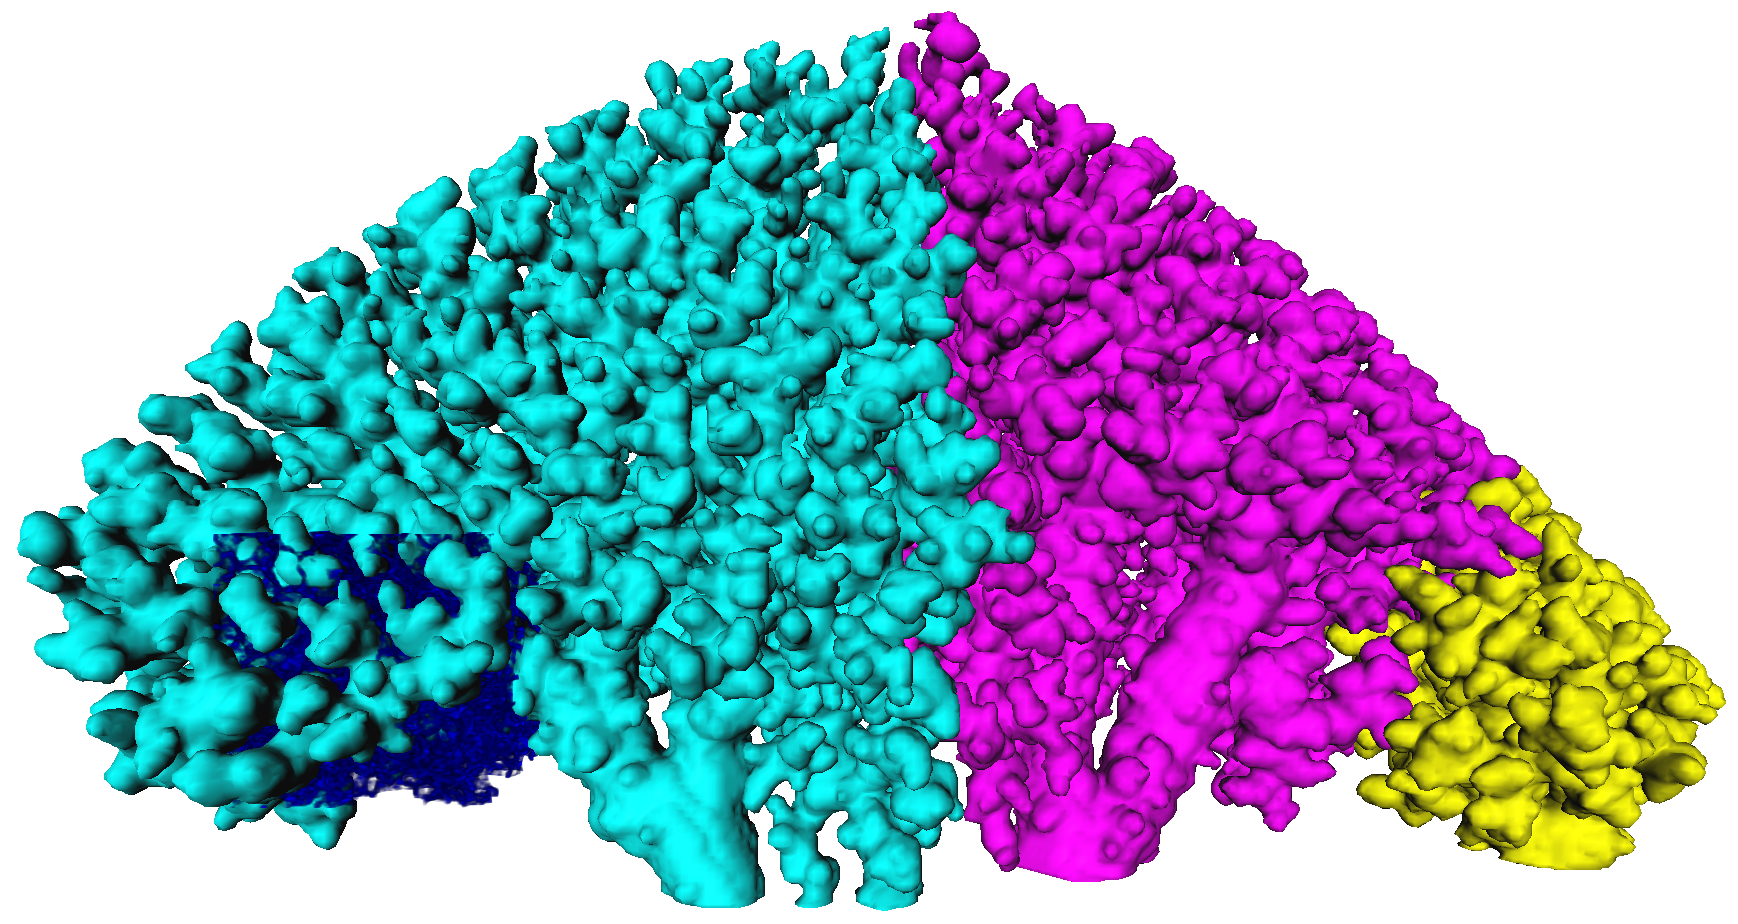
\includegraphics[width=\imagewidth]{img/comparisonBvsT/ob}};
			% 1415px = 1.9568mm > 100px = 138um > 361px = 500um, 72px = 100um
			% \draw[|-|,thick] (340,864) -- (1747,717) node [sloped,midway,above] {\SI{1.9568}{\milli\meter} (1322.171px)};
			\draw[|-|,thick] (\x,\y) -- (\x+361,\y) node [fill=white, semitransparent, midway, above] {\SI{500}{\micro\meter}};
			\draw[|-|,thick] (\x,\y) -- (\x+361,\y) node [midway, above]{\SI{500}{\micro\meter}};
			\draw[anchor=south west] (0,948) node [fill=white, semitransparent] {(a)} node {(a)};
		\end{tikzpicture}%
	%%%%%%%%%%%%%%%
		\begin{tikzpicture}[x=\imagescale,y=-\imagescale]
			\node[anchor=north west, inner sep=0pt, outer sep=0pt] at (0,0) {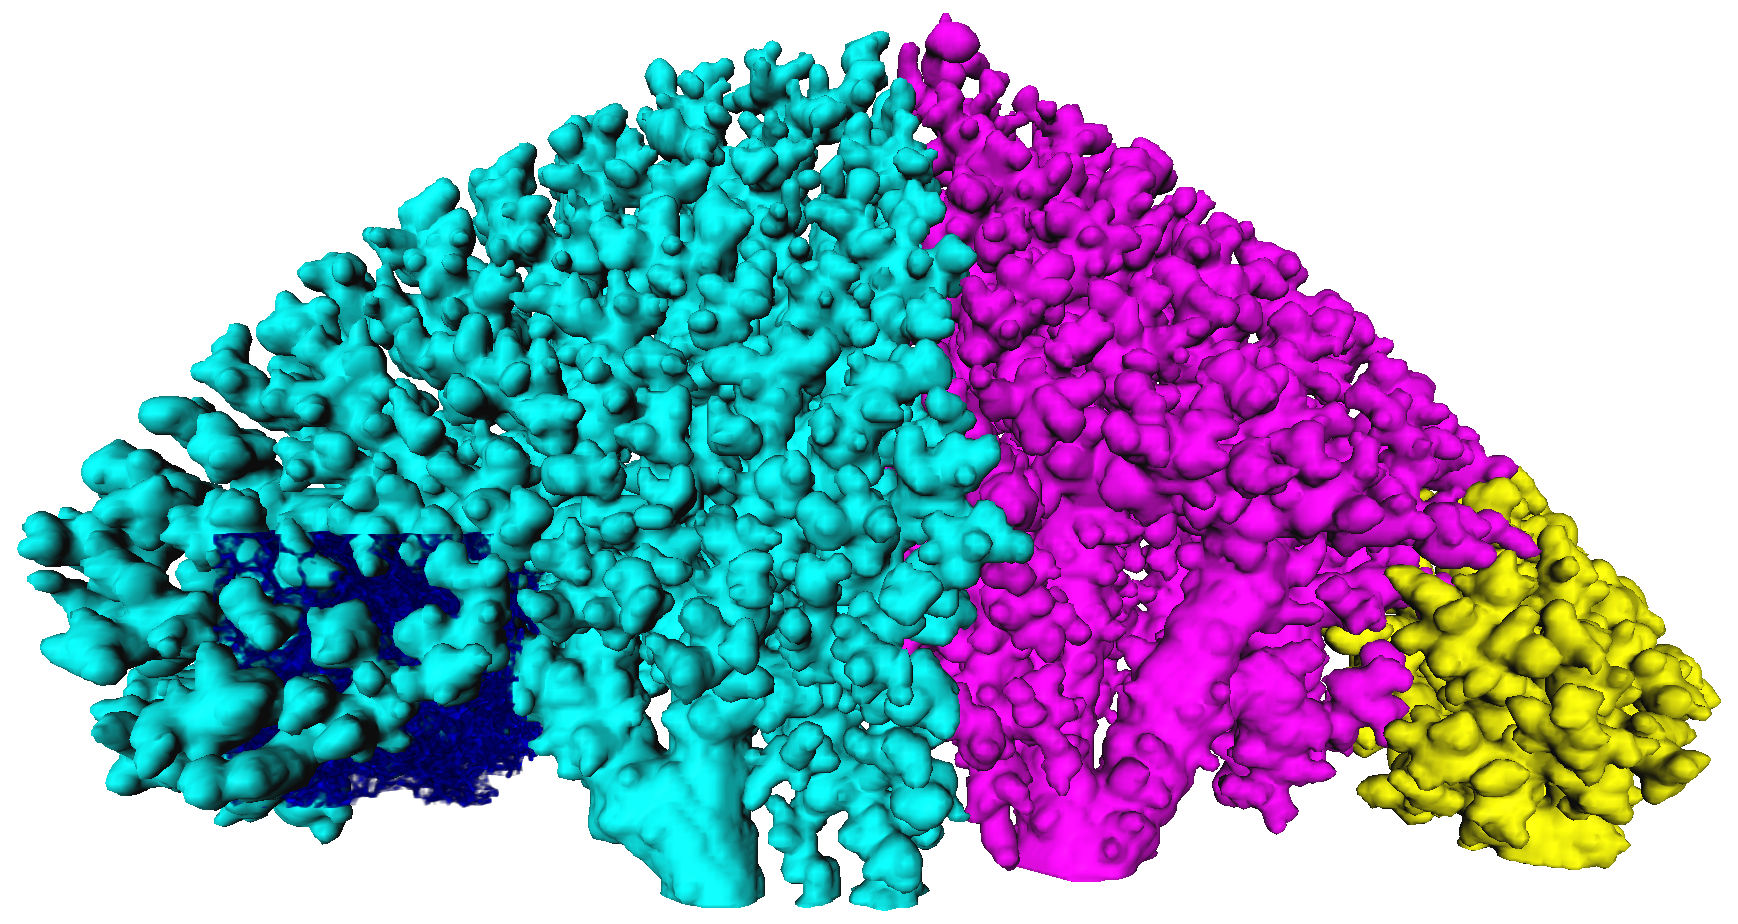
\includegraphics[width=\imagewidth]{img/comparisonBvsT/ol}};
			% 1415px = 1.9568mm > 100px = 138um > 361px = 500um, 72px = 100um
			% \draw[|-|,thick] (340,864) -- (1747,717) node [sloped,midway,above] {\SI{1.9568}{\milli\meter} (1322.171px)};
			\draw[|-|,thick] (\x,\y) -- (\x+361,\y) node [fill=white, semitransparent, midway, above] {\SI{500}{\micro\meter}};
			\draw[|-|,thick] (\x,\y) -- (\x+361,\y) node [midway, above]{\SI{500}{\micro\meter}};
			\draw[anchor=south west] (0,948) node [fill=white, semitransparent] {(b)} node {(b)};
		\end{tikzpicture}%
	%%%%%%%%%%%%%%%
		\begin{tikzpicture}[x=\imagescale,y=-\imagescale]
			\node[anchor=north west, inner sep=0pt, outer sep=0pt] at (0,0) {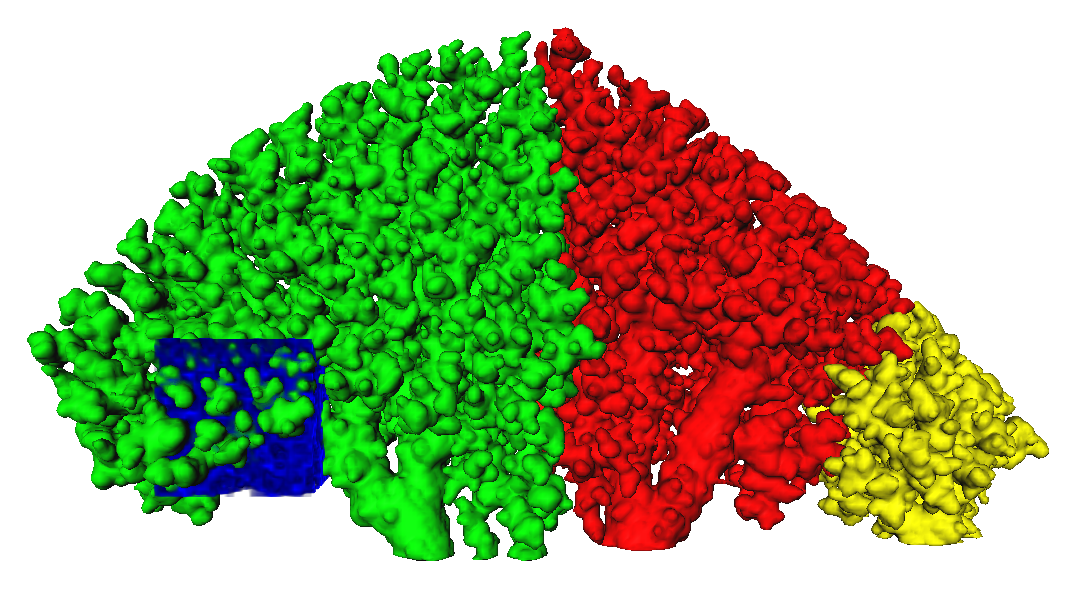
\includegraphics[width=\imagewidth]{img/comparisonBvsT/ot}};
			% 1415px = 1.9568mm > 100px = 138um > 361px = 500um, 72px = 100um
			% \draw[|-|,thick] (340,864) -- (1747,717) node [sloped,midway,above] {\SI{1.9568}{\milli\meter} (1322.171px)};
			\draw[|-|,thick] (\x,\y) -- (\x+361,\y) node [fill=white, semitransparent, midway, above] {\SI{500}{\micro\meter}};
			\draw[|-|,thick] (\x,\y) -- (\x+361,\y) node [midway, above]{\SI{500}{\micro\meter}};
			\draw[anchor=south west] (0,948) node [fill=white, semitransparent] {(c)} node {(c)};
		\end{tikzpicture}%
	%%%%%%%%%%%%%%%
		\\%
		\pgfmathsetlength{\imagewidth}{\imsize}%
		\pgfmathsetlength{\imagescale}{\imagewidth/799}%
		\def\x{494} % scalebar-x at golden ratio of x=799px
		\def\y{720} % scalebar-y at 90% of height of y=800px
	%%%%%%%%%%%%%%%
		\begin{tikzpicture}[x=\imagescale,y=-\imagescale]
			\node[anchor=north west, inner sep=0pt, outer sep=0pt] at (0,0) {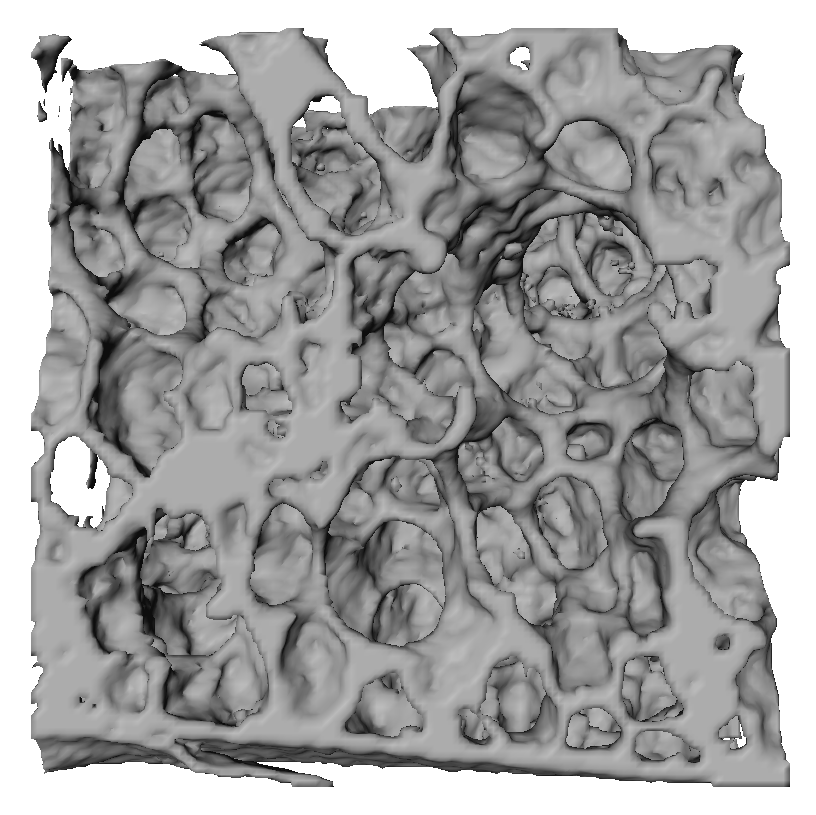
\includegraphics[width=\imagewidth]{img/comparisonBvsT/roiB}};
			% 758px = 0.37888mm > 100px = 50um > 1000px = 500um, 200px = 100um
			% \draw[|-|,thick] (20,138) -- (778,136) node [sloped,midway,above] {\SI{0.37888}{\milli\meter} (256px)};
			\draw[|-|,thick] (\x,\y) -- (\x+100,\y) node [fill=white, semitransparent, midway, above] {\SI{50}{\micro\meter}};
			\draw[|-|,thick] (\x,\y) -- (\x+100,\y) node [midway, above]{\SI{50}{\micro\meter}};
			\draw[anchor=south west] (0,800) node [fill=white, semitransparent] {(d)} node {(d)};
		\end{tikzpicture}%
	%%%%%%%%%%%%%%%
		\begin{tikzpicture}[x=\imagescale,y=-\imagescale]
			\node[anchor=north west, inner sep=0pt, outer sep=0pt] at (0,0) {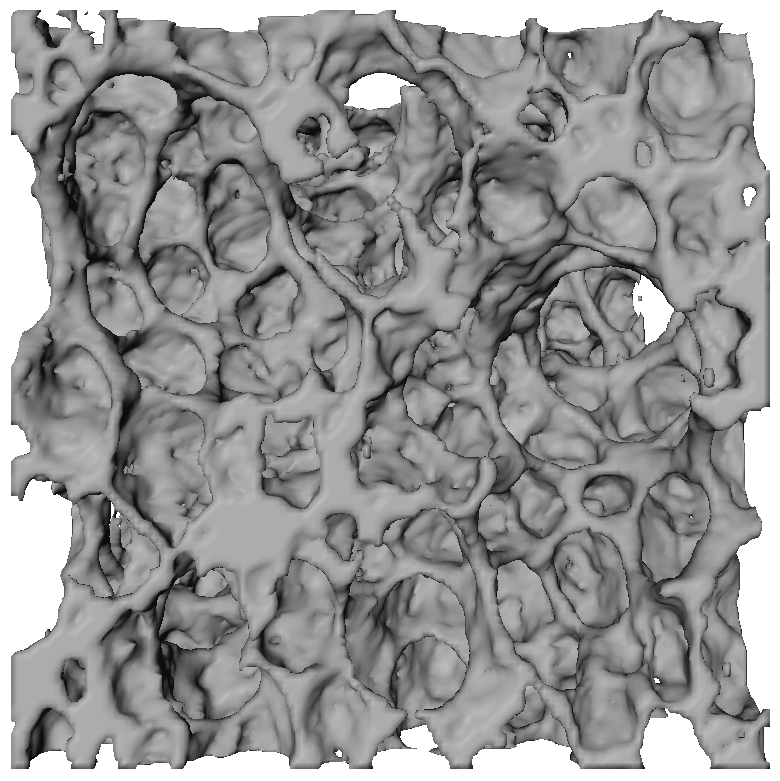
\includegraphics[width=\imagewidth]{img/comparisonBvsT/roiL}};
			% 758px = 0.37888mm > 100px = 50um > 1000px = 500um, 200px = 100um
			% \draw[|-|,thick] (20,138) -- (778,136) node [sloped,midway,above] {\SI{0.37888}{\milli\meter} (256px)};
			\draw[|-|,thick] (\x,\y) -- (\x+100,\y) node [fill=white, semitransparent, midway, above] {\SI{50}{\micro\meter}};
			\draw[|-|,thick] (\x,\y) -- (\x+100,\y) node [midway, above]{\SI{50}{\micro\meter}};
			\draw[anchor=south west] (0,800) node [fill=white, semitransparent] {(e)} node {(e)};
		\end{tikzpicture}%
	%%%%%%%%%%%%%%%
		\begin{tikzpicture}[x=\imagescale,y=-\imagescale]
			\node[anchor=north west, inner sep=0pt, outer sep=0pt] at (0,0) {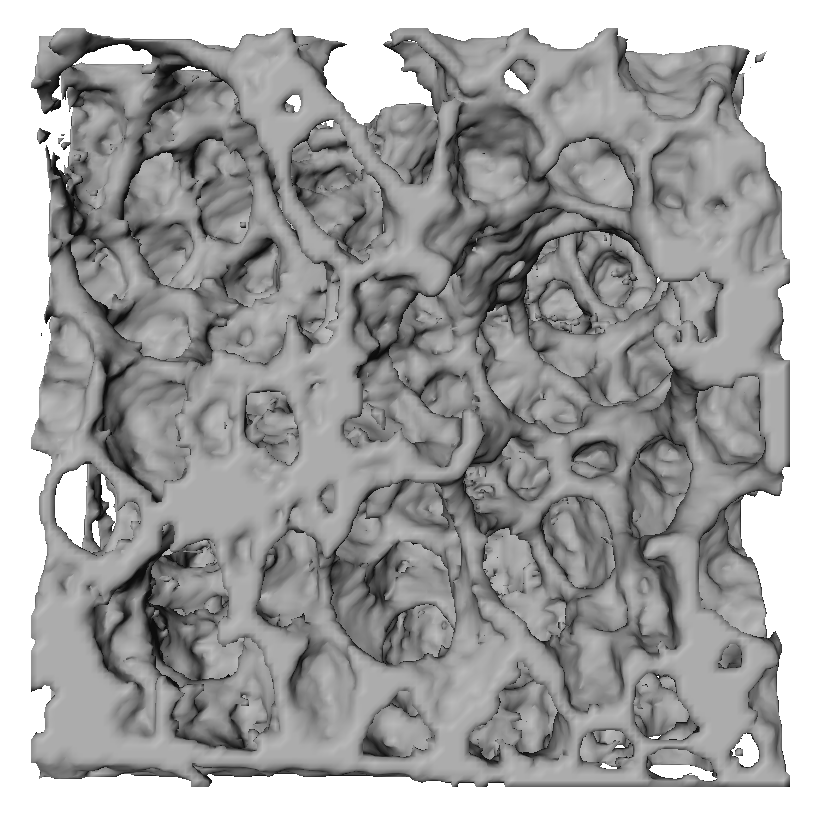
\includegraphics[width=\imagewidth]{img/comparisonBvsT/roiT}};
			% 758px = 0.37888mm > 100px = 50um > 1000px = 500um, 200px = 100um
			% \draw[|-|,thick] (20,138) -- (778,136) node [sloped,midway,above] {\SI{0.37888}{\milli\meter} (256px)};
			\draw[|-|,thick] (\x,\y) -- (\x+100,\y) node [fill=white, semitransparent, midway, above] {\SI{50}{\micro\meter}};
			\draw[|-|,thick] (\x,\y) -- (\x+100,\y) node [midway, above]{\SI{50}{\micro\meter}};
			\draw[anchor=south west] (0,800) node [fill=white, semitransparent] {(f)} node {(f)};
		\end{tikzpicture}%
	%%%%%%%%%%%%%%%
	\else
	\fi
	\label{fig:BvsT}
\end{figure}%
%\twocolumn%

For further analysis four regions of interest with a side length of 256 pixels (at \SI{1.48}{\micro\meter\per pixel}) have been extracted for each of the protocols B, L and T. The three-dimensional placement of these ROIs inside the sample is shown in Figure~\ref{fig:roi3d}.

\renewcommand{\imsize}{\columnwidth}
\begin{figure}
	\centering
	\caption{Overview of the placement of the four regions of interest where the histogram of the euclidean distance transformation distribution has been calculated. Grey: Semitransparent volume rendering of the lung tissue sample. Red: Four regions of interest, extracted to calculate the distance transformation. The labels of the ROIs conform to the legends in Figure~\ref{fig:DTFplots}.}%
	\ifiucr
		\pgfmathsetlength{\imagewidth}{\imsize}%
		\pgfmathsetlength{\imagescale}{\imagewidth/1563}%
		\begin{tikzpicture}[x=\imagescale,y=-\imagescale]
			\def\x{966} % scalebar-x at golden ratio of x=1563px
			\def\y{768} % scalebar-y at 90% of height of y=853px
			\node[anchor=north west, inner sep=0pt, outer sep=0pt] at (0,0) {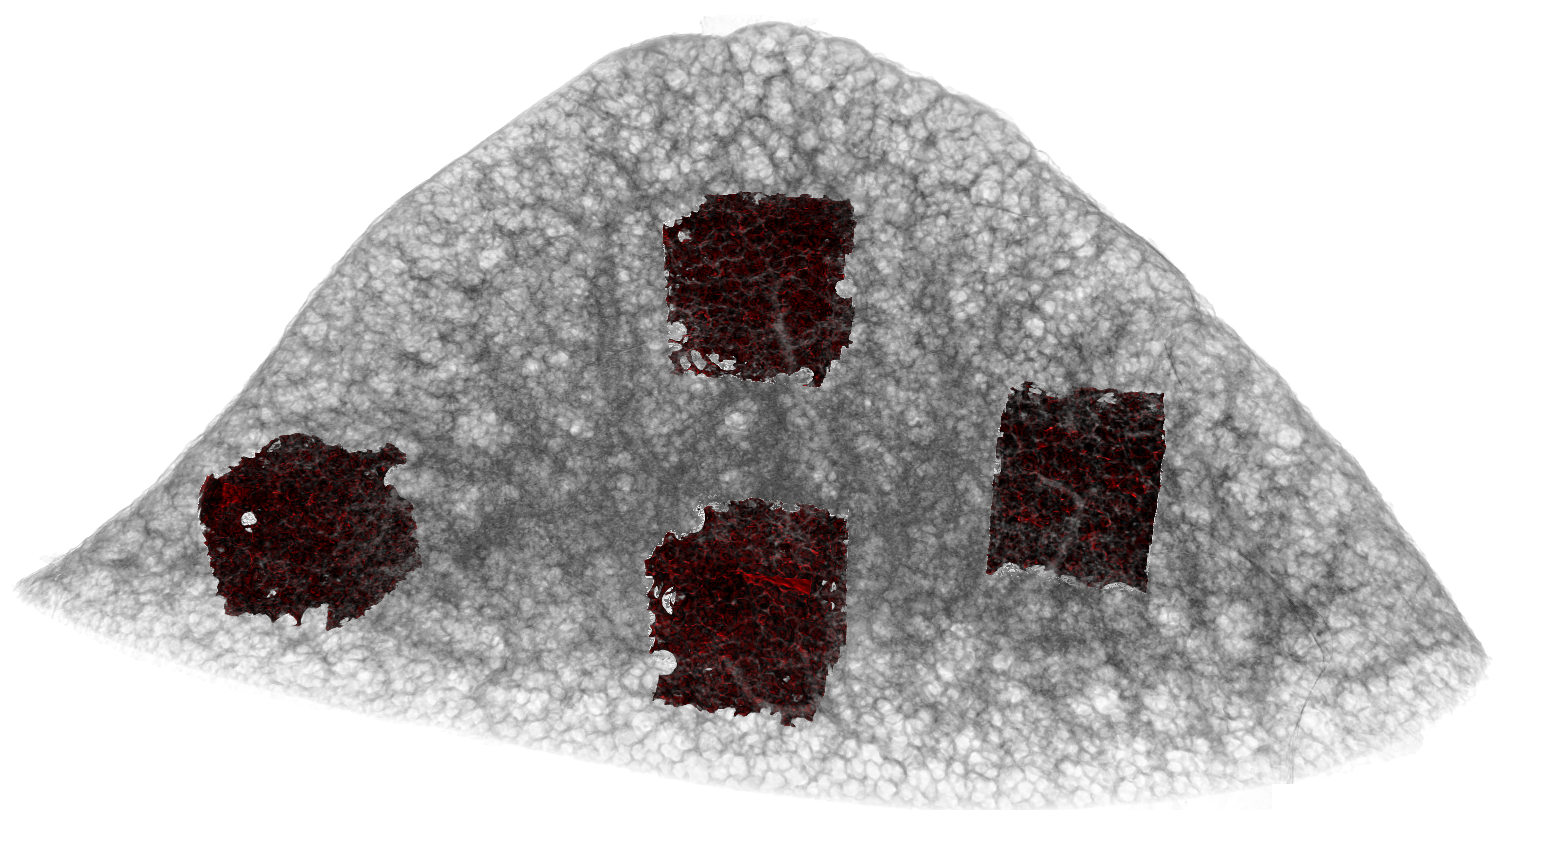
\includegraphics[width=\imagewidth]{img/dtf-roi/ROIs-3d}};
			% 1551px = 4.0138mm > 100px = 259um > 193px = 500um, 39px = 100um
			\draw[|-|,thick] (\x,\y) -- (\x+193,\y) node [fill=white, semitransparent, midway, above] {\SI{500}{\micro\meter}};
			\draw[|-|,thick] (\x,\y) -- (\x+193,\y) node [midway, above] {\SI{500}{\micro\meter}};
			\draw ( 300,400) node [fill=white, semitransparent] {ROI 1} node {ROI 1}; % 523-497-743
			\draw ( 740,460) node [fill=white, semitransparent] {ROI 2} node {ROI 2}; % 1382-546-743
			\draw ( 760,160) node [fill=white, semitransparent] {ROI 3} node {ROI 3}; % 1324-266-289
			\draw (1080,350) node [fill=white, semitransparent] {ROI 4} node {ROI 4}; % 1863-237-604
		\end{tikzpicture}%
	\else
	\fi		
	\label{fig:roi3d}
\end{figure}

Each of the ROIs has been binarized using an algorithmically determined threshold~\cite{Otsu1979} and small particles inside the segmented airspace lumen have been removed using connected components labelling. Subsequently, the euclidean distance transformation has been calculated for each thresholded ROI.

For comparison, the histogram of the euclidean distance transformation has been plotted for all four regions of interest in each protocol (B, L and T).

%\onecolumn
\renewcommand{\imsize}{.5\columnwidth}
\begin{figure}
	\centering
	\caption{Histogram-Plots for each of the of 4 ROIs, each showing the histogram of the distance transformation for the protocols B, L and T.}%
	\ifiucr%
		% \documentclass{article}
% \usepackage{tikz,pgfplots,siunitx}
% \usepackage[pdftex,active,tightpage]{preview}
% \newcommand{\imsize}{\linewidth}
% \begin{document}
% \begin{preview}
%%%%%%%%%%%%
\begin{tikzpicture}

%\pgfplotsset{every axis legend/.append style={at={(0.5,1.1)},anchor=south}}

% Axis at [0.13 0.11 0.78 0.81]
\begin{semilogyaxis}[
width=\imsize,
grid=both,
xmin=0, xmax=65,
ymin=1, ymax=1e+007,
xlabel={Diameter [$\micro$m]},
ylabel={Voxel Count},
legend entries={%
    B ROI 1,%
    L ROI 1,%
    T ROI 1}
]

\addplot [
color=blue,
solid
]coordinates{
 (1.036,0) (1.036,1.26674e+006) (1.036,1.26674e+006) (1.184,1.26674e+006) (1.184,0)%
 (1.332,0) (1.332,630541) (1.332,630541) (1.48,630541) (1.48,0)%
 (1.776,0) (1.776,260194) (1.776,260194) (1.924,260194) (1.924,0)%
 (2.072,0) (2.072,316234) (2.072,316234) (2.22,316234) (2.22,497421) (2.22,497421) (2.368,497421) (2.368,0)%
 (2.516,0) (2.516,247999) (2.516,247999) (2.664,247999) (2.664,0)%
 (2.812,0) (2.812,262934) (2.812,262934) (2.96,262934) (2.96,0)%
 (3.108,0) (3.108,359290) (3.108,359290) (3.256,359290) (3.256,183754) (3.256,183754) (3.404,183754) (3.404,142212) (3.404,142212) (3.552,142212) (3.552,71652) (3.552,71652) (3.7,71652) (3.7,217304) (3.7,217304) (3.848,217304) (3.848,204441) (3.848,204441) (3.996,204441) (3.996,0)%
 (4.144,0) (4.144,373495) (4.144,373495) (4.292,373495) (4.292,144584) (4.292,144584) (4.44,144584) (4.44,78005) (4.44,78005) (4.588,78005) (4.588,103930) (4.588,103930) (4.736,103930) (4.736,205753) (4.736,205753) (4.884,205753) (4.884,0)%
 (5.032,0) (5.032,281790) (5.032,281790) (5.18,281790) (5.18,168687) (5.18,168687) (5.328,168687) (5.328,64147) (5.328,64147) (5.476,64147) (5.476,183472) (5.476,183472) (5.624,183472) (5.624,74451) (5.624,74451) (5.772,74451) (5.772,51365) (5.772,51365) (5.92,51365) (5.92,224801) (5.92,224801) (6.068,224801) (6.068,70097) (6.068,70097) (6.216,70097) (6.216,125212) (6.216,125212) (6.364,125212) (6.364,109648) (6.364,109648) (6.512,109648) (6.512,217207) (6.512,217207) (6.66,217207) (6.66,81721) (6.66,81721) (6.808,81721) (6.808,138624) (6.808,138624) (6.956,138624) (6.956,46672) (6.956,46672) (7.104,46672) (7.104,94805) (7.104,94805) (7.252,94805) (7.252,187740) (7.252,187740) (7.4,187740) (7.4,109370) (7.4,109370) (7.548,109370) (7.548,82301) (7.548,82301) (7.696,82301) (7.696,92493) (7.696,92493) (7.844,92493) (7.844,97228) (7.844,97228) (7.992,97228) (7.992,83152) (7.992,83152) (8.14,83152) (8.14,68662) (8.14,68662) (8.288,68662) (8.288,188624) (8.288,188624) (8.436,188624) (8.436,60984) (8.436,60984) (8.584,60984) (8.584,85874) (8.584,85874) (8.732,85874) (8.732,86027) (8.732,86027) (8.88,86027) (8.88,109570) (8.88,109570) (9.028,109570) (9.028,93178) (9.028,93178) (9.176,93178) (9.176,28103) (9.176,28103) (9.324,28103) (9.324,147873) (9.324,147873) (9.472,147873) (9.472,119602) (9.472,119602) (9.62,119602) (9.62,13881) (9.62,13881) (9.768,13881) (9.768,147520) (9.768,147520) (9.916,147520) (9.916,66635) (9.916,66635) (10.064,66635) (10.064,50370) (10.064,50370) (10.212,50370) (10.212,113021) (10.212,113021) (10.36,113021) (10.36,79064) (10.36,79064) (10.508,79064) (10.508,68305) (10.508,68305) (10.656,68305) (10.656,70929) (10.656,70929) (10.804,70929) (10.804,72124) (10.804,72124) (10.952,72124) (10.952,78397) (10.952,78397) (11.1,78397) (11.1,82065) (11.1,82065) (11.248,82065) (11.248,34686) (11.248,34686) (11.396,34686) (11.396,88966) (11.396,88966) (11.544,88966) (11.544,86468) (11.544,86468) (11.692,86468) (11.692,68796) (11.692,68796) (11.84,68796) (11.84,53451) (11.84,53451) (11.988,53451) (11.988,83440) (11.988,83440) (12.136,83440) (12.136,49125) (12.136,49125) (12.284,49125) (12.284,32723) (12.284,32723) (12.432,32723) (12.432,110465) (12.432,110465) (12.58,110465) (12.58,64697) (12.58,64697) (12.728,64697) (12.728,63310) (12.728,63310) (12.876,63310) (12.876,52216) (12.876,52216) (13.024,52216) (13.024,48434) (13.024,48434) (13.172,48434) (13.172,63050) (13.172,63050) (13.32,63050) (13.32,46325) (13.32,46325) (13.468,46325) (13.468,58974) (13.468,58974) (13.616,58974) (13.616,51474) (13.616,51474) (13.764,51474) (13.764,61839) (13.764,61839) (13.912,61839) (13.912,49505) (13.912,49505) (14.06,49505) (14.06,55442) (14.06,55442) (14.208,55442) (14.208,33007) (14.208,33007) (14.356,33007) (14.356,67081) (14.356,67081) (14.504,67081) (14.504,52082) (14.504,52082) (14.652,52082) (14.652,46933) (14.652,46933) (14.8,46933) (14.8,47979) (14.8,47979) (14.948,47979) (14.948,54391) (14.948,54391) (15.096,54391) (15.096,30963) (15.096,30963) (15.244,30963) (15.244,37071) (15.244,37071) (15.392,37071) (15.392,45197) (15.392,45197) (15.54,45197) (15.54,64518) (15.54,64518) (15.688,64518) (15.688,41823) (15.688,41823) (15.836,41823) (15.836,50716) (15.836,50716) (15.984,50716) (15.984,31938) (15.984,31938) (16.132,31938) (16.132,45127) (16.132,45127) (16.28,45127) (16.28,46570) (16.28,46570) (16.428,46570) (16.428,20126) (16.428,20126) (16.576,20126) (16.576,49088) (16.576,49088) (16.724,49088) (16.724,41188) (16.724,41188) (16.872,41188) (16.872,44329) (16.872,44329) (17.02,44329) (17.02,34083) (17.02,34083) (17.168,34083) (17.168,32041) (17.168,32041) (17.316,32041) (17.316,33471) (17.316,33471) (17.464,33471) (17.464,27855) (17.464,27855) (17.612,27855) (17.612,52516) (17.612,52516) (17.76,52516) (17.76,34779) (17.76,34779) (17.908,34779) (17.908,27427) (17.908,27427) (18.056,27427) (18.056,38907) (18.056,38907) (18.204,38907) (18.204,24409) (18.204,24409) (18.352,24409) (18.352,39216) (18.352,39216) (18.5,39216) (18.5,27562) (18.5,27562) (18.648,27562) (18.648,47965) (18.648,47965) (18.796,47965) (18.796,24612) (18.796,24612) (18.944,24612) (18.944,28161) (18.944,28161) (19.092,28161) (19.092,32843) (19.092,32843) (19.24,32843) (19.24,33974) (19.24,33974) (19.388,33974) (19.388,23639) (19.388,23639) (19.536,23639) (19.536,19381) (19.536,19381) (19.684,19381) (19.684,41832) (19.684,41832) (19.832,41832) (19.832,27262) (19.832,27262) (19.98,27262) (19.98,31270) (19.98,31270) (20.128,31270) (20.128,21165) (20.128,21165) (20.276,21165) (20.276,23576) (20.276,23576) (20.424,23576) (20.424,30490) (20.424,30490) (20.572,30490) (20.572,23321) (20.572,23321) (20.72,23321) (20.72,31710) (20.72,31710) (20.868,31710) (20.868,26187) (20.868,26187) (21.016,26187) (21.016,22554) (21.016,22554) (21.164,22554) (21.164,20740) (21.164,20740) (21.312,20740) (21.312,31666) (21.312,31666) (21.46,31666) (21.46,21389) (21.46,21389) (21.608,21389) (21.608,17944) (21.608,17944) (21.756,17944) (21.756,28503) (21.756,28503) (21.904,28503) (21.904,25147) (21.904,25147) (22.052,25147) (22.052,23160) (22.052,23160) (22.2,23160) (22.2,19073) (22.2,19073) (22.348,19073) (22.348,20413) (22.348,20413) (22.496,20413) (22.496,19280) (22.496,19280) (22.644,19280) (22.644,18483) (22.644,18483) (22.792,18483) (22.792,28334) (22.792,28334) (22.94,28334) (22.94,15680) (22.94,15680) (23.088,15680) (23.088,21249) (23.088,21249) (23.236,21249) (23.236,22746) (23.236,22746) (23.384,22746) (23.384,14662) (23.384,14662) (23.532,14662) (23.532,21386) (23.532,21386) (23.68,21386) (23.68,13020) (23.68,13020) (23.828,13020) (23.828,22399) (23.828,22399) (23.976,22399) (23.976,20017) (23.976,20017) (24.124,20017) (24.124,16458) (24.124,16458) (24.272,16458) (24.272,17252) (24.272,17252) (24.42,17252) (24.42,15524) (24.42,15524) (24.568,15524) (24.568,20194) (24.568,20194) (24.716,20194) (24.716,9839) (24.716,9839) (24.864,9839) (24.864,20232) (24.864,20232) (25.012,20232) (25.012,16104) (25.012,16104) (25.16,16104) (25.16,16666) (25.16,16666) (25.308,16666) (25.308,13762) (25.308,13762) (25.456,13762) (25.456,12442) (25.456,12442) (25.604,12442) (25.604,14897) (25.604,14897) (25.752,14897) (25.752,10641) (25.752,10641) (25.9,10641) (25.9,20155) (25.9,20155) (26.048,20155) (26.048,11833) (26.048,11833) (26.196,11833) (26.196,14078) (26.196,14078) (26.344,14078) (26.344,12455) (26.344,12455) (26.492,12455) (26.492,14163) (26.492,14163) (26.64,14163) (26.64,10944) (26.64,10944) (26.788,10944) (26.788,11617) (26.788,11617) (26.936,11617) (26.936,12567) (26.936,12567) (27.084,12567) (27.084,12826) (27.084,12826) (27.232,12826) (27.232,11283) (27.232,11283) (27.38,11283) (27.38,12297) (27.38,12297) (27.528,12297) (27.528,8971) (27.528,8971) (27.676,8971) (27.676,8952) (27.676,8952) (27.824,8952) (27.824,10246) (27.824,10246) (27.972,10246) (27.972,11137) (27.972,11137) (28.12,11137) (28.12,9710) (28.12,9710) (28.268,9710) (28.268,10331) (28.268,10331) (28.416,10331) (28.416,8949) (28.416,8949) (28.564,8949) (28.564,8504) (28.564,8504) (28.712,8504) (28.712,11245) (28.712,11245) (28.86,11245) (28.86,7406) (28.86,7406) (29.008,7406) (29.008,8475) (29.008,8475) (29.156,8475) (29.156,8179) (29.156,8179) (29.304,8179) (29.304,8496) (29.304,8496) (29.452,8496) (29.452,7178) (29.452,7178) (29.6,7178) (29.6,8824) (29.6,8824) (29.748,8824) (29.748,5735) (29.748,5735) (29.896,5735) (29.896,6746) (29.896,6746) (30.044,6746) (30.044,9878) (30.044,9878) (30.192,9878) (30.192,7175) (30.192,7175) (30.34,7175) (30.34,6824) (30.34,6824) (30.488,6824) (30.488,5743) (30.488,5743) (30.636,5743) (30.636,6270) (30.636,6270) (30.784,6270) (30.784,6239) (30.784,6239) (30.932,6239) (30.932,5107) (30.932,5107) (31.08,5107) (31.08,6425) (31.08,6425) (31.228,6425) (31.228,6234) (31.228,6234) (31.376,6234) (31.376,4529) (31.376,4529) (31.524,4529) (31.524,6309) (31.524,6309) (31.672,6309) (31.672,4819) (31.672,4819) (31.82,4819) (31.82,4919) (31.82,4919) (31.968,4919) (31.968,3530) (31.968,3530) (32.116,3530) (32.116,6248) (32.116,6248) (32.264,6248) (32.264,4633) (32.264,4633) (32.412,4633) (32.412,5022) (32.412,5022) (32.56,5022) (32.56,3834) (32.56,3834) (32.708,3834) (32.708,4067) (32.708,4067) (32.856,4067) (32.856,4313) (32.856,4313) (33.004,4313) (33.004,3554) (33.004,3554) (33.152,3554) (33.152,4208) (33.152,4208) (33.3,4208) (33.3,3888) (33.3,3888) (33.448,3888) (33.448,3964) (33.448,3964) (33.596,3964) (33.596,2656) (33.596,2656) (33.744,2656) (33.744,4399) (33.744,4399) (33.892,4399) (33.892,2691) (33.892,2691) (34.04,2691) (34.04,2559) (34.04,2559) (34.188,2559) (34.188,3889) (34.188,3889) (34.336,3889) (34.336,2942) (34.336,2942) (34.484,2942) (34.484,2648) (34.484,2648) (34.632,2648) (34.632,3073) (34.632,3073) (34.78,3073) (34.78,2284) (34.78,2284) (34.928,2284) (34.928,2758) (34.928,2758) (35.076,2758) (35.076,2133) (35.076,2133) (35.224,2133) (35.224,2532) (35.224,2532) (35.372,2532) (35.372,2306) (35.372,2306) (35.52,2306) (35.52,1965) (35.52,1965) (35.668,1965) (35.668,2298) (35.668,2298) (35.816,2298) (35.816,1673) (35.816,1673) (35.964,1673) (35.964,1843) (35.964,1843) (36.112,1843) (36.112,1467) (36.112,1467) (36.26,1467) (36.26,1935) (36.26,1935) (36.408,1935) (36.408,1377) (36.408,1377) (36.556,1377) (36.556,1459) (36.556,1459) (36.704,1459) (36.704,1423) (36.704,1423) (36.852,1423) (36.852,1346) (36.852,1346) (37,1346) (37,947) (37,947) (37.148,947) (37.148,1162) (37.148,1162) (37.296,1162) (37.296,1351) (37.296,1351) (37.444,1351) (37.444,1019) (37.444,1019) (37.592,1019) (37.592,1058) (37.592,1058) (37.74,1058) (37.74,832) (37.74,832) (37.888,832) (37.888,783) (37.888,783) (38.036,783) (38.036,1018) (38.036,1018) (38.184,1018) (38.184,801) (38.184,801) (38.332,801) (38.332,867) (38.332,867) (38.48,867) (38.48,887) (38.48,887) (38.628,887) (38.628,571) (38.628,571) (38.776,571) (38.776,803) (38.776,803) (38.924,803) (38.924,825) (38.924,825) (39.072,825) (39.072,631) (39.072,631) (39.22,631) (39.22,527) (39.22,527) (39.368,527) (39.368,759) (39.368,759) (39.516,759) (39.516,488) (39.516,488) (39.664,488) (39.664,686) (39.664,686) (39.812,686) (39.812,590) (39.812,590) (39.96,590) (39.96,568) (39.96,568) (40.108,568) (40.108,549) (40.108,549) (40.256,549) (40.256,506) (40.256,506) (40.404,506) (40.404,619) (40.404,619) (40.552,619) (40.552,432) (40.552,432) (40.7,432) (40.7,543) (40.7,543) (40.848,543) (40.848,411) (40.848,411) (40.996,411) (40.996,575) (40.996,575) (41.144,575) (41.144,413) (41.144,413) (41.292,413) (41.292,451) (41.292,451) (41.44,451) (41.44,508) (41.44,508) (41.588,508) (41.588,370) (41.588,370) (41.736,370) (41.736,475) (41.736,475) (41.884,475) (41.884,423) (41.884,423) (42.032,423) (42.032,338) (42.032,338) (42.18,338) (42.18,434) (42.18,434) (42.328,434) (42.328,283) (42.328,283) (42.476,283) (42.476,433) (42.476,433) (42.624,433) (42.624,375) (42.624,375) (42.772,375) (42.772,347) (42.772,347) (42.92,347) (42.92,288) (42.92,288) (43.068,288) (43.068,337) (43.068,337) (43.216,337) (43.216,344) (43.216,344) (43.364,344) (43.364,280) (43.364,280) (43.512,280) (43.512,317) (43.512,317) (43.66,317) (43.66,298) (43.66,298) (43.808,298) (43.808,244) (43.808,244) (43.956,244) (43.956,313) (43.956,313) (44.104,313) (44.104,227) (44.104,227) (44.252,227) (44.252,271) (44.252,271) (44.4,271) (44.4,222) (44.4,222) (44.548,222) (44.548,253) (44.548,253) (44.696,253) (44.696,208) (44.696,208) (44.844,208) (44.844,274) (44.844,274) (44.992,274) (44.992,186) (44.992,186) (45.14,186) (45.14,212) (45.14,212) (45.288,212) (45.288,174) (45.288,174) (45.436,174) (45.436,197) (45.436,197) (45.584,197) (45.584,180) (45.584,180) (45.732,180) (45.732,175) (45.732,175) (45.88,175) (45.88,164) (45.88,164) (46.028,164) (46.028,161) (46.028,161) (46.176,161) (46.176,164) (46.176,164) (46.324,164) (46.324,147) (46.324,147) (46.472,147) (46.472,117) (46.472,117) (46.62,117) (46.62,142) (46.62,142) (46.768,142) (46.768,123) (46.768,123) (46.916,123) (46.916,110) (46.916,110) (47.064,110) (47.064,131) (47.064,131) (47.212,131) (47.212,118) (47.212,118) (47.36,118) (47.36,103) (47.36,103) (47.508,103) (47.508,82) (47.508,82) (47.656,82) (47.656,106) (47.656,106) (47.804,106) (47.804,98) (47.804,98) (47.952,98) (47.952,76) (47.952,76) (48.1,76) (48.1,72) (48.1,72) (48.248,72) (48.248,79) (48.248,79) (48.396,79) (48.396,57) (48.396,57) (48.544,57) (48.544,56) (48.544,56) (48.692,56) (48.692,72) (48.692,72) (48.84,72) (48.84,52) (48.84,52) (48.988,52) (48.988,54) (48.988,54) (49.136,54) (49.136,38) (49.136,38) (49.284,38) (49.284,38) (49.284,38) (49.432,38) (49.432,40) (49.432,40) (49.58,40) (49.58,34) (49.58,34) (49.728,34) (49.728,29) (49.728,29) (49.876,29) (49.876,26) (49.876,26) (50.024,26) (50.024,30) (50.024,30) (50.172,30) (50.172,23) (50.172,23) (50.32,23) (50.32,16) (50.32,16) (50.468,16) (50.468,17) (50.468,17) (50.616,17) (50.616,10) (50.616,10) (50.764,10) (50.764,14) (50.764,14) (50.912,14) (50.912,6) (50.912,6) (51.06,6) (51.06,8) (51.06,8) (51.208,8) (51.208,5) (51.208,5) (51.356,5) (51.356,3) (51.356,3) (51.504,3) (51.504,3) (51.504,3) (51.652,3) (51.652,2) (51.652,2) (51.8,2) (51.8,1)
};

\addplot [
color=green,
solid
]coordinates{
 (1.036,0) (1.036,1.32959e+006) (1.036,1.32959e+006) (1.184,1.32959e+006) (1.184,0)%
 (1.332,0) (1.332,652145) (1.332,652145) (1.48,652145) (1.48,0)%
 (1.776,0) (1.776,262466) (1.776,262466) (1.924,262466) (1.924,0)%
 (2.072,0) (2.072,328565) (2.072,328565) (2.22,328565) (2.22,511419) (2.22,511419) (2.368,511419) (2.368,0)%
 (2.516,0) (2.516,252040) (2.516,252040) (2.664,252040) (2.664,0)%
 (2.812,0) (2.812,257358) (2.812,257358) (2.96,257358) (2.96,0)%
 (3.108,0) (3.108,361745) (3.108,361745) (3.256,361745) (3.256,193877) (3.256,193877) (3.404,193877) (3.404,141727) (3.404,141727) (3.552,141727) (3.552,68852) (3.552,68852) (3.7,68852) (3.7,215927) (3.7,215927) (3.848,215927) (3.848,206098) (3.848,206098) (3.996,206098) (3.996,0)%
 (4.144,0) (4.144,369132) (4.144,369132) (4.292,369132) (4.292,144976) (4.292,144976) (4.44,144976) (4.44,77815) (4.44,77815) (4.588,77815) (4.588,105367) (4.588,105367) (4.736,105367) (4.736,203423) (4.736,203423) (4.884,203423) (4.884,0)%
 (5.032,0) (5.032,271598) (5.032,271598) (5.18,271598) (5.18,172321) (5.18,172321) (5.328,172321) (5.328,64685) (5.328,64685) (5.476,64685) (5.476,179388) (5.476,179388) (5.624,179388) (5.624,75745) (5.624,75745) (5.772,75745) (5.772,48485) (5.772,48485) (5.92,48485) (5.92,217792) (5.92,217792) (6.068,217792) (6.068,69854) (6.068,69854) (6.216,69854) (6.216,125340) (6.216,125340) (6.364,125340) (6.364,106837) (6.364,106837) (6.512,106837) (6.512,211120) (6.512,211120) (6.66,211120) (6.66,81090) (6.66,81090) (6.808,81090) (6.808,134794) (6.808,134794) (6.956,134794) (6.956,46636) (6.956,46636) (7.104,46636) (7.104,87452) (7.104,87452) (7.252,87452) (7.252,185602) (7.252,185602) (7.4,185602) (7.4,108285) (7.4,108285) (7.548,108285) (7.548,80595) (7.548,80595) (7.696,80595) (7.696,89130) (7.696,89130) (7.844,89130) (7.844,93871) (7.844,93871) (7.992,93871) (7.992,78797) (7.992,78797) (8.14,78797) (8.14,68352) (8.14,68352) (8.288,68352) (8.288,183152) (8.288,183152) (8.436,183152) (8.436,59111) (8.436,59111) (8.584,59111) (8.584,84509) (8.584,84509) (8.732,84509) (8.732,81333) (8.732,81333) (8.88,81333) (8.88,106593) (8.88,106593) (9.028,106593) (9.028,91206) (9.028,91206) (9.176,91206) (9.176,26292) (9.176,26292) (9.324,26292) (9.324,141663) (9.324,141663) (9.472,141663) (9.472,117076) (9.472,117076) (9.62,117076) (9.62,13013) (9.62,13013) (9.768,13013) (9.768,143979) (9.768,143979) (9.916,143979) (9.916,63455) (9.916,63455) (10.064,63455) (10.064,46376) (10.064,46376) (10.212,46376) (10.212,107528) (10.212,107528) (10.36,107528) (10.36,78585) (10.36,78585) (10.508,78585) (10.508,65388) (10.508,65388) (10.656,65388) (10.656,67906) (10.656,67906) (10.804,67906) (10.804,70405) (10.804,70405) (10.952,70405) (10.952,73895) (10.952,73895) (11.1,73895) (11.1,79291) (11.1,79291) (11.248,79291) (11.248,33761) (11.248,33761) (11.396,33761) (11.396,84818) (11.396,84818) (11.544,84818) (11.544,83367) (11.544,83367) (11.692,83367) (11.692,65594) (11.692,65594) (11.84,65594) (11.84,51344) (11.84,51344) (11.988,51344) (11.988,80645) (11.988,80645) (12.136,80645) (12.136,47268) (12.136,47268) (12.284,47268) (12.284,31366) (12.284,31366) (12.432,31366) (12.432,104659) (12.432,104659) (12.58,104659) (12.58,63417) (12.58,63417) (12.728,63417) (12.728,61457) (12.728,61457) (12.876,61457) (12.876,50171) (12.876,50171) (13.024,50171) (13.024,45566) (13.024,45566) (13.172,45566) (13.172,60555) (13.172,60555) (13.32,60555) (13.32,44454) (13.32,44454) (13.468,44454) (13.468,57312) (13.468,57312) (13.616,57312) (13.616,50260) (13.616,50260) (13.764,50260) (13.764,58793) (13.764,58793) (13.912,58793) (13.912,47298) (13.912,47298) (14.06,47298) (14.06,54373) (14.06,54373) (14.208,54373) (14.208,31927) (14.208,31927) (14.356,31927) (14.356,63527) (14.356,63527) (14.504,63527) (14.504,50304) (14.504,50304) (14.652,50304) (14.652,45391) (14.652,45391) (14.8,45391) (14.8,46241) (14.8,46241) (14.948,46241) (14.948,52768) (14.948,52768) (15.096,52768) (15.096,29422) (15.096,29422) (15.244,29422) (15.244,35054) (15.244,35054) (15.392,35054) (15.392,43319) (15.392,43319) (15.54,43319) (15.54,61777) (15.54,61777) (15.688,61777) (15.688,40538) (15.688,40538) (15.836,40538) (15.836,49448) (15.836,49448) (15.984,49448) (15.984,29661) (15.984,29661) (16.132,29661) (16.132,43735) (16.132,43735) (16.28,43735) (16.28,44987) (16.28,44987) (16.428,44987) (16.428,19068) (16.428,19068) (16.576,19068) (16.576,46720) (16.576,46720) (16.724,46720) (16.724,39601) (16.724,39601) (16.872,39601) (16.872,42456) (16.872,42456) (17.02,42456) (17.02,33219) (17.02,33219) (17.168,33219) (17.168,30804) (17.168,30804) (17.316,30804) (17.316,31753) (17.316,31753) (17.464,31753) (17.464,26259) (17.464,26259) (17.612,26259) (17.612,50388) (17.612,50388) (17.76,50388) (17.76,33765) (17.76,33765) (17.908,33765) (17.908,26360) (17.908,26360) (18.056,26360) (18.056,37251) (18.056,37251) (18.204,37251) (18.204,22864) (18.204,22864) (18.352,22864) (18.352,38087) (18.352,38087) (18.5,38087) (18.5,25879) (18.5,25879) (18.648,25879) (18.648,46307) (18.648,46307) (18.796,46307) (18.796,23698) (18.796,23698) (18.944,23698) (18.944,26526) (18.944,26526) (19.092,26526) (19.092,31901) (19.092,31901) (19.24,31901) (19.24,32519) (19.24,32519) (19.388,32519) (19.388,22345) (19.388,22345) (19.536,22345) (19.536,18597) (19.536,18597) (19.684,18597) (19.684,39876) (19.684,39876) (19.832,39876) (19.832,25938) (19.832,25938) (19.98,25938) (19.98,30158) (19.98,30158) (20.128,30158) (20.128,20354) (20.128,20354) (20.276,20354) (20.276,22184) (20.276,22184) (20.424,22184) (20.424,28964) (20.424,28964) (20.572,28964) (20.572,22057) (20.572,22057) (20.72,22057) (20.72,30233) (20.72,30233) (20.868,30233) (20.868,25127) (20.868,25127) (21.016,25127) (21.016,21408) (21.016,21408) (21.164,21408) (21.164,19627) (21.164,19627) (21.312,19627) (21.312,30202) (21.312,30202) (21.46,30202) (21.46,20136) (21.46,20136) (21.608,20136) (21.608,16800) (21.608,16800) (21.756,16800) (21.756,26933) (21.756,26933) (21.904,26933) (21.904,23822) (21.904,23822) (22.052,23822) (22.052,21923) (22.052,21923) (22.2,21923) (22.2,18236) (22.2,18236) (22.348,18236) (22.348,19299) (22.348,19299) (22.496,19299) (22.496,18011) (22.496,18011) (22.644,18011) (22.644,17154) (22.644,17154) (22.792,17154) (22.792,26735) (22.792,26735) (22.94,26735) (22.94,14903) (22.94,14903) (23.088,14903) (23.088,19867) (23.088,19867) (23.236,19867) (23.236,21405) (23.236,21405) (23.384,21405) (23.384,13716) (23.384,13716) (23.532,13716) (23.532,19819) (23.532,19819) (23.68,19819) (23.68,12277) (23.68,12277) (23.828,12277) (23.828,20789) (23.828,20789) (23.976,20789) (23.976,18563) (23.976,18563) (24.124,18563) (24.124,15371) (24.124,15371) (24.272,15371) (24.272,16192) (24.272,16192) (24.42,16192) (24.42,14460) (24.42,14460) (24.568,14460) (24.568,18838) (24.568,18838) (24.716,18838) (24.716,9349) (24.716,9349) (24.864,9349) (24.864,18416) (24.864,18416) (25.012,18416) (25.012,15104) (25.012,15104) (25.16,15104) (25.16,15620) (25.16,15620) (25.308,15620) (25.308,12651) (25.308,12651) (25.456,12651) (25.456,11357) (25.456,11357) (25.604,11357) (25.604,13827) (25.604,13827) (25.752,13827) (25.752,9864) (25.752,9864) (25.9,9864) (25.9,18316) (25.9,18316) (26.048,18316) (26.048,11046) (26.048,11046) (26.196,11046) (26.196,12974) (26.196,12974) (26.344,12974) (26.344,11409) (26.344,11409) (26.492,11409) (26.492,13029) (26.492,13029) (26.64,13029) (26.64,10006) (26.64,10006) (26.788,10006) (26.788,10551) (26.788,10551) (26.936,10551) (26.936,11614) (26.936,11614) (27.084,11614) (27.084,11684) (27.084,11684) (27.232,11684) (27.232,10377) (27.232,10377) (27.38,10377) (27.38,11342) (27.38,11342) (27.528,11342) (27.528,8325) (27.528,8325) (27.676,8325) (27.676,8153) (27.676,8153) (27.824,8153) (27.824,9281) (27.824,9281) (27.972,9281) (27.972,10287) (27.972,10287) (28.12,10287) (28.12,9052) (28.12,9052) (28.268,9052) (28.268,9436) (28.268,9436) (28.416,9436) (28.416,8165) (28.416,8165) (28.564,8165) (28.564,7714) (28.564,7714) (28.712,7714) (28.712,10363) (28.712,10363) (28.86,10363) (28.86,6733) (28.86,6733) (29.008,6733) (29.008,7744) (29.008,7744) (29.156,7744) (29.156,7366) (29.156,7366) (29.304,7366) (29.304,7824) (29.304,7824) (29.452,7824) (29.452,6639) (29.452,6639) (29.6,6639) (29.6,7922) (29.6,7922) (29.748,7922) (29.748,5288) (29.748,5288) (29.896,5288) (29.896,6066) (29.896,6066) (30.044,6066) (30.044,8871) (30.044,8871) (30.192,8871) (30.192,6669) (30.192,6669) (30.34,6669) (30.34,6103) (30.34,6103) (30.488,6103) (30.488,5292) (30.488,5292) (30.636,5292) (30.636,5580) (30.636,5580) (30.784,5580) (30.784,5713) (30.784,5713) (30.932,5713) (30.932,4593) (30.932,4593) (31.08,4593) (31.08,5820) (31.08,5820) (31.228,5820) (31.228,5687) (31.228,5687) (31.376,5687) (31.376,4029) (31.376,4029) (31.524,4029) (31.524,5764) (31.524,5764) (31.672,5764) (31.672,4410) (31.672,4410) (31.82,4410) (31.82,4435) (31.82,4435) (31.968,4435) (31.968,3203) (31.968,3203) (32.116,3203) (32.116,5529) (32.116,5529) (32.264,5529) (32.264,4174) (32.264,4174) (32.412,4174) (32.412,4591) (32.412,4591) (32.56,4591) (32.56,3386) (32.56,3386) (32.708,3386) (32.708,3728) (32.708,3728) (32.856,3728) (32.856,3796) (32.856,3796) (33.004,3796) (33.004,3242) (33.004,3242) (33.152,3242) (33.152,3713) (33.152,3713) (33.3,3713) (33.3,3507) (33.3,3507) (33.448,3507) (33.448,3565) (33.448,3565) (33.596,3565) (33.596,2296) (33.596,2296) (33.744,2296) (33.744,3967) (33.744,3967) (33.892,3967) (33.892,2394) (33.892,2394) (34.04,2394) (34.04,2269) (34.04,2269) (34.188,2269) (34.188,3410) (34.188,3410) (34.336,3410) (34.336,2520) (34.336,2520) (34.484,2520) (34.484,2320) (34.484,2320) (34.632,2320) (34.632,2752) (34.632,2752) (34.78,2752) (34.78,1999) (34.78,1999) (34.928,1999) (34.928,2428) (34.928,2428) (35.076,2428) (35.076,1857) (35.076,1857) (35.224,1857) (35.224,2150) (35.224,2150) (35.372,2150) (35.372,1998) (35.372,1998) (35.52,1998) (35.52,1685) (35.52,1685) (35.668,1685) (35.668,1984) (35.668,1984) (35.816,1984) (35.816,1465) (35.816,1465) (35.964,1465) (35.964,1588) (35.964,1588) (36.112,1588) (36.112,1210) (36.112,1210) (36.26,1210) (36.26,1650) (36.26,1650) (36.408,1650) (36.408,1174) (36.408,1174) (36.556,1174) (36.556,1257) (36.556,1257) (36.704,1257) (36.704,1216) (36.704,1216) (36.852,1216) (36.852,1146) (36.852,1146) (37,1146) (37,803) (37,803) (37.148,803) (37.148,989) (37.148,989) (37.296,989) (37.296,1110) (37.296,1110) (37.444,1110) (37.444,849) (37.444,849) (37.592,849) (37.592,973) (37.592,973) (37.74,973) (37.74,713) (37.74,713) (37.888,713) (37.888,686) (37.888,686) (38.036,686) (38.036,881) (38.036,881) (38.184,881) (38.184,714) (38.184,714) (38.332,714) (38.332,766) (38.332,766) (38.48,766) (38.48,769) (38.48,769) (38.628,769) (38.628,541) (38.628,541) (38.776,541) (38.776,699) (38.776,699) (38.924,699) (38.924,796) (38.924,796) (39.072,796) (39.072,603) (39.072,603) (39.22,603) (39.22,464) (39.22,464) (39.368,464) (39.368,691) (39.368,691) (39.516,691) (39.516,425) (39.516,425) (39.664,425) (39.664,689) (39.664,689) (39.812,689) (39.812,546) (39.812,546) (39.96,546) (39.96,548) (39.96,548) (40.108,548) (40.108,485) (40.108,485) (40.256,485) (40.256,494) (40.256,494) (40.404,494) (40.404,576) (40.404,576) (40.552,576) (40.552,426) (40.552,426) (40.7,426) (40.7,507) (40.7,507) (40.848,507) (40.848,397) (40.848,397) (40.996,397) (40.996,537) (40.996,537) (41.144,537) (41.144,396) (41.144,396) (41.292,396) (41.292,420) (41.292,420) (41.44,420) (41.44,478) (41.44,478) (41.588,478) (41.588,324) (41.588,324) (41.736,324) (41.736,450) (41.736,450) (41.884,450) (41.884,423) (41.884,423) (42.032,423) (42.032,317) (42.032,317) (42.18,317) (42.18,396) (42.18,396) (42.328,396) (42.328,264) (42.328,264) (42.476,264) (42.476,381) (42.476,381) (42.624,381) (42.624,364) (42.624,364) (42.772,364) (42.772,341) (42.772,341) (42.92,341) (42.92,271) (42.92,271) (43.068,271) (43.068,311) (43.068,311) (43.216,311) (43.216,309) (43.216,309) (43.364,309) (43.364,279) (43.364,279) (43.512,279) (43.512,264) (43.512,264) (43.66,264) (43.66,292) (43.66,292) (43.808,292) (43.808,217) (43.808,217) (43.956,217) (43.956,315) (43.956,315) (44.104,315) (44.104,208) (44.104,208) (44.252,208) (44.252,257) (44.252,257) (44.4,257) (44.4,184) (44.4,184) (44.548,184) (44.548,244) (44.548,244) (44.696,244) (44.696,185) (44.696,185) (44.844,185) (44.844,260) (44.844,260) (44.992,260) (44.992,183) (44.992,183) (45.14,183) (45.14,191) (45.14,191) (45.288,191) (45.288,147) (45.288,147) (45.436,147) (45.436,181) (45.436,181) (45.584,181) (45.584,174) (45.584,174) (45.732,174) (45.732,166) (45.732,166) (45.88,166) (45.88,156) (45.88,156) (46.028,156) (46.028,122) (46.028,122) (46.176,122) (46.176,152) (46.176,152) (46.324,152) (46.324,146) (46.324,146) (46.472,146) (46.472,110) (46.472,110) (46.62,110) (46.62,124) (46.62,124) (46.768,124) (46.768,115) (46.768,115) (46.916,115) (46.916,99) (46.916,99) (47.064,99) (47.064,111) (47.064,111) (47.212,111) (47.212,104) (47.212,104) (47.36,104) (47.36,95) (47.36,95) (47.508,95) (47.508,80) (47.508,80) (47.656,80) (47.656,83) (47.656,83) (47.804,83) (47.804,92) (47.804,92) (47.952,92) (47.952,63) (47.952,63) (48.1,63) (48.1,61) (48.1,61) (48.248,61) (48.248,72) (48.248,72) (48.396,72) (48.396,51) (48.396,51) (48.544,51) (48.544,50) (48.544,50) (48.692,50) (48.692,64) (48.692,64) (48.84,64) (48.84,39) (48.84,39) (48.988,39) (48.988,46) (48.988,46) (49.136,46) (49.136,34) (49.136,34) (49.284,34) (49.284,34) (49.284,34) (49.432,34) (49.432,28) (49.432,28) (49.58,28) (49.58,24) (49.58,24) (49.728,24) (49.728,26) (49.728,26) (49.876,26) (49.876,21) (49.876,21) (50.024,21) (50.024,14) (50.024,14) (50.172,14) (50.172,12) (50.172,12) (50.32,12) (50.32,20) (50.32,20) (50.468,20) (50.468,7) (50.468,7) (50.616,7) (50.616,2) (50.616,2) (50.764,2) (50.764,6) (50.764,6) (50.912,6) (50.912,1)%
 (51.06,1) (51.06,3) (51.06,3) (51.208,3) (51.208,1)
};

\addplot [
color=red,
solid
]coordinates{
 (1.036,0) (1.036,1.44333e+006) (1.036,1.44333e+006) (1.184,1.44333e+006) (1.184,0)%
 (1.332,0) (1.332,687847) (1.332,687847) (1.48,687847) (1.48,0)%
 (1.776,0) (1.776,269446) (1.776,269446) (1.924,269446) (1.924,0)%
 (2.072,0) (2.072,359014) (2.072,359014) (2.22,359014) (2.22,531727) (2.22,531727) (2.368,531727) (2.368,0)%
 (2.516,0) (2.516,260850) (2.516,260850) (2.664,260850) (2.664,0)%
 (2.812,0) (2.812,249862) (2.812,249862) (2.96,249862) (2.96,0)%
 (3.108,0) (3.108,373327) (3.108,373327) (3.256,373327) (3.256,206044) (3.256,206044) (3.404,206044) (3.404,143134) (3.404,143134) (3.552,143134) (3.552,66143) (3.552,66143) (3.7,66143) (3.7,211521) (3.7,211521) (3.848,211521) (3.848,210978) (3.848,210978) (3.996,210978) (3.996,0)%
 (4.144,0) (4.144,366661) (4.144,366661) (4.292,366661) (4.292,144264) (4.292,144264) (4.44,144264) (4.44,76843) (4.44,76843) (4.588,76843) (4.588,106467) (4.588,106467) (4.736,106467) (4.736,202359) (4.736,202359) (4.884,202359) (4.884,0)%
 (5.032,0) (5.032,257512) (5.032,257512) (5.18,257512) (5.18,175936) (5.18,175936) (5.328,175936) (5.328,64707) (5.328,64707) (5.476,64707) (5.476,174999) (5.476,174999) (5.624,174999) (5.624,77453) (5.624,77453) (5.772,77453) (5.772,43250) (5.772,43250) (5.92,43250) (5.92,208640) (5.92,208640) (6.068,208640) (6.068,70071) (6.068,70071) (6.216,70071) (6.216,123520) (6.216,123520) (6.364,123520) (6.364,104650) (6.364,104650) (6.512,104650) (6.512,200969) (6.512,200969) (6.66,200969) (6.66,80123) (6.66,80123) (6.808,80123) (6.808,129656) (6.808,129656) (6.956,129656) (6.956,46922) (6.956,46922) (7.104,46922) (7.104,80160) (7.104,80160) (7.252,80160) (7.252,178102) (7.252,178102) (7.4,178102) (7.4,105383) (7.4,105383) (7.548,105383) (7.548,78942) (7.548,78942) (7.696,78942) (7.696,84976) (7.696,84976) (7.844,84976) (7.844,88634) (7.844,88634) (7.992,88634) (7.992,72584) (7.992,72584) (8.14,72584) (8.14,67808) (8.14,67808) (8.288,67808) (8.288,172941) (8.288,172941) (8.436,172941) (8.436,56236) (8.436,56236) (8.584,56236) (8.584,82668) (8.584,82668) (8.732,82668) (8.732,73316) (8.732,73316) (8.88,73316) (8.88,102809) (8.88,102809) (9.028,102809) (9.028,88049) (9.028,88049) (9.176,88049) (9.176,23100) (9.176,23100) (9.324,23100) (9.324,133691) (9.324,133691) (9.472,133691) (9.472,110880) (9.472,110880) (9.62,110880) (9.62,11699) (9.62,11699) (9.768,11699) (9.768,138069) (9.768,138069) (9.916,138069) (9.916,59712) (9.916,59712) (10.064,59712) (10.064,41068) (10.064,41068) (10.212,41068) (10.212,99785) (10.212,99785) (10.36,99785) (10.36,76300) (10.36,76300) (10.508,76300) (10.508,61808) (10.508,61808) (10.656,61808) (10.656,63466) (10.656,63466) (10.804,63466) (10.804,67204) (10.804,67204) (10.952,67204) (10.952,67560) (10.952,67560) (11.1,67560) (11.1,74727) (11.1,74727) (11.248,74727) (11.248,32382) (11.248,32382) (11.396,32382) (11.396,78728) (11.396,78728) (11.544,78728) (11.544,78635) (11.544,78635) (11.692,78635) (11.692,60280) (11.692,60280) (11.84,60280) (11.84,48825) (11.84,48825) (11.988,48825) (11.988,75304) (11.988,75304) (12.136,75304) (12.136,44920) (12.136,44920) (12.284,44920) (12.284,29780) (12.284,29780) (12.432,29780) (12.432,95358) (12.432,95358) (12.58,95358) (12.58,60886) (12.58,60886) (12.728,60886) (12.728,57853) (12.728,57853) (12.876,57853) (12.876,47172) (12.876,47172) (13.024,47172) (13.024,41409) (13.024,41409) (13.172,41409) (13.172,56836) (13.172,56836) (13.32,56836) (13.32,41330) (13.32,41330) (13.468,41330) (13.468,53077) (13.468,53077) (13.616,53077) (13.616,48203) (13.616,48203) (13.764,48203) (13.764,53776) (13.764,53776) (13.912,53776) (13.912,44254) (13.912,44254) (14.06,44254) (14.06,51518) (14.06,51518) (14.208,51518) (14.208,30101) (14.208,30101) (14.356,30101) (14.356,58681) (14.356,58681) (14.504,58681) (14.504,46318) (14.504,46318) (14.652,46318) (14.652,42753) (14.652,42753) (14.8,42753) (14.8,43221) (14.8,43221) (14.948,43221) (14.948,49684) (14.948,49684) (15.096,49684) (15.096,27346) (15.096,27346) (15.244,27346) (15.244,32313) (15.244,32313) (15.392,32313) (15.392,40301) (15.392,40301) (15.54,40301) (15.54,57108) (15.54,57108) (15.688,57108) (15.688,38153) (15.688,38153) (15.836,38153) (15.836,46906) (15.836,46906) (15.984,46906) (15.984,26860) (15.984,26860) (16.132,26860) (16.132,40822) (16.132,40822) (16.28,40822) (16.28,42438) (16.28,42438) (16.428,42438) (16.428,17934) (16.428,17934) (16.576,17934) (16.576,42438) (16.576,42438) (16.724,42438) (16.724,36831) (16.724,36831) (16.872,36831) (16.872,39502) (16.872,39502) (17.02,39502) (17.02,31420) (17.02,31420) (17.168,31420) (17.168,28790) (17.168,28790) (17.316,28790) (17.316,29421) (17.316,29421) (17.464,29421) (17.464,24191) (17.464,24191) (17.612,24191) (17.612,46052) (17.612,46052) (17.76,46052) (17.76,31833) (17.76,31833) (17.908,31833) (17.908,24898) (17.908,24898) (18.056,24898) (18.056,34593) (18.056,34593) (18.204,34593) (18.204,20824) (18.204,20824) (18.352,20824) (18.352,35883) (18.352,35883) (18.5,35883) (18.5,23606) (18.5,23606) (18.648,23606) (18.648,43044) (18.648,43044) (18.796,43044) (18.796,22232) (18.796,22232) (18.944,22232) (18.944,23634) (18.944,23634) (19.092,23634) (19.092,30347) (19.092,30347) (19.24,30347) (19.24,30300) (19.24,30300) (19.388,30300) (19.388,20632) (19.388,20632) (19.536,20632) (19.536,17302) (19.536,17302) (19.684,17302) (19.684,36249) (19.684,36249) (19.832,36249) (19.832,24026) (19.832,24026) (19.98,24026) (19.98,28236) (19.98,28236) (20.128,28236) (20.128,19267) (20.128,19267) (20.276,19267) (20.276,19825) (20.276,19825) (20.424,19825) (20.424,26937) (20.424,26937) (20.572,26937) (20.572,20150) (20.572,20150) (20.72,20150) (20.72,27494) (20.72,27494) (20.868,27494) (20.868,23335) (20.868,23335) (21.016,23335) (21.016,19784) (21.016,19784) (21.164,19784) (21.164,18062) (21.164,18062) (21.312,18062) (21.312,27792) (21.312,27792) (21.46,27792) (21.46,18417) (21.46,18417) (21.608,18417) (21.608,15169) (21.608,15169) (21.756,15169) (21.756,24276) (21.756,24276) (21.904,24276) (21.904,21703) (21.904,21703) (22.052,21703) (22.052,19909) (22.052,19909) (22.2,19909) (22.2,16758) (22.2,16758) (22.348,16758) (22.348,17548) (22.348,17548) (22.496,17548) (22.496,16222) (22.496,16222) (22.644,16222) (22.644,15129) (22.644,15129) (22.792,15129) (22.792,23589) (22.792,23589) (22.94,23589) (22.94,13705) (22.94,13705) (23.088,13705) (23.088,17743) (23.088,17743) (23.236,17743) (23.236,18862) (23.236,18862) (23.384,18862) (23.384,12416) (23.384,12416) (23.532,12416) (23.532,17599) (23.532,17599) (23.68,17599) (23.68,11148) (23.68,11148) (23.828,11148) (23.828,17858) (23.828,17858) (23.976,17858) (23.976,16229) (23.976,16229) (24.124,16229) (24.124,13340) (24.124,13340) (24.272,13340) (24.272,14713) (24.272,14713) (24.42,14713) (24.42,12434) (24.42,12434) (24.568,12434) (24.568,16406) (24.568,16406) (24.716,16406) (24.716,8312) (24.716,8312) (24.864,8312) (24.864,15420) (24.864,15420) (25.012,15420) (25.012,13049) (25.012,13049) (25.16,13049) (25.16,13467) (25.16,13467) (25.308,13467) (25.308,10894) (25.308,10894) (25.456,10894) (25.456,9581) (25.456,9581) (25.604,9581) (25.604,12018) (25.604,12018) (25.752,12018) (25.752,8567) (25.752,8567) (25.9,8567) (25.9,15169) (25.9,15169) (26.048,15169) (26.048,9465) (26.048,9465) (26.196,9465) (26.196,10818) (26.196,10818) (26.344,10818) (26.344,9730) (26.344,9730) (26.492,9730) (26.492,11160) (26.492,11160) (26.64,11160) (26.64,8734) (26.64,8734) (26.788,8734) (26.788,8703) (26.788,8703) (26.936,8703) (26.936,9478) (26.936,9478) (27.084,9478) (27.084,9994) (27.084,9994) (27.232,9994) (27.232,8676) (27.232,8676) (27.38,8676) (27.38,9470) (27.38,9470) (27.528,9470) (27.528,6946) (27.528,6946) (27.676,6946) (27.676,6772) (27.676,6772) (27.824,6772) (27.824,7751) (27.824,7751) (27.972,7751) (27.972,8383) (27.972,8383) (28.12,8383) (28.12,7439) (28.12,7439) (28.268,7439) (28.268,7615) (28.268,7615) (28.416,7615) (28.416,6641) (28.416,6641) (28.564,6641) (28.564,6386) (28.564,6386) (28.712,6386) (28.712,8372) (28.712,8372) (28.86,8372) (28.86,5693) (28.86,5693) (29.008,5693) (29.008,6049) (29.008,6049) (29.156,6049) (29.156,5836) (29.156,5836) (29.304,5836) (29.304,6436) (29.304,6436) (29.452,6436) (29.452,5355) (29.452,5355) (29.6,5355) (29.6,6374) (29.6,6374) (29.748,6374) (29.748,4296) (29.748,4296) (29.896,4296) (29.896,4897) (29.896,4897) (30.044,4897) (30.044,6942) (30.044,6942) (30.192,6942) (30.192,5451) (30.192,5451) (30.34,5451) (30.34,4755) (30.34,4755) (30.488,4755) (30.488,4153) (30.488,4153) (30.636,4153) (30.636,4462) (30.636,4462) (30.784,4462) (30.784,4533) (30.784,4533) (30.932,4533) (30.932,3709) (30.932,3709) (31.08,3709) (31.08,4338) (31.08,4338) (31.228,4338) (31.228,4448) (31.228,4448) (31.376,4448) (31.376,2996) (31.376,2996) (31.524,2996) (31.524,4579) (31.524,4579) (31.672,4579) (31.672,3375) (31.672,3375) (31.82,3375) (31.82,3383) (31.82,3383) (31.968,3383) (31.968,2531) (31.968,2531) (32.116,2531) (32.116,4040) (32.116,4040) (32.264,4040) (32.264,3092) (32.264,3092) (32.412,3092) (32.412,3364) (32.412,3364) (32.56,3364) (32.56,2589) (32.56,2589) (32.708,2589) (32.708,2734) (32.708,2734) (32.856,2734) (32.856,2724) (32.856,2724) (33.004,2724) (33.004,2314) (33.004,2314) (33.152,2314) (33.152,2479) (33.152,2479) (33.3,2479) (33.3,2405) (33.3,2405) (33.448,2405) (33.448,2493) (33.448,2493) (33.596,2493) (33.596,1554) (33.596,1554) (33.744,1554) (33.744,2557) (33.744,2557) (33.892,2557) (33.892,1618) (33.892,1618) (34.04,1618) (34.04,1535) (34.04,1535) (34.188,1535) (34.188,2051) (34.188,2051) (34.336,2051) (34.336,1603) (34.336,1603) (34.484,1603) (34.484,1411) (34.484,1411) (34.632,1411) (34.632,1669) (34.632,1669) (34.78,1669) (34.78,1275) (34.78,1275) (34.928,1275) (34.928,1486) (34.928,1486) (35.076,1486) (35.076,1053) (35.076,1053) (35.224,1053) (35.224,1212) (35.224,1212) (35.372,1212) (35.372,1209) (35.372,1209) (35.52,1209) (35.52,962) (35.52,962) (35.668,962) (35.668,1186) (35.668,1186) (35.816,1186) (35.816,824) (35.816,824) (35.964,824) (35.964,904) (35.964,904) (36.112,904) (36.112,728) (36.112,728) (36.26,728) (36.26,990) (36.26,990) (36.408,990) (36.408,739) (36.408,739) (36.556,739) (36.556,726) (36.556,726) (36.704,726) (36.704,706) (36.704,706) (36.852,706) (36.852,713) (36.852,713) (37,713) (37,519) (37,519) (37.148,519) (37.148,632) (37.148,632) (37.296,632) (37.296,726) (37.296,726) (37.444,726) (37.444,577) (37.444,577) (37.592,577) (37.592,638) (37.592,638) (37.74,638) (37.74,500) (37.74,500) (37.888,500) (37.888,443) (37.888,443) (38.036,443) (38.036,612) (38.036,612) (38.184,612) (38.184,453) (38.184,453) (38.332,453) (38.332,559) (38.332,559) (38.48,559) (38.48,577) (38.48,577) (38.628,577) (38.628,380) (38.628,380) (38.776,380) (38.776,485) (38.776,485) (38.924,485) (38.924,534) (38.924,534) (39.072,534) (39.072,417) (39.072,417) (39.22,417) (39.22,316) (39.22,316) (39.368,316) (39.368,532) (39.368,532) (39.516,532) (39.516,324) (39.516,324) (39.664,324) (39.664,450) (39.664,450) (39.812,450) (39.812,385) (39.812,385) (39.96,385) (39.96,386) (39.96,386) (40.108,386) (40.108,331) (40.108,331) (40.256,331) (40.256,322) (40.256,322) (40.404,322) (40.404,391) (40.404,391) (40.552,391) (40.552,303) (40.552,303) (40.7,303) (40.7,363) (40.7,363) (40.848,363) (40.848,270) (40.848,270) (40.996,270) (40.996,324) (40.996,324) (41.144,324) (41.144,236) (41.144,236) (41.292,236) (41.292,284) (41.292,284) (41.44,284) (41.44,319) (41.44,319) (41.588,319) (41.588,252) (41.588,252) (41.736,252) (41.736,259) (41.736,259) (41.884,259) (41.884,254) (41.884,254) (42.032,254) (42.032,194) (42.032,194) (42.18,194) (42.18,245) (42.18,245) (42.328,245) (42.328,177) (42.328,177) (42.476,177) (42.476,227) (42.476,227) (42.624,227) (42.624,218) (42.624,218) (42.772,218) (42.772,191) (42.772,191) (42.92,191) (42.92,178) (42.92,178) (43.068,178) (43.068,184) (43.068,184) (43.216,184) (43.216,168) (43.216,168) (43.364,168) (43.364,137) (43.364,137) (43.512,137) (43.512,156) (43.512,156) (43.66,156) (43.66,174) (43.66,174) (43.808,174) (43.808,127) (43.808,127) (43.956,127) (43.956,144) (43.956,144) (44.104,144) (44.104,101) (44.104,101) (44.252,101) (44.252,140) (44.252,140) (44.4,140) (44.4,89) (44.4,89) (44.548,89) (44.548,132) (44.548,132) (44.696,132) (44.696,71) (44.696,71) (44.844,71) (44.844,119) (44.844,119) (44.992,119) (44.992,76) (44.992,76) (45.14,76) (45.14,85) (45.14,85) (45.288,85) (45.288,73) (45.288,73) (45.436,73) (45.436,63) (45.436,63) (45.584,63) (45.584,54) (45.584,54) (45.732,54) (45.732,55) (45.732,55) (45.88,55) (45.88,40) (45.88,40) (46.028,40) (46.028,38) (46.028,38) (46.176,38) (46.176,27) (46.176,27) (46.324,27) (46.324,14) (46.324,14) (46.472,14) (46.472,14) (46.472,14) (46.62,14) (46.62,9) (46.62,9) (46.768,9) (46.768,4) (46.768,4) (46.916,4) (46.916,1)
};

\end{semilogyaxis}

\end{tikzpicture}%
%%%%%%%%%%%%
% \end{preview}
% \end{document}%
		% \documentclass{article}
% \usepackage{tikz,pgfplots,siunitx}
% \usepackage[pdftex,active,tightpage]{preview}
% \newcommand{\imsize}{\linewidth}
% \begin{document}
% \begin{preview}
%%%%%%%%%%%%
\begin{tikzpicture}

% \pgfplotsset{every axis legend/.append style={at={(0.5,1.1)},anchor=south}}

% Axis at [0.13 0.11 0.78 0.81]
\begin{semilogyaxis}[
width=\imsize,
grid=both,
xmin=0, xmax=65,
ymin=1, ymax=1e+007,
xlabel={Thickness [$\micro$m]},
ylabel={Pixel Count},
legend entries={%
    B ROI 2,%
    L ROI 2,%
    T ROI 2}
]

\addplot [
color=blue,
solid
]coordinates{
 (1.036,0) (1.036,1.35019e+006) (1.036,1.35019e+006) (1.184,1.35019e+006) (1.184,0)%
 (1.332,0) (1.332,685760) (1.332,685760) (1.48,685760) (1.48,0)%
 (1.776,0) (1.776,293972) (1.776,293972) (1.924,293972) (1.924,0)%
 (2.072,0) (2.072,335526) (2.072,335526) (2.22,335526) (2.22,542864) (2.22,542864) (2.368,542864) (2.368,0)%
 (2.516,0) (2.516,277964) (2.516,277964) (2.664,277964) (2.664,0)%
 (2.812,0) (2.812,291708) (2.812,291708) (2.96,291708) (2.96,0)%
 (3.108,0) (3.108,396821) (3.108,396821) (3.256,396821) (3.256,194759) (3.256,194759) (3.404,194759) (3.404,160501) (3.404,160501) (3.552,160501) (3.552,83446) (3.552,83446) (3.7,83446) (3.7,237451) (3.7,237451) (3.848,237451) (3.848,228756) (3.848,228756) (3.996,228756) (3.996,0)%
 (4.144,0) (4.144,412179) (4.144,412179) (4.292,412179) (4.292,159008) (4.292,159008) (4.44,159008) (4.44,88316) (4.44,88316) (4.588,88316) (4.588,110875) (4.588,110875) (4.736,110875) (4.736,233086) (4.736,233086) (4.884,233086) (4.884,0)%
 (5.032,0) (5.032,312684) (5.032,312684) (5.18,312684) (5.18,183652) (5.18,183652) (5.328,183652) (5.328,72181) (5.328,72181) (5.476,72181) (5.476,203079) (5.476,203079) (5.624,203079) (5.624,81348) (5.624,81348) (5.772,81348) (5.772,57975) (5.772,57975) (5.92,57975) (5.92,251609) (5.92,251609) (6.068,251609) (6.068,77366) (6.068,77366) (6.216,77366) (6.216,133350) (6.216,133350) (6.364,133350) (6.364,122621) (6.364,122621) (6.512,122621) (6.512,238856) (6.512,238856) (6.66,238856) (6.66,91357) (6.66,91357) (6.808,91357) (6.808,151741) (6.808,151741) (6.956,151741) (6.956,50498) (6.956,50498) (7.104,50498) (7.104,107490) (7.104,107490) (7.252,107490) (7.252,202530) (7.252,202530) (7.4,202530) (7.4,117031) (7.4,117031) (7.548,117031) (7.548,90436) (7.548,90436) (7.696,90436) (7.696,102532) (7.696,102532) (7.844,102532) (7.844,104440) (7.844,104440) (7.992,104440) (7.992,92683) (7.992,92683) (8.14,92683) (8.14,74215) (8.14,74215) (8.288,74215) (8.288,202114) (8.288,202114) (8.436,202114) (8.436,64957) (8.436,64957) (8.584,64957) (8.584,92371) (8.584,92371) (8.732,92371) (8.732,93414) (8.732,93414) (8.88,93414) (8.88,117976) (8.88,117976) (9.028,117976) (9.028,100101) (9.028,100101) (9.176,100101) (9.176,29238) (9.176,29238) (9.324,29238) (9.324,156517) (9.324,156517) (9.472,156517) (9.472,126816) (9.472,126816) (9.62,126816) (9.62,15051) (9.62,15051) (9.768,15051) (9.768,154257) (9.768,154257) (9.916,154257) (9.916,70476) (9.916,70476) (10.064,70476) (10.064,53144) (10.064,53144) (10.212,53144) (10.212,118524) (10.212,118524) (10.36,118524) (10.36,80872) (10.36,80872) (10.508,80872) (10.508,69883) (10.508,69883) (10.656,69883) (10.656,73248) (10.656,73248) (10.804,73248) (10.804,73056) (10.804,73056) (10.952,73056) (10.952,81943) (10.952,81943) (11.1,81943) (11.1,82336) (11.1,82336) (11.248,82336) (11.248,34870) (11.248,34870) (11.396,34870) (11.396,90165) (11.396,90165) (11.544,90165) (11.544,85591) (11.544,85591) (11.692,85591) (11.692,69000) (11.692,69000) (11.84,69000) (11.84,53426) (11.84,53426) (11.988,53426) (11.988,82174) (11.988,82174) (12.136,82174) (12.136,48163) (12.136,48163) (12.284,48163) (12.284,32134) (12.284,32134) (12.432,32134) (12.432,108019) (12.432,108019) (12.58,108019) (12.58,62385) (12.58,62385) (12.728,62385) (12.728,60667) (12.728,60667) (12.876,60667) (12.876,49739) (12.876,49739) (13.024,49739) (13.024,45786) (13.024,45786) (13.172,45786) (13.172,60793) (13.172,60793) (13.32,60793) (13.32,43213) (13.32,43213) (13.468,43213) (13.468,55618) (13.468,55618) (13.616,55618) (13.616,47136) (13.616,47136) (13.764,47136) (13.764,56912) (13.764,56912) (13.912,56912) (13.912,46283) (13.912,46283) (14.06,46283) (14.06,50548) (14.06,50548) (14.208,50548) (14.208,29965) (14.208,29965) (14.356,29965) (14.356,60117) (14.356,60117) (14.504,60117) (14.504,46819) (14.504,46819) (14.652,46819) (14.652,41596) (14.652,41596) (14.8,41596) (14.8,42480) (14.8,42480) (14.948,42480) (14.948,47563) (14.948,47563) (15.096,47563) (15.096,26856) (15.096,26856) (15.244,26856) (15.244,32540) (15.244,32540) (15.392,32540) (15.392,38902) (15.392,38902) (15.54,38902) (15.54,55705) (15.54,55705) (15.688,55705) (15.688,35274) (15.688,35274) (15.836,35274) (15.836,42541) (15.836,42541) (15.984,42541) (15.984,26751) (15.984,26751) (16.132,26751) (16.132,38544) (16.132,38544) (16.28,38544) (16.28,38598) (16.28,38598) (16.428,38598) (16.428,16569) (16.428,16569) (16.576,16569) (16.576,40183) (16.576,40183) (16.724,40183) (16.724,33424) (16.724,33424) (16.872,33424) (16.872,36182) (16.872,36182) (17.02,36182) (17.02,27454) (17.02,27454) (17.168,27454) (17.168,25694) (17.168,25694) (17.316,25694) (17.316,26744) (17.316,26744) (17.464,26744) (17.464,22294) (17.464,22294) (17.612,22294) (17.612,41553) (17.612,41553) (17.76,41553) (17.76,27281) (17.76,27281) (17.908,27281) (17.908,21482) (17.908,21482) (18.056,21482) (18.056,30080) (18.056,30080) (18.204,30080) (18.204,19250) (18.204,19250) (18.352,19250) (18.352,30286) (18.352,30286) (18.5,30286) (18.5,21288) (18.5,21288) (18.648,21288) (18.648,36326) (18.648,36326) (18.796,36326) (18.796,18274) (18.796,18274) (18.944,18274) (18.944,21641) (18.944,21641) (19.092,21641) (19.092,24727) (19.092,24727) (19.24,24727) (19.24,25295) (19.24,25295) (19.388,25295) (19.388,17520) (19.388,17520) (19.536,17520) (19.536,14187) (19.536,14187) (19.684,14187) (19.684,30537) (19.684,30537) (19.832,30537) (19.832,19960) (19.832,19960) (19.98,19960) (19.98,22371) (19.98,22371) (20.128,22371) (20.128,15021) (20.128,15021) (20.276,15021) (20.276,16606) (20.276,16606) (20.424,16606) (20.424,21909) (20.424,21909) (20.572,21909) (20.572,16093) (20.572,16093) (20.72,16093) (20.72,21989) (20.72,21989) (20.868,21989) (20.868,17685) (20.868,17685) (21.016,17685) (21.016,15267) (21.016,15267) (21.164,15267) (21.164,14141) (21.164,14141) (21.312,14141) (21.312,21333) (21.312,21333) (21.46,21333) (21.46,14301) (21.46,14301) (21.608,14301) (21.608,11654) (21.608,11654) (21.756,11654) (21.756,18504) (21.756,18504) (21.904,18504) (21.904,16269) (21.904,16269) (22.052,16269) (22.052,15120) (22.052,15120) (22.2,15120) (22.2,12028) (22.2,12028) (22.348,12028) (22.348,13099) (22.348,13099) (22.496,13099) (22.496,11937) (22.496,11937) (22.644,11937) (22.644,11650) (22.644,11650) (22.792,11650) (22.792,17521) (22.792,17521) (22.94,17521) (22.94,9461) (22.94,9461) (23.088,9461) (23.088,12635) (23.088,12635) (23.236,12635) (23.236,13566) (23.236,13566) (23.384,13566) (23.384,8942) (23.384,8942) (23.532,8942) (23.532,12681) (23.532,12681) (23.68,12681) (23.68,7517) (23.68,7517) (23.828,7517) (23.828,12824) (23.828,12824) (23.976,12824) (23.976,10928) (23.976,10928) (24.124,10928) (24.124,9493) (24.124,9493) (24.272,9493) (24.272,9593) (24.272,9593) (24.42,9593) (24.42,8688) (24.42,8688) (24.568,8688) (24.568,10838) (24.568,10838) (24.716,10838) (24.716,5148) (24.716,5148) (24.864,5148) (24.864,10691) (24.864,10691) (25.012,10691) (25.012,8478) (25.012,8478) (25.16,8478) (25.16,8447) (25.16,8447) (25.308,8447) (25.308,6831) (25.308,6831) (25.456,6831) (25.456,6134) (25.456,6134) (25.604,6134) (25.604,7402) (25.604,7402) (25.752,7402) (25.752,5276) (25.752,5276) (25.9,5276) (25.9,9481) (25.9,9481) (26.048,9481) (26.048,5542) (26.048,5542) (26.196,5542) (26.196,6368) (26.196,6368) (26.344,6368) (26.344,5769) (26.344,5769) (26.492,5769) (26.492,6167) (26.492,6167) (26.64,6167) (26.64,4885) (26.64,4885) (26.788,4885) (26.788,4860) (26.788,4860) (26.936,4860) (26.936,5387) (26.936,5387) (27.084,5387) (27.084,5383) (27.084,5383) (27.232,5383) (27.232,4555) (27.232,4555) (27.38,4555) (27.38,4874) (27.38,4874) (27.528,4874) (27.528,3464) (27.528,3464) (27.676,3464) (27.676,3296) (27.676,3296) (27.824,3296) (27.824,3855) (27.824,3855) (27.972,3855) (27.972,4235) (27.972,4235) (28.12,4235) (28.12,3457) (28.12,3457) (28.268,3457) (28.268,3605) (28.268,3605) (28.416,3605) (28.416,3059) (28.416,3059) (28.564,3059) (28.564,2844) (28.564,2844) (28.712,2844) (28.712,3778) (28.712,3778) (28.86,3778) (28.86,2331) (28.86,2331) (29.008,2331) (29.008,2724) (29.008,2724) (29.156,2724) (29.156,2562) (29.156,2562) (29.304,2562) (29.304,2554) (29.304,2554) (29.452,2554) (29.452,1978) (29.452,1978) (29.6,1978) (29.6,2569) (29.6,2569) (29.748,2569) (29.748,1608) (29.748,1608) (29.896,1608) (29.896,1749) (29.896,1749) (30.044,1749) (30.044,2642) (30.044,2642) (30.192,2642) (30.192,1903) (30.192,1903) (30.34,1903) (30.34,1731) (30.34,1731) (30.488,1731) (30.488,1422) (30.488,1422) (30.636,1422) (30.636,1508) (30.636,1508) (30.784,1508) (30.784,1491) (30.784,1491) (30.932,1491) (30.932,1201) (30.932,1201) (31.08,1201) (31.08,1460) (31.08,1460) (31.228,1460) (31.228,1457) (31.228,1457) (31.376,1457) (31.376,1001) (31.376,1001) (31.524,1001) (31.524,1449) (31.524,1449) (31.672,1449) (31.672,1017) (31.672,1017) (31.82,1017) (31.82,1014) (31.82,1014) (31.968,1014) (31.968,754) (31.968,754) (32.116,754) (32.116,1296) (32.116,1296) (32.264,1296) (32.264,919) (32.264,919) (32.412,919) (32.412,999) (32.412,999) (32.56,999) (32.56,738) (32.56,738) (32.708,738) (32.708,763) (32.708,763) (32.856,763) (32.856,755) (32.856,755) (33.004,755) (33.004,674) (33.004,674) (33.152,674) (33.152,699) (33.152,699) (33.3,699) (33.3,683) (33.3,683) (33.448,683) (33.448,641) (33.448,641) (33.596,641) (33.596,431) (33.596,431) (33.744,431) (33.744,707) (33.744,707) (33.892,707) (33.892,447) (33.892,447) (34.04,447) (34.04,374) (34.04,374) (34.188,374) (34.188,588) (34.188,588) (34.336,588) (34.336,424) (34.336,424) (34.484,424) (34.484,389) (34.484,389) (34.632,389) (34.632,439) (34.632,439) (34.78,439) (34.78,360) (34.78,360) (34.928,360) (34.928,382) (34.928,382) (35.076,382) (35.076,300) (35.076,300) (35.224,300) (35.224,309) (35.224,309) (35.372,309) (35.372,314) (35.372,314) (35.52,314) (35.52,281) (35.52,281) (35.668,281) (35.668,328) (35.668,328) (35.816,328) (35.816,256) (35.816,256) (35.964,256) (35.964,284) (35.964,284) (36.112,284) (36.112,227) (36.112,227) (36.26,227) (36.26,303) (36.26,303) (36.408,303) (36.408,211) (36.408,211) (36.556,211) (36.556,264) (36.556,264) (36.704,264) (36.704,244) (36.704,244) (36.852,244) (36.852,250) (36.852,250) (37,250) (37,191) (37,191) (37.148,191) (37.148,205) (37.148,205) (37.296,205) (37.296,258) (37.296,258) (37.444,258) (37.444,193) (37.444,193) (37.592,193) (37.592,229) (37.592,229) (37.74,229) (37.74,171) (37.74,171) (37.888,171) (37.888,150) (37.888,150) (38.036,150) (38.036,239) (38.036,239) (38.184,239) (38.184,163) (38.184,163) (38.332,163) (38.332,196) (38.332,196) (38.48,196) (38.48,175) (38.48,175) (38.628,175) (38.628,111) (38.628,111) (38.776,111) (38.776,186) (38.776,186) (38.924,186) (38.924,192) (38.924,192) (39.072,192) (39.072,134) (39.072,134) (39.22,134) (39.22,109) (39.22,109) (39.368,109) (39.368,172) (39.368,172) (39.516,172) (39.516,104) (39.516,104) (39.664,104) (39.664,167) (39.664,167) (39.812,167) (39.812,115) (39.812,115) (39.96,115) (39.96,117) (39.96,117) (40.108,117) (40.108,108) (40.108,108) (40.256,108) (40.256,103) (40.256,103) (40.404,103) (40.404,145) (40.404,145) (40.552,145) (40.552,92) (40.552,92) (40.7,92) (40.7,93) (40.7,93) (40.848,93) (40.848,68) (40.848,68) (40.996,68) (40.996,129) (40.996,129) (41.144,129) (41.144,87) (41.144,87) (41.292,87) (41.292,68) (41.292,68) (41.44,68) (41.44,91) (41.44,91) (41.588,91) (41.588,55) (41.588,55) (41.736,55) (41.736,108) (41.736,108) (41.884,108) (41.884,69) (41.884,69) (42.032,69) (42.032,59) (42.032,59) (42.18,59) (42.18,63) (42.18,63) (42.328,63) (42.328,38) (42.328,38) (42.476,38) (42.476,100) (42.476,100) (42.624,100) (42.624,48) (42.624,48) (42.772,48) (42.772,65) (42.772,65) (42.92,65) (42.92,39) (42.92,39) (43.068,39) (43.068,51) (43.068,51) (43.216,51) (43.216,72) (43.216,72) (43.364,72) (43.364,39) (43.364,39) (43.512,39) (43.512,52) (43.512,52) (43.66,52) (43.66,37) (43.66,37) (43.808,37) (43.808,43) (43.808,43) (43.956,43) (43.956,62) (43.956,62) (44.104,62) (44.104,34) (44.104,34) (44.252,34) (44.252,48) (44.252,48) (44.4,48) (44.4,22) (44.4,22) (44.548,22) (44.548,36) (44.548,36) (44.696,36) (44.696,46) (44.696,46) (44.844,46) (44.844,46) (44.844,46) (44.992,46) (44.992,24) (44.992,24) (45.14,24) (45.14,30) (45.14,30) (45.288,30) (45.288,24) (45.288,24) (45.436,24) (45.436,30) (45.436,30) (45.584,30) (45.584,36) (45.584,36) (45.732,36) (45.732,25) (45.732,25) (45.88,25) (45.88,18) (45.88,18) (46.028,18) (46.028,19) (46.028,19) (46.176,19) (46.176,25) (46.176,25) (46.324,25) (46.324,27) (46.324,27) (46.472,27) (46.472,15) (46.472,15) (46.62,15) (46.62,12) (46.62,12) (46.768,12) (46.768,16) (46.768,16) (46.916,16) (46.916,17) (46.916,17) (47.064,17) (47.064,24) (47.064,24) (47.212,24) (47.212,9) (47.212,9) (47.36,9) (47.36,7) (47.36,7) (47.508,7) (47.508,11) (47.508,11) (47.656,11) (47.656,20) (47.656,20) (47.804,20) (47.804,7) (47.804,7) (47.952,7) (47.952,6) (47.952,6) (48.1,6) (48.1,3) (48.1,3) (48.248,3) (48.248,8) (48.248,8) (48.396,8) (48.396,11) (48.396,11) (48.544,11) (48.544,3) (48.544,3) (48.692,3) (48.692,4) (48.692,4) (48.84,4) (48.84,3) (48.84,3) (48.988,3) (48.988,1)%
 (49.136,1) (49.136,5) (49.136,5) (49.284,5) (49.284,0)
};

\addplot [
color=green,
solid
]coordinates{
 (1.036,0) (1.036,1.36333e+006) (1.036,1.36333e+006) (1.184,1.36333e+006) (1.184,0)%
 (1.332,0) (1.332,687983) (1.332,687983) (1.48,687983) (1.48,0)%
 (1.776,0) (1.776,293732) (1.776,293732) (1.924,293732) (1.924,0)%
 (2.072,0) (2.072,337158) (2.072,337158) (2.22,337158) (2.22,544498) (2.22,544498) (2.368,544498) (2.368,0)%
 (2.516,0) (2.516,279247) (2.516,279247) (2.664,279247) (2.664,0)%
 (2.812,0) (2.812,285011) (2.812,285011) (2.96,285011) (2.96,0)%
 (3.108,0) (3.108,397861) (3.108,397861) (3.256,397861) (3.256,199346) (3.256,199346) (3.404,199346) (3.404,160589) (3.404,160589) (3.552,160589) (3.552,81554) (3.552,81554) (3.7,81554) (3.7,233978) (3.7,233978) (3.848,233978) (3.848,229951) (3.848,229951) (3.996,229951) (3.996,0)%
 (4.144,0) (4.144,410027) (4.144,410027) (4.292,410027) (4.292,159578) (4.292,159578) (4.44,159578) (4.44,87812) (4.44,87812) (4.588,87812) (4.588,110705) (4.588,110705) (4.736,110705) (4.736,231591) (4.736,231591) (4.884,231591) (4.884,0)%
 (5.032,0) (5.032,306877) (5.032,306877) (5.18,306877) (5.18,186332) (5.18,186332) (5.328,186332) (5.328,72729) (5.328,72729) (5.476,72729) (5.476,200153) (5.476,200153) (5.624,200153) (5.624,82649) (5.624,82649) (5.772,82649) (5.772,55923) (5.772,55923) (5.92,55923) (5.92,247346) (5.92,247346) (6.068,247346) (6.068,77268) (6.068,77268) (6.216,77268) (6.216,135430) (6.216,135430) (6.364,135430) (6.364,121775) (6.364,121775) (6.512,121775) (6.512,235153) (6.512,235153) (6.66,235153) (6.66,90911) (6.66,90911) (6.808,90911) (6.808,149549) (6.808,149549) (6.956,149549) (6.956,50810) (6.956,50810) (7.104,50810) (7.104,104509) (7.104,104509) (7.252,104509) (7.252,202899) (7.252,202899) (7.4,202899) (7.4,115960) (7.4,115960) (7.548,115960) (7.548,89976) (7.548,89976) (7.696,89976) (7.696,101056) (7.696,101056) (7.844,101056) (7.844,102429) (7.844,102429) (7.992,102429) (7.992,89934) (7.992,89934) (8.14,89934) (8.14,74882) (8.14,74882) (8.288,74882) (8.288,200590) (8.288,200590) (8.436,200590) (8.436,63428) (8.436,63428) (8.584,63428) (8.584,92216) (8.584,92216) (8.732,92216) (8.732,90374) (8.732,90374) (8.88,90374) (8.88,116600) (8.88,116600) (9.028,116600) (9.028,99546) (9.028,99546) (9.176,99546) (9.176,27520) (9.176,27520) (9.324,27520) (9.324,155577) (9.324,155577) (9.472,155577) (9.472,125212) (9.472,125212) (9.62,125212) (9.62,14761) (9.62,14761) (9.768,14761) (9.768,151976) (9.768,151976) (9.916,151976) (9.916,69531) (9.916,69531) (10.064,69531) (10.064,50527) (10.064,50527) (10.212,50527) (10.212,116384) (10.212,116384) (10.36,116384) (10.36,81560) (10.36,81560) (10.508,81560) (10.508,68601) (10.508,68601) (10.656,68601) (10.656,72114) (10.656,72114) (10.804,72114) (10.804,71899) (10.804,71899) (10.952,71899) (10.952,79858) (10.952,79858) (11.1,79858) (11.1,80683) (11.1,80683) (11.248,80683) (11.248,34907) (11.248,34907) (11.396,34907) (11.396,88788) (11.396,88788) (11.544,88788) (11.544,84036) (11.544,84036) (11.692,84036) (11.692,67309) (11.692,67309) (11.84,67309) (11.84,52419) (11.84,52419) (11.988,52419) (11.988,80537) (11.988,80537) (12.136,80537) (12.136,47692) (12.136,47692) (12.284,47692) (12.284,31621) (12.284,31621) (12.432,31621) (12.432,105376) (12.432,105376) (12.58,105376) (12.58,61549) (12.58,61549) (12.728,61549) (12.728,59629) (12.728,59629) (12.876,59629) (12.876,48871) (12.876,48871) (13.024,48871) (13.024,44244) (13.024,44244) (13.172,44244) (13.172,59702) (13.172,59702) (13.32,59702) (13.32,42276) (13.32,42276) (13.468,42276) (13.468,54692) (13.468,54692) (13.616,54692) (13.616,46576) (13.616,46576) (13.764,46576) (13.764,55168) (13.764,55168) (13.912,55168) (13.912,45280) (13.912,45280) (14.06,45280) (14.06,49785) (14.06,49785) (14.208,49785) (14.208,29436) (14.208,29436) (14.356,29436) (14.356,58609) (14.356,58609) (14.504,58609) (14.504,45700) (14.504,45700) (14.652,45700) (14.652,41446) (14.652,41446) (14.8,41446) (14.8,40849) (14.8,40849) (14.948,40849) (14.948,46909) (14.948,46909) (15.096,46909) (15.096,26434) (15.096,26434) (15.244,26434) (15.244,31524) (15.244,31524) (15.392,31524) (15.392,38003) (15.392,38003) (15.54,38003) (15.54,54325) (15.54,54325) (15.688,54325) (15.688,34654) (15.688,34654) (15.836,34654) (15.836,42211) (15.836,42211) (15.984,42211) (15.984,25650) (15.984,25650) (16.132,25650) (16.132,37607) (16.132,37607) (16.28,37607) (16.28,37726) (16.28,37726) (16.428,37726) (16.428,16151) (16.428,16151) (16.576,16151) (16.576,39270) (16.576,39270) (16.724,39270) (16.724,32589) (16.724,32589) (16.872,32589) (16.872,35538) (16.872,35538) (17.02,35538) (17.02,26774) (17.02,26774) (17.168,26774) (17.168,25424) (17.168,25424) (17.316,25424) (17.316,26003) (17.316,26003) (17.464,26003) (17.464,21779) (17.464,21779) (17.612,21779) (17.612,40321) (17.612,40321) (17.76,40321) (17.76,26946) (17.76,26946) (17.908,26946) (17.908,21172) (17.908,21172) (18.056,21172) (18.056,29568) (18.056,29568) (18.204,29568) (18.204,18635) (18.204,18635) (18.352,18635) (18.352,29685) (18.352,29685) (18.5,29685) (18.5,20733) (18.5,20733) (18.648,20733) (18.648,35629) (18.648,35629) (18.796,35629) (18.796,18016) (18.796,18016) (18.944,18016) (18.944,20729) (18.944,20729) (19.092,20729) (19.092,24357) (19.092,24357) (19.24,24357) (19.24,24835) (19.24,24835) (19.388,24835) (19.388,17137) (19.388,17137) (19.536,17137) (19.536,13779) (19.536,13779) (19.684,13779) (19.684,29537) (19.684,29537) (19.832,29537) (19.832,19376) (19.832,19376) (19.98,19376) (19.98,21972) (19.98,21972) (20.128,21972) (20.128,14712) (20.128,14712) (20.276,14712) (20.276,16189) (20.276,16189) (20.424,16189) (20.424,21286) (20.424,21286) (20.572,21286) (20.572,15513) (20.572,15513) (20.72,15513) (20.72,21325) (20.72,21325) (20.868,21325) (20.868,17261) (20.868,17261) (21.016,17261) (21.016,14687) (21.016,14687) (21.164,14687) (21.164,14003) (21.164,14003) (21.312,14003) (21.312,20587) (21.312,20587) (21.46,20587) (21.46,14012) (21.46,14012) (21.608,14012) (21.608,11303) (21.608,11303) (21.756,11303) (21.756,17720) (21.756,17720) (21.904,17720) (21.904,15753) (21.904,15753) (22.052,15753) (22.052,14745) (22.052,14745) (22.2,14745) (22.2,11626) (22.2,11626) (22.348,11626) (22.348,12693) (22.348,12693) (22.496,12693) (22.496,11693) (22.496,11693) (22.644,11693) (22.644,10983) (22.644,10983) (22.792,10983) (22.792,16876) (22.792,16876) (22.94,16876) (22.94,9224) (22.94,9224) (23.088,9224) (23.088,12155) (23.088,12155) (23.236,12155) (23.236,13054) (23.236,13054) (23.384,13054) (23.384,8716) (23.384,8716) (23.532,8716) (23.532,12019) (23.532,12019) (23.68,12019) (23.68,7300) (23.68,7300) (23.828,7300) (23.828,12120) (23.828,12120) (23.976,12120) (23.976,10590) (23.976,10590) (24.124,10590) (24.124,9079) (24.124,9079) (24.272,9079) (24.272,9296) (24.272,9296) (24.42,9296) (24.42,8316) (24.42,8316) (24.568,8316) (24.568,10320) (24.568,10320) (24.716,10320) (24.716,5008) (24.716,5008) (24.864,5008) (24.864,10092) (24.864,10092) (25.012,10092) (25.012,8068) (25.012,8068) (25.16,8068) (25.16,8064) (25.16,8064) (25.308,8064) (25.308,6619) (25.308,6619) (25.456,6619) (25.456,5728) (25.456,5728) (25.604,5728) (25.604,7221) (25.604,7221) (25.752,7221) (25.752,5009) (25.752,5009) (25.9,5009) (25.9,8991) (25.9,8991) (26.048,8991) (26.048,5284) (26.048,5284) (26.196,5284) (26.196,6225) (26.196,6225) (26.344,6225) (26.344,5468) (26.344,5468) (26.492,5468) (26.492,5912) (26.492,5912) (26.64,5912) (26.64,4676) (26.64,4676) (26.788,4676) (26.788,4568) (26.788,4568) (26.936,4568) (26.936,5089) (26.936,5089) (27.084,5089) (27.084,5196) (27.084,5196) (27.232,5196) (27.232,4374) (27.232,4374) (27.38,4374) (27.38,4574) (27.38,4574) (27.528,4574) (27.528,3332) (27.528,3332) (27.676,3332) (27.676,3084) (27.676,3084) (27.824,3084) (27.824,3675) (27.824,3675) (27.972,3675) (27.972,3948) (27.972,3948) (28.12,3948) (28.12,3264) (28.12,3264) (28.268,3264) (28.268,3335) (28.268,3335) (28.416,3335) (28.416,2827) (28.416,2827) (28.564,2827) (28.564,2675) (28.564,2675) (28.712,2675) (28.712,3482) (28.712,3482) (28.86,3482) (28.86,2146) (28.86,2146) (29.008,2146) (29.008,2446) (29.008,2446) (29.156,2446) (29.156,2341) (29.156,2341) (29.304,2341) (29.304,2432) (29.304,2432) (29.452,2432) (29.452,1821) (29.452,1821) (29.6,1821) (29.6,2384) (29.6,2384) (29.748,2384) (29.748,1499) (29.748,1499) (29.896,1499) (29.896,1639) (29.896,1639) (30.044,1639) (30.044,2465) (30.044,2465) (30.192,2465) (30.192,1794) (30.192,1794) (30.34,1794) (30.34,1599) (30.34,1599) (30.488,1599) (30.488,1333) (30.488,1333) (30.636,1333) (30.636,1430) (30.636,1430) (30.784,1430) (30.784,1431) (30.784,1431) (30.932,1431) (30.932,1142) (30.932,1142) (31.08,1142) (31.08,1331) (31.08,1331) (31.228,1331) (31.228,1340) (31.228,1340) (31.376,1340) (31.376,918) (31.376,918) (31.524,918) (31.524,1362) (31.524,1362) (31.672,1362) (31.672,945) (31.672,945) (31.82,945) (31.82,952) (31.82,952) (31.968,952) (31.968,669) (31.968,669) (32.116,669) (32.116,1167) (32.116,1167) (32.264,1167) (32.264,877) (32.264,877) (32.412,877) (32.412,904) (32.412,904) (32.56,904) (32.56,667) (32.56,667) (32.708,667) (32.708,704) (32.708,704) (32.856,704) (32.856,668) (32.856,668) (33.004,668) (33.004,619) (33.004,619) (33.152,619) (33.152,666) (33.152,666) (33.3,666) (33.3,603) (33.3,603) (33.448,603) (33.448,584) (33.448,584) (33.596,584) (33.596,394) (33.596,394) (33.744,394) (33.744,670) (33.744,670) (33.892,670) (33.892,408) (33.892,408) (34.04,408) (34.04,352) (34.04,352) (34.188,352) (34.188,535) (34.188,535) (34.336,535) (34.336,421) (34.336,421) (34.484,421) (34.484,399) (34.484,399) (34.632,399) (34.632,437) (34.632,437) (34.78,437) (34.78,345) (34.78,345) (34.928,345) (34.928,390) (34.928,390) (35.076,390) (35.076,299) (35.076,299) (35.224,299) (35.224,347) (35.224,347) (35.372,347) (35.372,325) (35.372,325) (35.52,325) (35.52,284) (35.52,284) (35.668,284) (35.668,341) (35.668,341) (35.816,341) (35.816,274) (35.816,274) (35.964,274) (35.964,288) (35.964,288) (36.112,288) (36.112,238) (36.112,238) (36.26,238) (36.26,327) (36.26,327) (36.408,327) (36.408,206) (36.408,206) (36.556,206) (36.556,303) (36.556,303) (36.704,303) (36.704,238) (36.704,238) (36.852,238) (36.852,264) (36.852,264) (37,264) (37,195) (37,195) (37.148,195) (37.148,214) (37.148,214) (37.296,214) (37.296,277) (37.296,277) (37.444,277) (37.444,200) (37.444,200) (37.592,200) (37.592,237) (37.592,237) (37.74,237) (37.74,172) (37.74,172) (37.888,172) (37.888,168) (37.888,168) (38.036,168) (38.036,242) (38.036,242) (38.184,242) (38.184,180) (38.184,180) (38.332,180) (38.332,197) (38.332,197) (38.48,197) (38.48,193) (38.48,193) (38.628,193) (38.628,114) (38.628,114) (38.776,114) (38.776,196) (38.776,196) (38.924,196) (38.924,207) (38.924,207) (39.072,207) (39.072,143) (39.072,143) (39.22,143) (39.22,120) (39.22,120) (39.368,120) (39.368,181) (39.368,181) (39.516,181) (39.516,112) (39.516,112) (39.664,112) (39.664,174) (39.664,174) (39.812,174) (39.812,133) (39.812,133) (39.96,133) (39.96,123) (39.96,123) (40.108,123) (40.108,116) (40.108,116) (40.256,116) (40.256,116) (40.256,116) (40.404,116) (40.404,148) (40.404,148) (40.552,148) (40.552,105) (40.552,105) (40.7,105) (40.7,105) (40.7,105) (40.848,105) (40.848,80) (40.848,80) (40.996,80) (40.996,135) (40.996,135) (41.144,135) (41.144,91) (41.144,91) (41.292,91) (41.292,87) (41.292,87) (41.44,87) (41.44,101) (41.44,101) (41.588,101) (41.588,73) (41.588,73) (41.736,73) (41.736,104) (41.736,104) (41.884,104) (41.884,76) (41.884,76) (42.032,76) (42.032,74) (42.032,74) (42.18,74) (42.18,74) (42.18,74) (42.328,74) (42.328,47) (42.328,47) (42.476,47) (42.476,87) (42.476,87) (42.624,87) (42.624,67) (42.624,67) (42.772,67) (42.772,70) (42.772,70) (42.92,70) (42.92,47) (42.92,47) (43.068,47) (43.068,57) (43.068,57) (43.216,57) (43.216,71) (43.216,71) (43.364,71) (43.364,46) (43.364,46) (43.512,46) (43.512,59) (43.512,59) (43.66,59) (43.66,47) (43.66,47) (43.808,47) (43.808,41) (43.808,41) (43.956,41) (43.956,67) (43.956,67) (44.104,67) (44.104,42) (44.104,42) (44.252,42) (44.252,50) (44.252,50) (44.4,50) (44.4,29) (44.4,29) (44.548,29) (44.548,37) (44.548,37) (44.696,37) (44.696,49) (44.696,49) (44.844,49) (44.844,51) (44.844,51) (44.992,51) (44.992,26) (44.992,26) (45.14,26) (45.14,36) (45.14,36) (45.288,36) (45.288,23) (45.288,23) (45.436,23) (45.436,39) (45.436,39) (45.584,39) (45.584,35) (45.584,35) (45.732,35) (45.732,29) (45.732,29) (45.88,29) (45.88,21) (45.88,21) (46.028,21) (46.028,23) (46.028,23) (46.176,23) (46.176,29) (46.176,29) (46.324,29) (46.324,28) (46.324,28) (46.472,28) (46.472,18) (46.472,18) (46.62,18) (46.62,17) (46.62,17) (46.768,17) (46.768,19) (46.768,19) (46.916,19) (46.916,19) (46.916,19) (47.064,19) (47.064,22) (47.064,22) (47.212,22) (47.212,17) (47.212,17) (47.36,17) (47.36,9) (47.36,9) (47.508,9) (47.508,13) (47.508,13) (47.656,13) (47.656,18) (47.656,18) (47.804,18) (47.804,14) (47.804,14) (47.952,14) (47.952,9) (47.952,9) (48.1,9) (48.1,5) (48.1,5) (48.248,5) (48.248,12) (48.248,12) (48.396,12) (48.396,7) (48.396,7) (48.544,7) (48.544,9) (48.544,9) (48.692,9) (48.692,7) (48.692,7) (48.84,7) (48.84,4) (48.84,4) (48.988,4) (48.988,6) (48.988,6) (49.136,6) (49.136,5) (49.136,5) (49.284,5) (49.284,3) (49.284,3) (49.432,3) (49.432,4) (49.432,4) (49.58,4) (49.58,2) (49.58,2) (49.728,2) (49.728,1)%
 (50.024,1) (50.024,2) (50.024,2) (50.172,2) (50.172,0)
};

\addplot [
color=red,
solid
]coordinates{
 (1.036,0) (1.036,1.4485e+006) (1.036,1.4485e+006) (1.184,1.4485e+006) (1.184,0)%
 (1.332,0) (1.332,727487) (1.332,727487) (1.48,727487) (1.48,0)%
 (1.776,0) (1.776,298057) (1.776,298057) (1.924,298057) (1.924,0)%
 (2.072,0) (2.072,349564) (2.072,349564) (2.22,349564) (2.22,571545) (2.22,571545) (2.368,571545) (2.368,0)%
 (2.516,0) (2.516,288834) (2.516,288834) (2.664,288834) (2.664,0)%
 (2.812,0) (2.812,273934) (2.812,273934) (2.96,273934) (2.96,0)%
 (3.108,0) (3.108,399678) (3.108,399678) (3.256,399678) (3.256,217956) (3.256,217956) (3.404,217956) (3.404,161739) (3.404,161739) (3.552,161739) (3.552,75277) (3.552,75277) (3.7,75277) (3.7,231767) (3.7,231767) (3.848,231767) (3.848,237070) (3.848,237070) (3.996,237070) (3.996,0)%
 (4.144,0) (4.144,398237) (4.144,398237) (4.292,398237) (4.292,159809) (4.292,159809) (4.44,159809) (4.44,88342) (4.44,88342) (4.588,88342) (4.588,114780) (4.588,114780) (4.736,114780) (4.736,229342) (4.736,229342) (4.884,229342) (4.884,0)%
 (5.032,0) (5.032,285131) (5.032,285131) (5.18,285131) (5.18,194800) (5.18,194800) (5.328,194800) (5.328,72119) (5.328,72119) (5.476,72119) (5.476,194996) (5.476,194996) (5.624,194996) (5.624,87049) (5.624,87049) (5.772,87049) (5.772,49115) (5.772,49115) (5.92,49115) (5.92,235154) (5.92,235154) (6.068,235154) (6.068,79761) (6.068,79761) (6.216,79761) (6.216,131809) (6.216,131809) (6.364,131809) (6.364,118571) (6.364,118571) (6.512,118571) (6.512,224443) (6.512,224443) (6.66,224443) (6.66,90297) (6.66,90297) (6.808,90297) (6.808,144381) (6.808,144381) (6.956,144381) (6.956,52937) (6.956,52937) (7.104,52937) (7.104,92686) (7.104,92686) (7.252,92686) (7.252,193870) (7.252,193870) (7.4,193870) (7.4,116363) (7.4,116363) (7.548,116363) (7.548,87883) (7.548,87883) (7.696,87883) (7.696,94827) (7.696,94827) (7.844,94827) (7.844,98715) (7.844,98715) (7.992,98715) (7.992,81631) (7.992,81631) (8.14,81631) (8.14,75132) (8.14,75132) (8.288,75132) (8.288,189215) (8.288,189215) (8.436,189215) (8.436,60645) (8.436,60645) (8.584,60645) (8.584,91178) (8.584,91178) (8.732,91178) (8.732,81288) (8.732,81288) (8.88,81288) (8.88,113102) (8.88,113102) (9.028,113102) (9.028,95931) (9.028,95931) (9.176,95931) (9.176,25217) (9.176,25217) (9.324,25217) (9.324,144755) (9.324,144755) (9.472,144755) (9.472,119814) (9.472,119814) (9.62,119814) (9.62,12988) (9.62,12988) (9.768,12988) (9.768,147960) (9.768,147960) (9.916,147960) (9.916,64841) (9.916,64841) (10.064,64841) (10.064,44177) (10.064,44177) (10.212,44177) (10.212,106688) (10.212,106688) (10.36,106688) (10.36,80323) (10.36,80323) (10.508,80323) (10.508,65279) (10.508,65279) (10.656,65279) (10.656,67123) (10.656,67123) (10.804,67123) (10.804,70082) (10.804,70082) (10.952,70082) (10.952,71918) (10.952,71918) (11.1,71918) (11.1,77536) (11.1,77536) (11.248,77536) (11.248,33780) (11.248,33780) (11.396,33780) (11.396,80727) (11.396,80727) (11.544,80727) (11.544,80397) (11.544,80397) (11.692,80397) (11.692,61598) (11.692,61598) (11.84,61598) (11.84,50010) (11.84,50010) (11.988,50010) (11.988,76079) (11.988,76079) (12.136,76079) (12.136,45457) (12.136,45457) (12.284,45457) (12.284,29935) (12.284,29935) (12.432,29935) (12.432,95253) (12.432,95253) (12.58,95253) (12.58,59372) (12.58,59372) (12.728,59372) (12.728,56652) (12.728,56652) (12.876,56652) (12.876,46101) (12.876,46101) (13.024,46101) (13.024,40536) (13.024,40536) (13.172,40536) (13.172,55090) (13.172,55090) (13.32,55090) (13.32,39760) (13.32,39760) (13.468,39760) (13.468,50313) (13.468,50313) (13.616,50313) (13.616,45262) (13.616,45262) (13.764,45262) (13.764,50780) (13.764,50780) (13.912,50780) (13.912,41810) (13.912,41810) (14.06,41810) (14.06,47488) (14.06,47488) (14.208,47488) (14.208,28039) (14.208,28039) (14.356,28039) (14.356,54492) (14.356,54492) (14.504,54492) (14.504,41576) (14.504,41576) (14.652,41576) (14.652,38900) (14.652,38900) (14.8,38900) (14.8,38648) (14.8,38648) (14.948,38648) (14.948,44769) (14.948,44769) (15.096,44769) (15.096,24587) (15.096,24587) (15.244,24587) (15.244,29665) (15.244,29665) (15.392,29665) (15.392,35369) (15.392,35369) (15.54,35369) (15.54,49755) (15.54,49755) (15.688,49755) (15.688,33236) (15.688,33236) (15.836,33236) (15.836,40596) (15.836,40596) (15.984,40596) (15.984,23119) (15.984,23119) (16.132,23119) (16.132,35320) (16.132,35320) (16.28,35320) (16.28,36367) (16.28,36367) (16.428,36367) (16.428,15242) (16.428,15242) (16.576,15242) (16.576,35527) (16.576,35527) (16.724,35527) (16.724,30556) (16.724,30556) (16.872,30556) (16.872,33313) (16.872,33313) (17.02,33313) (17.02,25767) (17.02,25767) (17.168,25767) (17.168,24223) (17.168,24223) (17.316,24223) (17.316,24463) (17.316,24463) (17.464,24463) (17.464,20049) (17.464,20049) (17.612,20049) (17.612,37178) (17.612,37178) (17.76,37178) (17.76,25496) (17.76,25496) (17.908,25496) (17.908,20191) (17.908,20191) (18.056,20191) (18.056,27732) (18.056,27732) (18.204,27732) (18.204,16941) (18.204,16941) (18.352,16941) (18.352,28183) (18.352,28183) (18.5,28183) (18.5,19086) (18.5,19086) (18.648,19086) (18.648,33317) (18.648,33317) (18.796,33317) (18.796,17002) (18.796,17002) (18.944,17002) (18.944,18625) (18.944,18625) (19.092,18625) (19.092,22955) (19.092,22955) (19.24,22955) (19.24,23289) (19.24,23289) (19.388,23289) (19.388,15955) (19.388,15955) (19.536,15955) (19.536,13147) (19.536,13147) (19.684,13147) (19.684,26527) (19.684,26527) (19.832,26527) (19.832,17817) (19.832,17817) (19.98,17817) (19.98,20686) (19.98,20686) (20.128,20686) (20.128,14011) (20.128,14011) (20.276,14011) (20.276,14467) (20.276,14467) (20.424,14467) (20.424,19823) (20.424,19823) (20.572,19823) (20.572,14399) (20.572,14399) (20.72,14399) (20.72,19457) (20.72,19457) (20.868,19457) (20.868,16114) (20.868,16114) (21.016,16114) (21.016,13799) (21.016,13799) (21.164,13799) (21.164,12583) (21.164,12583) (21.312,12583) (21.312,19302) (21.312,19302) (21.46,19302) (21.46,12926) (21.46,12926) (21.608,12926) (21.608,10330) (21.608,10330) (21.756,10330) (21.756,16228) (21.756,16228) (21.904,16228) (21.904,14403) (21.904,14403) (22.052,14403) (22.052,13399) (22.052,13399) (22.2,13399) (22.2,11018) (22.2,11018) (22.348,11018) (22.348,11651) (22.348,11651) (22.496,11651) (22.496,10579) (22.496,10579) (22.644,10579) (22.644,9820) (22.644,9820) (22.792,9820) (22.792,15237) (22.792,15237) (22.94,15237) (22.94,8463) (22.94,8463) (23.088,8463) (23.088,11058) (23.088,11058) (23.236,11058) (23.236,11745) (23.236,11745) (23.384,11745) (23.384,7638) (23.384,7638) (23.532,7638) (23.532,10852) (23.532,10852) (23.68,10852) (23.68,6548) (23.68,6548) (23.828,6548) (23.828,10677) (23.828,10677) (23.976,10677) (23.976,9300) (23.976,9300) (24.124,9300) (24.124,7938) (24.124,7938) (24.272,7938) (24.272,8310) (24.272,8310) (24.42,8310) (24.42,7159) (24.42,7159) (24.568,7159) (24.568,9043) (24.568,9043) (24.716,9043) (24.716,4445) (24.716,4445) (24.864,4445) (24.864,8456) (24.864,8456) (25.012,8456) (25.012,7130) (25.012,7130) (25.16,7130) (25.16,6949) (25.16,6949) (25.308,6949) (25.308,5573) (25.308,5573) (25.456,5573) (25.456,4830) (25.456,4830) (25.604,4830) (25.604,6084) (25.604,6084) (25.752,6084) (25.752,4192) (25.752,4192) (25.9,4192) (25.9,7446) (25.9,7446) (26.048,7446) (26.048,4399) (26.048,4399) (26.196,4399) (26.196,5049) (26.196,5049) (26.344,5049) (26.344,4523) (26.344,4523) (26.492,4523) (26.492,4954) (26.492,4954) (26.64,4954) (26.64,3783) (26.64,3783) (26.788,3783) (26.788,3815) (26.788,3815) (26.936,3815) (26.936,3817) (26.936,3817) (27.084,3817) (27.084,4204) (27.084,4204) (27.232,4204) (27.232,3573) (27.232,3573) (27.38,3573) (27.38,3817) (27.38,3817) (27.528,3817) (27.528,2701) (27.528,2701) (27.676,2701) (27.676,2550) (27.676,2550) (27.824,2550) (27.824,3044) (27.824,3044) (27.972,3044) (27.972,3208) (27.972,3208) (28.12,3208) (28.12,2684) (28.12,2684) (28.268,2684) (28.268,2751) (28.268,2751) (28.416,2751) (28.416,2451) (28.416,2451) (28.564,2451) (28.564,2321) (28.564,2321) (28.712,2321) (28.712,2997) (28.712,2997) (28.86,2997) (28.86,1867) (28.86,1867) (29.008,1867) (29.008,2028) (29.008,2028) (29.156,2028) (29.156,2005) (29.156,2005) (29.304,2005) (29.304,2215) (29.304,2215) (29.452,2215) (29.452,1662) (29.452,1662) (29.6,1662) (29.6,2173) (29.6,2173) (29.748,2173) (29.748,1349) (29.748,1349) (29.896,1349) (29.896,1516) (29.896,1516) (30.044,1516) (30.044,2251) (30.044,2251) (30.192,2251) (30.192,1677) (30.192,1677) (30.34,1677) (30.34,1482) (30.34,1482) (30.488,1482) (30.488,1277) (30.488,1277) (30.636,1277) (30.636,1383) (30.636,1383) (30.784,1383) (30.784,1408) (30.784,1408) (30.932,1408) (30.932,1111) (30.932,1111) (31.08,1111) (31.08,1275) (31.08,1275) (31.228,1275) (31.228,1325) (31.228,1325) (31.376,1325) (31.376,887) (31.376,887) (31.524,887) (31.524,1363) (31.524,1363) (31.672,1363) (31.672,932) (31.672,932) (31.82,932) (31.82,943) (31.82,943) (31.968,943) (31.968,720) (31.968,720) (32.116,720) (32.116,1190) (32.116,1190) (32.264,1190) (32.264,819) (32.264,819) (32.412,819) (32.412,916) (32.412,916) (32.56,916) (32.56,681) (32.56,681) (32.708,681) (32.708,704) (32.708,704) (32.856,704) (32.856,719) (32.856,719) (33.004,719) (33.004,624) (33.004,624) (33.152,624) (33.152,623) (33.152,623) (33.3,623) (33.3,641) (33.3,641) (33.448,641) (33.448,600) (33.448,600) (33.596,600) (33.596,399) (33.596,399) (33.744,399) (33.744,669) (33.744,669) (33.892,669) (33.892,411) (33.892,411) (34.04,411) (34.04,391) (34.04,391) (34.188,391) (34.188,513) (34.188,513) (34.336,513) (34.336,453) (34.336,453) (34.484,453) (34.484,396) (34.484,396) (34.632,396) (34.632,453) (34.632,453) (34.78,453) (34.78,378) (34.78,378) (34.928,378) (34.928,431) (34.928,431) (35.076,431) (35.076,332) (35.076,332) (35.224,332) (35.224,402) (35.224,402) (35.372,402) (35.372,391) (35.372,391) (35.52,391) (35.52,322) (35.52,322) (35.668,322) (35.668,410) (35.668,410) (35.816,410) (35.816,324) (35.816,324) (35.964,324) (35.964,347) (35.964,347) (36.112,347) (36.112,277) (36.112,277) (36.26,277) (36.26,377) (36.26,377) (36.408,377) (36.408,258) (36.408,258) (36.556,258) (36.556,325) (36.556,325) (36.704,325) (36.704,295) (36.704,295) (36.852,295) (36.852,296) (36.852,296) (37,296) (37,233) (37,233) (37.148,233) (37.148,248) (37.148,248) (37.296,248) (37.296,331) (37.296,331) (37.444,331) (37.444,247) (37.444,247) (37.592,247) (37.592,277) (37.592,277) (37.74,277) (37.74,198) (37.74,198) (37.888,198) (37.888,191) (37.888,191) (38.036,191) (38.036,284) (38.036,284) (38.184,284) (38.184,213) (38.184,213) (38.332,213) (38.332,248) (38.332,248) (38.48,248) (38.48,216) (38.48,216) (38.628,216) (38.628,144) (38.628,144) (38.776,144) (38.776,227) (38.776,227) (38.924,227) (38.924,250) (38.924,250) (39.072,250) (39.072,174) (39.072,174) (39.22,174) (39.22,131) (39.22,131) (39.368,131) (39.368,218) (39.368,218) (39.516,218) (39.516,138) (39.516,138) (39.664,138) (39.664,213) (39.664,213) (39.812,213) (39.812,149) (39.812,149) (39.96,149) (39.96,159) (39.96,159) (40.108,159) (40.108,127) (40.108,127) (40.256,127) (40.256,144) (40.256,144) (40.404,144) (40.404,187) (40.404,187) (40.552,187) (40.552,121) (40.552,121) (40.7,121) (40.7,130) (40.7,130) (40.848,130) (40.848,94) (40.848,94) (40.996,94) (40.996,170) (40.996,170) (41.144,170) (41.144,116) (41.144,116) (41.292,116) (41.292,106) (41.292,106) (41.44,106) (41.44,109) (41.44,109) (41.588,109) (41.588,83) (41.588,83) (41.736,83) (41.736,138) (41.736,138) (41.884,138) (41.884,101) (41.884,101) (42.032,101) (42.032,93) (42.032,93) (42.18,93) (42.18,80) (42.18,80) (42.328,80) (42.328,55) (42.328,55) (42.476,55) (42.476,119) (42.476,119) (42.624,119) (42.624,77) (42.624,77) (42.772,77) (42.772,82) (42.772,82) (42.92,82) (42.92,54) (42.92,54) (43.068,54) (43.068,61) (43.068,61) (43.216,61) (43.216,96) (43.216,96) (43.364,96) (43.364,54) (43.364,54) (43.512,54) (43.512,62) (43.512,62) (43.66,62) (43.66,44) (43.66,44) (43.808,44) (43.808,50) (43.808,50) (43.956,50) (43.956,80) (43.956,80) (44.104,80) (44.104,45) (44.104,45) (44.252,45) (44.252,57) (44.252,57) (44.4,57) (44.4,27) (44.4,27) (44.548,27) (44.548,43) (44.548,43) (44.696,43) (44.696,59) (44.696,59) (44.844,59) (44.844,61) (44.844,61) (44.992,61) (44.992,27) (44.992,27) (45.14,27) (45.14,39) (45.14,39) (45.288,39) (45.288,33) (45.288,33) (45.436,33) (45.436,43) (45.436,43) (45.584,43) (45.584,47) (45.584,47) (45.732,47) (45.732,29) (45.732,29) (45.88,29) (45.88,25) (45.88,25) (46.028,25) (46.028,31) (46.028,31) (46.176,31) (46.176,38) (46.176,38) (46.324,38) (46.324,37) (46.324,37) (46.472,37) (46.472,20) (46.472,20) (46.62,20) (46.62,19) (46.62,19) (46.768,19) (46.768,25) (46.768,25) (46.916,25) (46.916,31) (46.916,31) (47.064,31) (47.064,31) (47.064,31) (47.212,31) (47.212,17) (47.212,17) (47.36,17) (47.36,12) (47.36,12) (47.508,12) (47.508,20) (47.508,20) (47.656,20) (47.656,34) (47.656,34) (47.804,34) (47.804,17) (47.804,17) (47.952,17) (47.952,10) (47.952,10) (48.1,10) (48.1,8) (48.1,8) (48.248,8) (48.248,19) (48.248,19) (48.396,19) (48.396,21) (48.396,21) (48.544,21) (48.544,10) (48.544,10) (48.692,10) (48.692,9) (48.692,9) (48.84,9) (48.84,7) (48.84,7) (48.988,7) (48.988,11) (48.988,11) (49.136,11) (49.136,17) (49.136,17) (49.284,17) (49.284,3) (49.284,3) (49.432,3) (49.432,6) (49.432,6) (49.58,6) (49.58,5) (49.58,5) (49.728,5) (49.728,5) (49.728,5) (49.876,5) (49.876,10) (49.876,10) (50.024,10) (50.024,3) (50.024,3) (50.172,3) (50.172,1)%
 (50.32,1) (50.32,3) (50.32,3) (50.468,3) (50.468,1)%
 (50.616,1) (50.616,3) (50.616,3) (50.764,3) (50.764,1)
};

\end{semilogyaxis}

\end{tikzpicture}%
%%%%%%%%%%%%
% \end{preview}
% \end{document}\\%
		% \documentclass{article}
% \usepackage{tikz,pgfplots,siunitx}
% \usepackage[pdftex,active,tightpage]{preview}
% \newcommand{\imsize}{\linewidth}
% \begin{document}
% \begin{preview}
%%%%%%%%%%%%
\begin{tikzpicture}

\pgfplotsset{every axis legend/.append style={
at={(0.5,1.1)},anchor=south}}

% Axis at [0.13 0.11 0.78 0.81]
\begin{semilogyaxis}[
width=\imsize,
grid=both,
xmin=0, xmax=65,
ymin=1, ymax=1e+007,
xlabel={Thickness [$\micro$m]},
ylabel={Pixel Count},
legend entries={%
    Bx1324-1580y266-522z289-545,%
    Lx1324-1580y266-522z289-545,%
    Tx1324-1580y266-522z289-545}
]

\addplot [
color=blue,
solid
]coordinates{
 (1.036,0) (1.036,1.25053e+006) (1.036,1.25053e+006) (1.184,1.25053e+006) (1.184,0)%
 (1.332,0) (1.332,618890) (1.332,618890) (1.48,618890) (1.48,0)%
 (1.776,0) (1.776,261198) (1.776,261198) (1.924,261198) (1.924,0)%
 (2.072,0) (2.072,304466) (2.072,304466) (2.22,304466) (2.22,485916) (2.22,485916) (2.368,485916) (2.368,0)%
 (2.516,0) (2.516,246647) (2.516,246647) (2.664,246647) (2.664,0)%
 (2.812,0) (2.812,263701) (2.812,263701) (2.96,263701) (2.96,0)%
 (3.108,0) (3.108,355990) (3.108,355990) (3.256,355990) (3.256,173986) (3.256,173986) (3.404,173986) (3.404,142846) (3.404,142846) (3.552,142846) (3.552,74435) (3.552,74435) (3.7,74435) (3.7,215880) (3.7,215880) (3.848,215880) (3.848,203924) (3.848,203924) (3.996,203924) (3.996,0)%
 (4.144,0) (4.144,372972) (4.144,372972) (4.292,372972) (4.292,143827) (4.292,143827) (4.44,143827) (4.44,79676) (4.44,79676) (4.588,79676) (4.588,100832) (4.588,100832) (4.736,100832) (4.736,209495) (4.736,209495) (4.884,209495) (4.884,0)%
 (5.032,0) (5.032,287325) (5.032,287325) (5.18,287325) (5.18,166123) (5.18,166123) (5.328,166123) (5.328,65042) (5.328,65042) (5.476,65042) (5.476,185584) (5.476,185584) (5.624,185584) (5.624,73884) (5.624,73884) (5.772,73884) (5.772,53471) (5.772,53471) (5.92,53471) (5.92,231366) (5.92,231366) (6.068,231366) (6.068,70743) (6.068,70743) (6.216,70743) (6.216,123489) (6.216,123489) (6.364,123489) (6.364,112708) (6.364,112708) (6.512,112708) (6.512,220973) (6.512,220973) (6.66,220973) (6.66,83965) (6.66,83965) (6.808,83965) (6.808,141461) (6.808,141461) (6.956,141461) (6.956,46735) (6.956,46735) (7.104,46735) (7.104,100902) (7.104,100902) (7.252,100902) (7.252,188779) (7.252,188779) (7.4,188779) (7.4,109170) (7.4,109170) (7.548,109170) (7.548,84262) (7.548,84262) (7.696,84262) (7.696,96538) (7.696,96538) (7.844,96538) (7.844,99296) (7.844,99296) (7.992,99296) (7.992,87030) (7.992,87030) (8.14,87030) (8.14,69807) (8.14,69807) (8.288,69807) (8.288,192373) (8.288,192373) (8.436,192373) (8.436,61476) (8.436,61476) (8.584,61476) (8.584,87546) (8.584,87546) (8.732,87546) (8.732,89622) (8.732,89622) (8.88,89622) (8.88,112736) (8.88,112736) (9.028,112736) (9.028,96075) (9.028,96075) (9.176,96075) (9.176,28595) (9.176,28595) (9.324,28595) (9.324,151452) (9.324,151452) (9.472,151452) (9.472,121945) (9.472,121945) (9.62,121945) (9.62,15080) (9.62,15080) (9.768,15080) (9.768,149787) (9.768,149787) (9.916,149787) (9.916,69316) (9.916,69316) (10.064,69316) (10.064,52878) (10.064,52878) (10.212,52878) (10.212,116162) (10.212,116162) (10.36,116162) (10.36,79694) (10.36,79694) (10.508,79694) (10.508,68991) (10.508,68991) (10.656,68991) (10.656,73232) (10.656,73232) (10.804,73232) (10.804,72849) (10.804,72849) (10.952,72849) (10.952,82136) (10.952,82136) (11.1,82136) (11.1,82384) (11.1,82384) (11.248,82384) (11.248,35033) (11.248,35033) (11.396,35033) (11.396,91612) (11.396,91612) (11.544,91612) (11.544,86714) (11.544,86714) (11.692,86714) (11.692,70252) (11.692,70252) (11.84,70252) (11.84,54561) (11.84,54561) (11.988,54561) (11.988,84579) (11.988,84579) (12.136,84579) (12.136,49838) (12.136,49838) (12.284,49838) (12.284,33115) (12.284,33115) (12.432,33115) (12.432,111995) (12.432,111995) (12.58,111995) (12.58,64471) (12.58,64471) (12.728,64471) (12.728,63761) (12.728,63761) (12.876,63761) (12.876,52356) (12.876,52356) (13.024,52356) (13.024,48949) (13.024,48949) (13.172,48949) (13.172,64014) (13.172,64014) (13.32,64014) (13.32,46186) (13.32,46186) (13.468,46186) (13.468,59289) (13.468,59289) (13.616,59289) (13.616,50642) (13.616,50642) (13.764,50642) (13.764,62388) (13.764,62388) (13.912,62388) (13.912,50201) (13.912,50201) (14.06,50201) (14.06,55173) (14.06,55173) (14.208,55173) (14.208,33032) (14.208,33032) (14.356,33032) (14.356,66931) (14.356,66931) (14.504,66931) (14.504,52052) (14.504,52052) (14.652,52052) (14.652,46644) (14.652,46644) (14.8,46644) (14.8,47788) (14.8,47788) (14.948,47788) (14.948,54229) (14.948,54229) (15.096,54229) (15.096,30908) (15.096,30908) (15.244,30908) (15.244,37161) (15.244,37161) (15.392,37161) (15.392,44756) (15.392,44756) (15.54,44756) (15.54,64663) (15.54,64663) (15.688,64663) (15.688,41157) (15.688,41157) (15.836,41157) (15.836,50191) (15.836,50191) (15.984,50191) (15.984,31795) (15.984,31795) (16.132,31795) (16.132,45580) (16.132,45580) (16.28,45580) (16.28,45842) (16.28,45842) (16.428,45842) (16.428,19845) (16.428,19845) (16.576,19845) (16.576,48802) (16.576,48802) (16.724,48802) (16.724,41013) (16.724,41013) (16.872,41013) (16.872,44485) (16.872,44485) (17.02,44485) (17.02,33765) (17.02,33765) (17.168,33765) (17.168,31556) (17.168,31556) (17.316,31556) (17.316,33568) (17.316,33568) (17.464,33568) (17.464,27629) (17.464,27629) (17.612,27629) (17.612,52453) (17.612,52453) (17.76,52453) (17.76,34769) (17.76,34769) (17.908,34769) (17.908,27555) (17.908,27555) (18.056,27555) (18.056,38460) (18.056,38460) (18.204,38460) (18.204,24651) (18.204,24651) (18.352,24651) (18.352,38793) (18.352,38793) (18.5,38793) (18.5,27409) (18.5,27409) (18.648,27409) (18.648,48208) (18.648,48208) (18.796,48208) (18.796,24426) (18.796,24426) (18.944,24426) (18.944,28475) (18.944,28475) (19.092,28475) (19.092,32720) (19.092,32720) (19.24,32720) (19.24,33922) (19.24,33922) (19.388,33922) (19.388,23897) (19.388,23897) (19.536,23897) (19.536,18988) (19.536,18988) (19.684,18988) (19.684,42226) (19.684,42226) (19.832,42226) (19.832,27604) (19.832,27604) (19.98,27604) (19.98,31314) (19.98,31314) (20.128,31314) (20.128,21128) (20.128,21128) (20.276,21128) (20.276,23708) (20.276,23708) (20.424,23708) (20.424,30516) (20.424,30516) (20.572,30516) (20.572,22933) (20.572,22933) (20.72,22933) (20.72,32397) (20.72,32397) (20.868,32397) (20.868,26227) (20.868,26227) (21.016,26227) (21.016,22872) (21.016,22872) (21.164,22872) (21.164,20929) (21.164,20929) (21.312,20929) (21.312,31538) (21.312,31538) (21.46,31538) (21.46,21544) (21.46,21544) (21.608,21544) (21.608,17904) (21.608,17904) (21.756,17904) (21.756,28842) (21.756,28842) (21.904,28842) (21.904,25252) (21.904,25252) (22.052,25252) (22.052,23970) (22.052,23970) (22.2,23970) (22.2,18674) (22.2,18674) (22.348,18674) (22.348,20844) (22.348,20844) (22.496,20844) (22.496,19123) (22.496,19123) (22.644,19123) (22.644,18150) (22.644,18150) (22.792,18150) (22.792,29445) (22.792,29445) (22.94,29445) (22.94,15830) (22.94,15830) (23.088,15830) (23.088,21300) (23.088,21300) (23.236,21300) (23.236,22795) (23.236,22795) (23.384,22795) (23.384,15196) (23.384,15196) (23.532,15196) (23.532,21295) (23.532,21295) (23.68,21295) (23.68,13367) (23.68,13367) (23.828,13367) (23.828,23049) (23.828,23049) (23.976,23049) (23.976,20102) (23.976,20102) (24.124,20102) (24.124,17093) (24.124,17093) (24.272,17093) (24.272,17782) (24.272,17782) (24.42,17782) (24.42,15968) (24.42,15968) (24.568,15968) (24.568,20494) (24.568,20494) (24.716,20494) (24.716,10070) (24.716,10070) (24.864,10070) (24.864,21278) (24.864,21278) (25.012,21278) (25.012,16903) (25.012,16903) (25.16,16903) (25.16,17386) (25.16,17386) (25.308,17386) (25.308,14229) (25.308,14229) (25.456,14229) (25.456,12512) (25.456,12512) (25.604,12512) (25.604,15946) (25.604,15946) (25.752,15946) (25.752,11209) (25.752,11209) (25.9,11209) (25.9,21474) (25.9,21474) (26.048,21474) (26.048,12739) (26.048,12739) (26.196,12739) (26.196,14989) (26.196,14989) (26.344,14989) (26.344,13445) (26.344,13445) (26.492,13445) (26.492,14959) (26.492,14959) (26.64,14959) (26.64,11866) (26.64,11866) (26.788,11866) (26.788,12080) (26.788,12080) (26.936,12080) (26.936,14031) (26.936,14031) (27.084,14031) (27.084,14227) (27.084,14227) (27.232,14227) (27.232,12290) (27.232,12290) (27.38,12290) (27.38,13402) (27.38,13402) (27.528,13402) (27.528,9887) (27.528,9887) (27.676,9887) (27.676,9426) (27.676,9426) (27.824,9426) (27.824,11174) (27.824,11174) (27.972,11174) (27.972,12601) (27.972,12601) (28.12,12601) (28.12,10890) (28.12,10890) (28.268,10890) (28.268,11375) (28.268,11375) (28.416,11375) (28.416,9874) (28.416,9874) (28.564,9874) (28.564,9271) (28.564,9271) (28.712,9271) (28.712,12335) (28.712,12335) (28.86,12335) (28.86,8174) (28.86,8174) (29.008,8174) (29.008,9686) (29.008,9686) (29.156,9686) (29.156,9329) (29.156,9329) (29.304,9329) (29.304,9565) (29.304,9565) (29.452,9565) (29.452,7878) (29.452,7878) (29.6,7878) (29.6,9646) (29.6,9646) (29.748,9646) (29.748,6194) (29.748,6194) (29.896,6194) (29.896,7219) (29.896,7219) (30.044,7219) (30.044,11485) (30.044,11485) (30.192,11485) (30.192,8224) (30.192,8224) (30.34,8224) (30.34,7600) (30.34,7600) (30.488,7600) (30.488,6378) (30.488,6378) (30.636,6378) (30.636,6884) (30.636,6884) (30.784,6884) (30.784,6937) (30.784,6937) (30.932,6937) (30.932,5564) (30.932,5564) (31.08,5564) (31.08,7735) (31.08,7735) (31.228,7735) (31.228,7113) (31.228,7113) (31.376,7113) (31.376,5177) (31.376,5177) (31.524,5177) (31.524,7021) (31.524,7021) (31.672,7021) (31.672,5558) (31.672,5558) (31.82,5558) (31.82,5415) (31.82,5415) (31.968,5415) (31.968,3982) (31.968,3982) (32.116,3982) (32.116,7195) (32.116,7195) (32.264,7195) (32.264,5463) (32.264,5463) (32.412,5463) (32.412,5784) (32.412,5784) (32.56,5784) (32.56,4218) (32.56,4218) (32.708,4218) (32.708,4619) (32.708,4619) (32.856,4619) (32.856,4879) (32.856,4879) (33.004,4879) (33.004,3995) (33.004,3995) (33.152,3995) (33.152,5120) (33.152,5120) (33.3,5120) (33.3,4548) (33.3,4548) (33.448,4548) (33.448,4728) (33.448,4728) (33.596,4728) (33.596,3138) (33.596,3138) (33.744,3138) (33.744,4969) (33.744,4969) (33.892,4969) (33.892,3217) (33.892,3217) (34.04,3217) (34.04,2946) (34.04,2946) (34.188,2946) (34.188,4953) (34.188,4953) (34.336,4953) (34.336,3487) (34.336,3487) (34.484,3487) (34.484,3130) (34.484,3130) (34.632,3130) (34.632,3633) (34.632,3633) (34.78,3633) (34.78,2803) (34.78,2803) (34.928,2803) (34.928,3333) (34.928,3333) (35.076,3333) (35.076,2581) (35.076,2581) (35.224,2581) (35.224,3403) (35.224,3403) (35.372,3403) (35.372,3024) (35.372,3024) (35.52,3024) (35.52,2482) (35.52,2482) (35.668,2482) (35.668,3008) (35.668,3008) (35.816,3008) (35.816,2271) (35.816,2271) (35.964,2271) (35.964,2426) (35.964,2426) (36.112,2426) (36.112,2045) (36.112,2045) (36.26,2045) (36.26,2908) (36.26,2908) (36.408,2908) (36.408,2148) (36.408,2148) (36.556,2148) (36.556,2155) (36.556,2155) (36.704,2155) (36.704,2153) (36.704,2153) (36.852,2153) (36.852,1999) (36.852,1999) (37,1999) (37,1594) (37,1594) (37.148,1594) (37.148,1823) (37.148,1823) (37.296,1823) (37.296,2354) (37.296,2354) (37.444,2354) (37.444,1710) (37.444,1710) (37.592,1710) (37.592,1825) (37.592,1825) (37.74,1825) (37.74,1425) (37.74,1425) (37.888,1425) (37.888,1276) (37.888,1276) (38.036,1276) (38.036,1744) (38.036,1744) (38.184,1744) (38.184,1308) (38.184,1308) (38.332,1308) (38.332,1716) (38.332,1716) (38.48,1716) (38.48,1529) (38.48,1529) (38.628,1529) (38.628,1008) (38.628,1008) (38.776,1008) (38.776,1292) (38.776,1292) (38.924,1292) (38.924,1468) (38.924,1468) (39.072,1468) (39.072,1070) (39.072,1070) (39.22,1070) (39.22,779) (39.22,779) (39.368,779) (39.368,1541) (39.368,1541) (39.516,1541) (39.516,857) (39.516,857) (39.664,857) (39.664,1142) (39.664,1142) (39.812,1142) (39.812,952) (39.812,952) (39.96,952) (39.96,994) (39.96,994) (40.108,994) (40.108,848) (40.108,848) (40.256,848) (40.256,924) (40.256,924) (40.404,924) (40.404,1114) (40.404,1114) (40.552,1114) (40.552,735) (40.552,735) (40.7,735) (40.7,914) (40.7,914) (40.848,914) (40.848,647) (40.848,647) (40.996,647) (40.996,884) (40.996,884) (41.144,884) (41.144,660) (41.144,660) (41.292,660) (41.292,717) (41.292,717) (41.44,717) (41.44,838) (41.44,838) (41.588,838) (41.588,632) (41.588,632) (41.736,632) (41.736,697) (41.736,697) (41.884,697) (41.884,650) (41.884,650) (42.032,650) (42.032,496) (42.032,496) (42.18,496) (42.18,634) (42.18,634) (42.328,634) (42.328,402) (42.328,402) (42.476,402) (42.476,618) (42.476,618) (42.624,618) (42.624,550) (42.624,550) (42.772,550) (42.772,475) (42.772,475) (42.92,475) (42.92,371) (42.92,371) (43.068,371) (43.068,435) (43.068,435) (43.216,435) (43.216,383) (43.216,383) (43.364,383) (43.364,273) (43.364,273) (43.512,273) (43.512,375) (43.512,375) (43.66,375) (43.66,325) (43.66,325) (43.808,325) (43.808,248) (43.808,248) (43.956,248) (43.956,304) (43.956,304) (44.104,304) (44.104,201) (44.104,201) (44.252,201) (44.252,251) (44.252,251) (44.4,251) (44.4,158) (44.4,158) (44.548,158) (44.548,262) (44.548,262) (44.696,262) (44.696,153) (44.696,153) (44.844,153) (44.844,234) (44.844,234) (44.992,234) (44.992,132) (44.992,132) (45.14,132) (45.14,139) (45.14,139) (45.288,139) (45.288,110) (45.288,110) (45.436,110) (45.436,127) (45.436,127) (45.584,127) (45.584,126) (45.584,126) (45.732,126) (45.732,101) (45.732,101) (45.88,101) (45.88,86) (45.88,86) (46.028,86) (46.028,68) (46.028,68) (46.176,68) (46.176,80) (46.176,80) (46.324,80) (46.324,59) (46.324,59) (46.472,59) (46.472,47) (46.472,47) (46.62,47) (46.62,56) (46.62,56) (46.768,56) (46.768,53) (46.768,53) (46.916,53) (46.916,33) (46.916,33) (47.064,33) (47.064,29) (47.064,29) (47.212,29) (47.212,30) (47.212,30) (47.36,30) (47.36,16) (47.36,16) (47.508,16) (47.508,29) (47.508,29) (47.656,29) (47.656,38) (47.656,38) (47.804,38) (47.804,20) (47.804,20) (47.952,20) (47.952,14) (47.952,14) (48.1,14) (48.1,17) (48.1,17) (48.248,17) (48.248,18) (48.248,18) (48.396,18) (48.396,15) (48.396,15) (48.544,15) (48.544,19) (48.544,19) (48.692,19) (48.692,23) (48.692,23) (48.84,23) (48.84,10) (48.84,10) (48.988,10) (48.988,13) (48.988,13) (49.136,13) (49.136,10) (49.136,10) (49.284,10) (49.284,11) (49.284,11) (49.432,11) (49.432,8) (49.432,8) (49.58,8) (49.58,10) (49.58,10) (49.728,10) (49.728,11) (49.728,11) (49.876,11) (49.876,9) (49.876,9) (50.024,9) (50.024,8) (50.024,8) (50.172,8) (50.172,7) (50.172,7) (50.32,7) (50.32,4) (50.32,4) (50.468,4) (50.468,4) (50.468,4) (50.616,4) (50.616,4) (50.616,4) (50.764,4) (50.764,8) (50.764,8) (50.912,8) (50.912,6) (50.912,6) (51.06,6) (51.06,2) (51.06,2) (51.208,2) (51.208,0)%
 (51.356,0) (51.356,2) (51.356,2) (51.504,2) (51.504,3) (51.504,3) (51.652,3) (51.652,2) (51.652,2) (51.8,2) (51.8,3) (51.8,3) (51.948,3) (51.948,0)
};

\addplot [
color=green,
solid
]coordinates{
 (1.036,0) (1.036,1.2536e+006) (1.036,1.2536e+006) (1.184,1.2536e+006) (1.184,0)%
 (1.332,0) (1.332,616393) (1.332,616393) (1.48,616393) (1.48,0)%
 (1.776,0) (1.776,259770) (1.776,259770) (1.924,259770) (1.924,0)%
 (2.072,0) (2.072,302302) (2.072,302302) (2.22,302302) (2.22,484954) (2.22,484954) (2.368,484954) (2.368,0)%
 (2.516,0) (2.516,245900) (2.516,245900) (2.664,245900) (2.664,0)%
 (2.812,0) (2.812,259220) (2.812,259220) (2.96,259220) (2.96,0)%
 (3.108,0) (3.108,353694) (3.108,353694) (3.256,353694) (3.256,175808) (3.256,175808) (3.404,175808) (3.404,142419) (3.404,142419) (3.552,142419) (3.552,72881) (3.552,72881) (3.7,72881) (3.7,213774) (3.7,213774) (3.848,213774) (3.848,204321) (3.848,204321) (3.996,204321) (3.996,0)%
 (4.144,0) (4.144,369045) (4.144,369045) (4.292,369045) (4.292,144079) (4.292,144079) (4.44,144079) (4.44,79113) (4.44,79113) (4.588,79113) (4.588,100777) (4.588,100777) (4.736,100777) (4.736,208552) (4.736,208552) (4.884,208552) (4.884,0)%
 (5.032,0) (5.032,282878) (5.032,282878) (5.18,282878) (5.18,166869) (5.18,166869) (5.328,166869) (5.328,65266) (5.328,65266) (5.476,65266) (5.476,183780) (5.476,183780) (5.624,183780) (5.624,74920) (5.624,74920) (5.772,74920) (5.772,52602) (5.772,52602) (5.92,52602) (5.92,228649) (5.92,228649) (6.068,228649) (6.068,70922) (6.068,70922) (6.216,70922) (6.216,122887) (6.216,122887) (6.364,122887) (6.364,112059) (6.364,112059) (6.512,112059) (6.512,219383) (6.512,219383) (6.66,219383) (6.66,83597) (6.66,83597) (6.808,83597) (6.808,139564) (6.808,139564) (6.956,139564) (6.956,47138) (6.956,47138) (7.104,47138) (7.104,98940) (7.104,98940) (7.252,98940) (7.252,188677) (7.252,188677) (7.4,188677) (7.4,108511) (7.4,108511) (7.548,108511) (7.548,83918) (7.548,83918) (7.696,83918) (7.696,95805) (7.696,95805) (7.844,95805) (7.844,97748) (7.844,97748) (7.992,97748) (7.992,85809) (7.992,85809) (8.14,85809) (8.14,69996) (8.14,69996) (8.288,69996) (8.288,190790) (8.288,190790) (8.436,190790) (8.436,60730) (8.436,60730) (8.584,60730) (8.584,87467) (8.584,87467) (8.732,87467) (8.732,87994) (8.732,87994) (8.88,87994) (8.88,112026) (8.88,112026) (9.028,112026) (9.028,95528) (9.028,95528) (9.176,95528) (9.176,27468) (9.176,27468) (9.324,27468) (9.324,150146) (9.324,150146) (9.472,150146) (9.472,121989) (9.472,121989) (9.62,121989) (9.62,14687) (9.62,14687) (9.768,14687) (9.768,148459) (9.768,148459) (9.916,148459) (9.916,68383) (9.916,68383) (10.064,68383) (10.064,51186) (10.064,51186) (10.212,51186) (10.212,115237) (10.212,115237) (10.36,115237) (10.36,79838) (10.36,79838) (10.508,79838) (10.508,68509) (10.508,68509) (10.656,68509) (10.656,71955) (10.656,71955) (10.804,71955) (10.804,72397) (10.804,72397) (10.952,72397) (10.952,80900) (10.952,80900) (11.1,80900) (11.1,81543) (11.1,81543) (11.248,81543) (11.248,34967) (11.248,34967) (11.396,34967) (11.396,90446) (11.396,90446) (11.544,90446) (11.544,85799) (11.544,85799) (11.692,85799) (11.692,69301) (11.692,69301) (11.84,69301) (11.84,54223) (11.84,54223) (11.988,54223) (11.988,83319) (11.988,83319) (12.136,83319) (12.136,49424) (12.136,49424) (12.284,49424) (12.284,32735) (12.284,32735) (12.432,32735) (12.432,110629) (12.432,110629) (12.58,110629) (12.58,64124) (12.58,64124) (12.728,64124) (12.728,62985) (12.728,62985) (12.876,62985) (12.876,51736) (12.876,51736) (13.024,51736) (13.024,47969) (13.024,47969) (13.172,47969) (13.172,63538) (13.172,63538) (13.32,63538) (13.32,45545) (13.32,45545) (13.468,45545) (13.468,58641) (13.468,58641) (13.616,58641) (13.616,50208) (13.616,50208) (13.764,50208) (13.764,61136) (13.764,61136) (13.912,61136) (13.912,49692) (13.912,49692) (14.06,49692) (14.06,54680) (14.06,54680) (14.208,54680) (14.208,32780) (14.208,32780) (14.356,32780) (14.356,65526) (14.356,65526) (14.504,65526) (14.504,51509) (14.504,51509) (14.652,51509) (14.652,46380) (14.652,46380) (14.8,46380) (14.8,47068) (14.8,47068) (14.948,47068) (14.948,53270) (14.948,53270) (15.096,53270) (15.096,30576) (15.096,30576) (15.244,30576) (15.244,36457) (15.244,36457) (15.392,36457) (15.392,44403) (15.392,44403) (15.54,44403) (15.54,63664) (15.54,63664) (15.688,63664) (15.688,40637) (15.688,40637) (15.836,40637) (15.836,49822) (15.836,49822) (15.984,49822) (15.984,31159) (15.984,31159) (16.132,31159) (16.132,45059) (16.132,45059) (16.28,45059) (16.28,45401) (16.28,45401) (16.428,45401) (16.428,19426) (16.428,19426) (16.576,19426) (16.576,48205) (16.576,48205) (16.724,48205) (16.724,40424) (16.724,40424) (16.872,40424) (16.872,43824) (16.872,43824) (17.02,43824) (17.02,33477) (17.02,33477) (17.168,33477) (17.168,31180) (17.168,31180) (17.316,31180) (17.316,32918) (17.316,32918) (17.464,32918) (17.464,27362) (17.464,27362) (17.612,27362) (17.612,51751) (17.612,51751) (17.76,51751) (17.76,34292) (17.76,34292) (17.908,34292) (17.908,27267) (17.908,27267) (18.056,27267) (18.056,37914) (18.056,37914) (18.204,37914) (18.204,24251) (18.204,24251) (18.352,24251) (18.352,38597) (18.352,38597) (18.5,38597) (18.5,26916) (18.5,26916) (18.648,26916) (18.648,47726) (18.648,47726) (18.796,47726) (18.796,24055) (18.796,24055) (18.944,24055) (18.944,28031) (18.944,28031) (19.092,28031) (19.092,32402) (19.092,32402) (19.24,32402) (19.24,33659) (19.24,33659) (19.388,33659) (19.388,23271) (19.388,23271) (19.536,23271) (19.536,18993) (19.536,18993) (19.684,18993) (19.684,41898) (19.684,41898) (19.832,41898) (19.832,26998) (19.832,26998) (19.98,26998) (19.98,31043) (19.98,31043) (20.128,31043) (20.128,20904) (20.128,20904) (20.276,20904) (20.276,23143) (20.276,23143) (20.424,23143) (20.424,30393) (20.424,30393) (20.572,30393) (20.572,22918) (20.572,22918) (20.72,22918) (20.72,31801) (20.72,31801) (20.868,31801) (20.868,25809) (20.868,25809) (21.016,25809) (21.016,22339) (21.016,22339) (21.164,22339) (21.164,20728) (21.164,20728) (21.312,20728) (21.312,31340) (21.312,31340) (21.46,31340) (21.46,21213) (21.46,21213) (21.608,21213) (21.608,17743) (21.608,17743) (21.756,17743) (21.756,28289) (21.756,28289) (21.904,28289) (21.904,25034) (21.904,25034) (22.052,25034) (22.052,23531) (22.052,23531) (22.2,23531) (22.2,18500) (22.2,18500) (22.348,18500) (22.348,20318) (22.348,20318) (22.496,20318) (22.496,18824) (22.496,18824) (22.644,18824) (22.644,18076) (22.644,18076) (22.792,18076) (22.792,28872) (22.792,28872) (22.94,28872) (22.94,15650) (22.94,15650) (23.088,15650) (23.088,20843) (23.088,20843) (23.236,20843) (23.236,22371) (23.236,22371) (23.384,22371) (23.384,15080) (23.384,15080) (23.532,15080) (23.532,21091) (23.532,21091) (23.68,21091) (23.68,13153) (23.68,13153) (23.828,13153) (23.828,22683) (23.828,22683) (23.976,22683) (23.976,19703) (23.976,19703) (24.124,19703) (24.124,16794) (24.124,16794) (24.272,16794) (24.272,17681) (24.272,17681) (24.42,17681) (24.42,15803) (24.42,15803) (24.568,15803) (24.568,20106) (24.568,20106) (24.716,20106) (24.716,9984) (24.716,9984) (24.864,9984) (24.864,21231) (24.864,21231) (25.012,21231) (25.012,16592) (25.012,16592) (25.16,16592) (25.16,17061) (25.16,17061) (25.308,17061) (25.308,14090) (25.308,14090) (25.456,14090) (25.456,12372) (25.456,12372) (25.604,12372) (25.604,15820) (25.604,15820) (25.752,15820) (25.752,11040) (25.752,11040) (25.9,11040) (25.9,21236) (25.9,21236) (26.048,21236) (26.048,12532) (26.048,12532) (26.196,12532) (26.196,14703) (26.196,14703) (26.344,14703) (26.344,13341) (26.344,13341) (26.492,13341) (26.492,14739) (26.492,14739) (26.64,14739) (26.64,11744) (26.64,11744) (26.788,11744) (26.788,11973) (26.788,11973) (26.936,11973) (26.936,13877) (26.936,13877) (27.084,13877) (27.084,14138) (27.084,14138) (27.232,14138) (27.232,12089) (27.232,12089) (27.38,12089) (27.38,13047) (27.38,13047) (27.528,13047) (27.528,9741) (27.528,9741) (27.676,9741) (27.676,9304) (27.676,9304) (27.824,9304) (27.824,11096) (27.824,11096) (27.972,11096) (27.972,12634) (27.972,12634) (28.12,12634) (28.12,10668) (28.12,10668) (28.268,10668) (28.268,11069) (28.268,11069) (28.416,11069) (28.416,9624) (28.416,9624) (28.564,9624) (28.564,9224) (28.564,9224) (28.712,9224) (28.712,12160) (28.712,12160) (28.86,12160) (28.86,8006) (28.86,8006) (29.008,8006) (29.008,9655) (29.008,9655) (29.156,9655) (29.156,8942) (29.156,8942) (29.304,8942) (29.304,9392) (29.304,9392) (29.452,9392) (29.452,7746) (29.452,7746) (29.6,7746) (29.6,9484) (29.6,9484) (29.748,9484) (29.748,6096) (29.748,6096) (29.896,6096) (29.896,7038) (29.896,7038) (30.044,7038) (30.044,11422) (30.044,11422) (30.192,11422) (30.192,8042) (30.192,8042) (30.34,8042) (30.34,7513) (30.34,7513) (30.488,7513) (30.488,6226) (30.488,6226) (30.636,6226) (30.636,6714) (30.636,6714) (30.784,6714) (30.784,6875) (30.784,6875) (30.932,6875) (30.932,5534) (30.932,5534) (31.08,5534) (31.08,7545) (31.08,7545) (31.228,7545) (31.228,6947) (31.228,6947) (31.376,6947) (31.376,5082) (31.376,5082) (31.524,5082) (31.524,6995) (31.524,6995) (31.672,6995) (31.672,5443) (31.672,5443) (31.82,5443) (31.82,5296) (31.82,5296) (31.968,5296) (31.968,3861) (31.968,3861) (32.116,3861) (32.116,7035) (32.116,7035) (32.264,7035) (32.264,5333) (32.264,5333) (32.412,5333) (32.412,5684) (32.412,5684) (32.56,5684) (32.56,4185) (32.56,4185) (32.708,4185) (32.708,4489) (32.708,4489) (32.856,4489) (32.856,4706) (32.856,4706) (33.004,4706) (33.004,3957) (33.004,3957) (33.152,3957) (33.152,4985) (33.152,4985) (33.3,4985) (33.3,4535) (33.3,4535) (33.448,4535) (33.448,4591) (33.448,4591) (33.596,4591) (33.596,3051) (33.596,3051) (33.744,3051) (33.744,4966) (33.744,4966) (33.892,4966) (33.892,3147) (33.892,3147) (34.04,3147) (34.04,2874) (34.04,2874) (34.188,2874) (34.188,4796) (34.188,4796) (34.336,4796) (34.336,3415) (34.336,3415) (34.484,3415) (34.484,3086) (34.484,3086) (34.632,3086) (34.632,3628) (34.632,3628) (34.78,3628) (34.78,2774) (34.78,2774) (34.928,2774) (34.928,3274) (34.928,3274) (35.076,3274) (35.076,2535) (35.076,2535) (35.224,2535) (35.224,3273) (35.224,3273) (35.372,3273) (35.372,3002) (35.372,3002) (35.52,3002) (35.52,2488) (35.52,2488) (35.668,2488) (35.668,2968) (35.668,2968) (35.816,2968) (35.816,2225) (35.816,2225) (35.964,2225) (35.964,2427) (35.964,2427) (36.112,2427) (36.112,1986) (36.112,1986) (36.26,1986) (36.26,2836) (36.26,2836) (36.408,2836) (36.408,2126) (36.408,2126) (36.556,2126) (36.556,2121) (36.556,2121) (36.704,2121) (36.704,2164) (36.704,2164) (36.852,2164) (36.852,2016) (36.852,2016) (37,2016) (37,1562) (37,1562) (37.148,1562) (37.148,1766) (37.148,1766) (37.296,1766) (37.296,2278) (37.296,2278) (37.444,2278) (37.444,1766) (37.444,1766) (37.592,1766) (37.592,1768) (37.592,1768) (37.74,1768) (37.74,1418) (37.74,1418) (37.888,1418) (37.888,1263) (37.888,1263) (38.036,1263) (38.036,1721) (38.036,1721) (38.184,1721) (38.184,1281) (38.184,1281) (38.332,1281) (38.332,1696) (38.332,1696) (38.48,1696) (38.48,1515) (38.48,1515) (38.628,1515) (38.628,1009) (38.628,1009) (38.776,1009) (38.776,1290) (38.776,1290) (38.924,1290) (38.924,1418) (38.924,1418) (39.072,1418) (39.072,1082) (39.072,1082) (39.22,1082) (39.22,789) (39.22,789) (39.368,789) (39.368,1454) (39.368,1454) (39.516,1454) (39.516,831) (39.516,831) (39.664,831) (39.664,1157) (39.664,1157) (39.812,1157) (39.812,912) (39.812,912) (39.96,912) (39.96,989) (39.96,989) (40.108,989) (40.108,825) (40.108,825) (40.256,825) (40.256,884) (40.256,884) (40.404,884) (40.404,1055) (40.404,1055) (40.552,1055) (40.552,736) (40.552,736) (40.7,736) (40.7,887) (40.7,887) (40.848,887) (40.848,631) (40.848,631) (40.996,631) (40.996,864) (40.996,864) (41.144,864) (41.144,628) (41.144,628) (41.292,628) (41.292,702) (41.292,702) (41.44,702) (41.44,778) (41.44,778) (41.588,778) (41.588,618) (41.588,618) (41.736,618) (41.736,661) (41.736,661) (41.884,661) (41.884,632) (41.884,632) (42.032,632) (42.032,484) (42.032,484) (42.18,484) (42.18,600) (42.18,600) (42.328,600) (42.328,398) (42.328,398) (42.476,398) (42.476,559) (42.476,559) (42.624,559) (42.624,494) (42.624,494) (42.772,494) (42.772,440) (42.772,440) (42.92,440) (42.92,347) (42.92,347) (43.068,347) (43.068,390) (43.068,390) (43.216,390) (43.216,364) (43.216,364) (43.364,364) (43.364,261) (43.364,261) (43.512,261) (43.512,333) (43.512,333) (43.66,333) (43.66,293) (43.66,293) (43.808,293) (43.808,234) (43.808,234) (43.956,234) (43.956,267) (43.956,267) (44.104,267) (44.104,172) (44.104,172) (44.252,172) (44.252,236) (44.252,236) (44.4,236) (44.4,141) (44.4,141) (44.548,141) (44.548,226) (44.548,226) (44.696,226) (44.696,131) (44.696,131) (44.844,131) (44.844,200) (44.844,200) (44.992,200) (44.992,112) (44.992,112) (45.14,112) (45.14,123) (45.14,123) (45.288,123) (45.288,105) (45.288,105) (45.436,105) (45.436,105) (45.436,105) (45.584,105) (45.584,97) (45.584,97) (45.732,97) (45.732,83) (45.732,83) (45.88,83) (45.88,64) (45.88,64) (46.028,64) (46.028,57) (46.028,57) (46.176,57) (46.176,78) (46.176,78) (46.324,78) (46.324,45) (46.324,45) (46.472,45) (46.472,37) (46.472,37) (46.62,37) (46.62,35) (46.62,35) (46.768,35) (46.768,40) (46.768,40) (46.916,40) (46.916,30) (46.916,30) (47.064,30) (47.064,26) (47.064,26) (47.212,26) (47.212,22) (47.212,22) (47.36,22) (47.36,16) (47.36,16) (47.508,16) (47.508,24) (47.508,24) (47.656,24) (47.656,25) (47.656,25) (47.804,25) (47.804,17) (47.804,17) (47.952,17) (47.952,13) (47.952,13) (48.1,13) (48.1,15) (48.1,15) (48.248,15) (48.248,16) (48.248,16) (48.396,16) (48.396,14) (48.396,14) (48.544,14) (48.544,12) (48.544,12) (48.692,12) (48.692,14) (48.692,14) (48.84,14) (48.84,10) (48.84,10) (48.988,10) (48.988,8) (48.988,8) (49.136,8) (49.136,11) (49.136,11) (49.284,11) (49.284,11) (49.284,11) (49.432,11) (49.432,6) (49.432,6) (49.58,6) (49.58,5) (49.58,5) (49.728,5) (49.728,5) (49.728,5) (49.876,5) (49.876,8) (49.876,8) (50.024,8) (50.024,5) (50.024,5) (50.172,5) (50.172,8) (50.172,8) (50.32,8) (50.32,2) (50.32,2) (50.468,2) (50.468,1)%
 (50.616,1) (50.616,4) (50.616,4) (50.764,4) (50.764,4) (50.764,4) (50.912,4) (50.912,3) (50.912,3) (51.06,3) (51.06,0)%
 (51.504,1) (51.504,2) (51.504,2) (51.652,2) (51.652,1)
};

\addplot [
color=red,
solid
]coordinates{
 (1.036,0) (1.036,1.27936e+006) (1.036,1.27936e+006) (1.184,1.27936e+006) (1.184,0)%
 (1.332,0) (1.332,627040) (1.332,627040) (1.48,627040) (1.48,0)%
 (1.776,0) (1.776,260409) (1.776,260409) (1.924,260409) (1.924,0)%
 (2.072,0) (2.072,303604) (2.072,303604) (2.22,303604) (2.22,493112) (2.22,493112) (2.368,493112) (2.368,0)%
 (2.516,0) (2.516,250127) (2.516,250127) (2.664,250127) (2.664,0)%
 (2.812,0) (2.812,251103) (2.812,251103) (2.96,251103) (2.96,0)%
 (3.108,0) (3.108,353824) (3.108,353824) (3.256,353824) (3.256,184252) (3.256,184252) (3.404,184252) (3.404,143594) (3.404,143594) (3.552,143594) (3.552,69646) (3.552,69646) (3.7,69646) (3.7,211289) (3.7,211289) (3.848,211289) (3.848,209137) (3.848,209137) (3.996,209137) (3.996,0)%
 (4.144,0) (4.144,363412) (4.144,363412) (4.292,363412) (4.292,143931) (4.292,143931) (4.44,143931) (4.44,80076) (4.44,80076) (4.588,80076) (4.588,103182) (4.588,103182) (4.736,103182) (4.736,208445) (4.736,208445) (4.884,208445) (4.884,0)%
 (5.032,0) (5.032,271288) (5.032,271288) (5.18,271288) (5.18,173677) (5.18,173677) (5.328,173677) (5.328,65377) (5.328,65377) (5.476,65377) (5.476,182394) (5.476,182394) (5.624,182394) (5.624,77929) (5.624,77929) (5.772,77929) (5.772,48353) (5.772,48353) (5.92,48353) (5.92,223852) (5.92,223852) (6.068,223852) (6.068,73095) (6.068,73095) (6.216,73095) (6.216,122251) (6.216,122251) (6.364,122251) (6.364,111508) (6.364,111508) (6.512,111508) (6.512,214638) (6.512,214638) (6.66,214638) (6.66,84106) (6.66,84106) (6.808,84106) (6.808,138735) (6.808,138735) (6.956,138735) (6.956,48960) (6.956,48960) (7.104,48960) (7.104,93160) (7.104,93160) (7.252,93160) (7.252,185446) (7.252,185446) (7.4,185446) (7.4,110214) (7.4,110214) (7.548,110214) (7.548,83586) (7.548,83586) (7.696,83586) (7.696,93251) (7.696,93251) (7.844,93251) (7.844,97168) (7.844,97168) (7.992,97168) (7.992,81201) (7.992,81201) (8.14,81201) (8.14,71730) (8.14,71730) (8.288,71730) (8.288,186568) (8.288,186568) (8.436,186568) (8.436,59759) (8.436,59759) (8.584,59759) (8.584,88647) (8.584,88647) (8.732,88647) (8.732,83284) (8.732,83284) (8.88,83284) (8.88,111322) (8.88,111322) (9.028,111322) (9.028,95302) (9.028,95302) (9.176,95302) (9.176,26398) (9.176,26398) (9.324,26398) (9.324,145860) (9.324,145860) (9.472,145860) (9.472,120314) (9.472,120314) (9.62,120314) (9.62,13729) (9.62,13729) (9.768,13729) (9.768,148429) (9.768,148429) (9.916,148429) (9.916,66915) (9.916,66915) (10.064,66915) (10.064,47659) (10.064,47659) (10.212,47659) (10.212,110790) (10.212,110790) (10.36,110790) (10.36,80580) (10.36,80580) (10.508,80580) (10.508,67504) (10.508,67504) (10.656,67504) (10.656,69945) (10.656,69945) (10.804,69945) (10.804,72756) (10.804,72756) (10.952,72756) (10.952,76619) (10.952,76619) (11.1,76619) (11.1,80993) (11.1,80993) (11.248,80993) (11.248,35014) (11.248,35014) (11.396,35014) (11.396,86708) (11.396,86708) (11.544,86708) (11.544,85048) (11.544,85048) (11.692,85048) (11.692,66699) (11.692,66699) (11.84,66699) (11.84,53098) (11.84,53098) (11.988,53098) (11.988,82080) (11.988,82080) (12.136,82080) (12.136,48830) (12.136,48830) (12.284,48830) (12.284,32340) (12.284,32340) (12.432,32340) (12.432,105689) (12.432,105689) (12.58,105689) (12.58,63726) (12.58,63726) (12.728,63726) (12.728,62037) (12.728,62037) (12.876,62037) (12.876,50923) (12.876,50923) (13.024,50923) (13.024,46314) (13.024,46314) (13.172,46314) (13.172,61526) (13.172,61526) (13.32,61526) (13.32,44695) (13.32,44695) (13.468,44695) (13.468,56931) (13.468,56931) (13.616,56931) (13.616,50442) (13.616,50442) (13.764,50442) (13.764,59271) (13.764,59271) (13.912,59271) (13.912,47788) (13.912,47788) (14.06,47788) (14.06,54134) (14.06,54134) (14.208,54134) (14.208,32509) (14.208,32509) (14.356,32509) (14.356,63979) (14.356,63979) (14.504,63979) (14.504,49914) (14.504,49914) (14.652,49914) (14.652,45363) (14.652,45363) (14.8,45363) (14.8,45912) (14.8,45912) (14.948,45912) (14.948,53005) (14.948,53005) (15.096,53005) (15.096,29576) (15.096,29576) (15.244,29576) (15.244,35601) (15.244,35601) (15.392,35601) (15.392,43088) (15.392,43088) (15.54,43088) (15.54,61657) (15.54,61657) (15.688,61657) (15.688,40128) (15.688,40128) (15.836,40128) (15.836,49717) (15.836,49717) (15.984,49717) (15.984,29460) (15.984,29460) (16.132,29460) (16.132,44066) (16.132,44066) (16.28,44066) (16.28,44929) (16.28,44929) (16.428,44929) (16.428,19187) (16.428,19187) (16.576,19187) (16.576,46530) (16.576,46530) (16.724,46530) (16.724,39345) (16.724,39345) (16.872,39345) (16.872,42748) (16.872,42748) (17.02,42748) (17.02,33162) (17.02,33162) (17.168,33162) (17.168,30814) (17.168,30814) (17.316,30814) (17.316,32078) (17.316,32078) (17.464,32078) (17.464,26527) (17.464,26527) (17.612,26527) (17.612,50063) (17.612,50063) (17.76,50063) (17.76,33511) (17.76,33511) (17.908,33511) (17.908,26976) (17.908,26976) (18.056,26976) (18.056,36954) (18.056,36954) (18.204,36954) (18.204,23097) (18.204,23097) (18.352,23097) (18.352,38123) (18.352,38123) (18.5,38123) (18.5,25936) (18.5,25936) (18.648,25936) (18.648,46669) (18.648,46669) (18.796,46669) (18.796,23679) (18.796,23679) (18.944,23679) (18.944,26540) (18.944,26540) (19.092,26540) (19.092,32246) (19.092,32246) (19.24,32246) (19.24,32723) (19.24,32723) (19.388,32723) (19.388,22644) (19.388,22644) (19.536,22644) (19.536,18663) (19.536,18663) (19.684,18663) (19.684,40414) (19.684,40414) (19.832,40414) (19.832,26197) (19.832,26197) (19.98,26197) (19.98,30308) (19.98,30308) (20.128,30308) (20.128,20544) (20.128,20544) (20.276,20544) (20.276,22164) (20.276,22164) (20.424,22164) (20.424,29563) (20.424,29563) (20.572,29563) (20.572,22234) (20.572,22234) (20.72,22234) (20.72,30694) (20.72,30694) (20.868,30694) (20.868,25247) (20.868,25247) (21.016,25247) (21.016,21795) (21.016,21795) (21.164,21795) (21.164,20001) (21.164,20001) (21.312,20001) (21.312,30444) (21.312,30444) (21.46,30444) (21.46,20347) (21.46,20347) (21.608,20347) (21.608,17258) (21.608,17258) (21.756,17258) (21.756,27291) (21.756,27291) (21.904,27291) (21.904,24042) (21.904,24042) (22.052,24042) (22.052,22594) (22.052,22594) (22.2,22594) (22.2,18193) (22.2,18193) (22.348,18193) (22.348,19630) (22.348,19630) (22.496,19630) (22.496,18188) (22.496,18188) (22.644,18188) (22.644,17280) (22.644,17280) (22.792,17280) (22.792,27820) (22.792,27820) (22.94,27820) (22.94,15119) (22.94,15119) (23.088,15119) (23.088,20087) (23.088,20087) (23.236,20087) (23.236,21579) (23.236,21579) (23.384,21579) (23.384,14417) (23.384,14417) (23.532,14417) (23.532,20376) (23.532,20376) (23.68,20376) (23.68,12676) (23.68,12676) (23.828,12676) (23.828,21679) (23.828,21679) (23.976,21679) (23.976,18813) (23.976,18813) (24.124,18813) (24.124,16179) (24.124,16179) (24.272,16179) (24.272,16987) (24.272,16987) (24.42,16987) (24.42,15000) (24.42,15000) (24.568,15000) (24.568,19325) (24.568,19325) (24.716,19325) (24.716,9570) (24.716,9570) (24.864,9570) (24.864,20034) (24.864,20034) (25.012,20034) (25.012,15977) (25.012,15977) (25.16,15977) (25.16,16419) (25.16,16419) (25.308,16419) (25.308,13276) (25.308,13276) (25.456,13276) (25.456,11760) (25.456,11760) (25.604,11760) (25.604,14884) (25.604,14884) (25.752,14884) (25.752,10546) (25.752,10546) (25.9,10546) (25.9,20139) (25.9,20139) (26.048,20139) (26.048,11840) (26.048,11840) (26.196,11840) (26.196,13740) (26.196,13740) (26.344,13740) (26.344,12696) (26.344,12696) (26.492,12696) (26.492,13871) (26.492,13871) (26.64,13871) (26.64,11084) (26.64,11084) (26.788,11084) (26.788,11162) (26.788,11162) (26.936,11162) (26.936,13162) (26.936,13162) (27.084,13162) (27.084,13313) (27.084,13313) (27.232,13313) (27.232,11320) (27.232,11320) (27.38,11320) (27.38,12292) (27.38,12292) (27.528,12292) (27.528,9169) (27.528,9169) (27.676,9169) (27.676,8782) (27.676,8782) (27.824,8782) (27.824,10377) (27.824,10377) (27.972,10377) (27.972,11898) (27.972,11898) (28.12,11898) (28.12,10022) (28.12,10022) (28.268,10022) (28.268,10387) (28.268,10387) (28.416,10387) (28.416,9056) (28.416,9056) (28.564,9056) (28.564,8663) (28.564,8663) (28.712,8663) (28.712,11460) (28.712,11460) (28.86,11460) (28.86,7505) (28.86,7505) (29.008,7505) (29.008,9089) (29.008,9089) (29.156,9089) (29.156,8518) (29.156,8518) (29.304,8518) (29.304,8946) (29.304,8946) (29.452,8946) (29.452,7226) (29.452,7226) (29.6,7226) (29.6,8964) (29.6,8964) (29.748,8964) (29.748,5657) (29.748,5657) (29.896,5657) (29.896,6603) (29.896,6603) (30.044,6603) (30.044,10869) (30.044,10869) (30.192,10869) (30.192,7506) (30.192,7506) (30.34,7506) (30.34,6970) (30.34,6970) (30.488,6970) (30.488,5839) (30.488,5839) (30.636,5839) (30.636,6379) (30.636,6379) (30.784,6379) (30.784,6458) (30.784,6458) (30.932,6458) (30.932,5147) (30.932,5147) (31.08,5147) (31.08,7040) (31.08,7040) (31.228,7040) (31.228,6500) (31.228,6500) (31.376,6500) (31.376,4735) (31.376,4735) (31.524,4735) (31.524,6479) (31.524,6479) (31.672,6479) (31.672,5032) (31.672,5032) (31.82,5032) (31.82,4859) (31.82,4859) (31.968,4859) (31.968,3629) (31.968,3629) (32.116,3629) (32.116,6815) (32.116,6815) (32.264,6815) (32.264,4970) (32.264,4970) (32.412,4970) (32.412,5353) (32.412,5353) (32.56,5353) (32.56,3950) (32.56,3950) (32.708,3950) (32.708,4243) (32.708,4243) (32.856,4243) (32.856,4538) (32.856,4538) (33.004,4538) (33.004,3750) (33.004,3750) (33.152,3750) (33.152,4778) (33.152,4778) (33.3,4778) (33.3,4228) (33.3,4228) (33.448,4228) (33.448,4306) (33.448,4306) (33.596,4306) (33.596,2903) (33.596,2903) (33.744,2903) (33.744,4654) (33.744,4654) (33.892,4654) (33.892,2930) (33.892,2930) (34.04,2930) (34.04,2671) (34.04,2671) (34.188,2671) (34.188,4577) (34.188,4577) (34.336,4577) (34.336,3228) (34.336,3228) (34.484,3228) (34.484,2852) (34.484,2852) (34.632,2852) (34.632,3383) (34.632,3383) (34.78,3383) (34.78,2611) (34.78,2611) (34.928,2611) (34.928,3013) (34.928,3013) (35.076,3013) (35.076,2365) (35.076,2365) (35.224,2365) (35.224,3126) (35.224,3126) (35.372,3126) (35.372,2818) (35.372,2818) (35.52,2818) (35.52,2291) (35.52,2291) (35.668,2291) (35.668,2741) (35.668,2741) (35.816,2741) (35.816,2114) (35.816,2114) (35.964,2114) (35.964,2256) (35.964,2256) (36.112,2256) (36.112,1877) (36.112,1877) (36.26,1877) (36.26,2666) (36.26,2666) (36.408,2666) (36.408,1959) (36.408,1959) (36.556,1959) (36.556,2028) (36.556,2028) (36.704,2028) (36.704,1987) (36.704,1987) (36.852,1987) (36.852,1815) (36.852,1815) (37,1815) (37,1490) (37,1490) (37.148,1490) (37.148,1700) (37.148,1700) (37.296,1700) (37.296,2168) (37.296,2168) (37.444,2168) (37.444,1606) (37.444,1606) (37.592,1606) (37.592,1716) (37.592,1716) (37.74,1716) (37.74,1326) (37.74,1326) (37.888,1326) (37.888,1184) (37.888,1184) (38.036,1184) (38.036,1656) (38.036,1656) (38.184,1656) (38.184,1241) (38.184,1241) (38.332,1241) (38.332,1525) (38.332,1525) (38.48,1525) (38.48,1404) (38.48,1404) (38.628,1404) (38.628,930) (38.628,930) (38.776,930) (38.776,1235) (38.776,1235) (38.924,1235) (38.924,1392) (38.924,1392) (39.072,1392) (39.072,992) (39.072,992) (39.22,992) (39.22,730) (39.22,730) (39.368,730) (39.368,1338) (39.368,1338) (39.516,1338) (39.516,787) (39.516,787) (39.664,787) (39.664,1064) (39.664,1064) (39.812,1064) (39.812,874) (39.812,874) (39.96,874) (39.96,900) (39.96,900) (40.108,900) (40.108,778) (40.108,778) (40.256,778) (40.256,847) (40.256,847) (40.404,847) (40.404,1005) (40.404,1005) (40.552,1005) (40.552,666) (40.552,666) (40.7,666) (40.7,841) (40.7,841) (40.848,841) (40.848,591) (40.848,591) (40.996,591) (40.996,831) (40.996,831) (41.144,831) (41.144,621) (41.144,621) (41.292,621) (41.292,662) (41.292,662) (41.44,662) (41.44,728) (41.44,728) (41.588,728) (41.588,565) (41.588,565) (41.736,565) (41.736,705) (41.736,705) (41.884,705) (41.884,576) (41.884,576) (42.032,576) (42.032,457) (42.032,457) (42.18,457) (42.18,586) (42.18,586) (42.328,586) (42.328,355) (42.328,355) (42.476,355) (42.476,595) (42.476,595) (42.624,595) (42.624,526) (42.624,526) (42.772,526) (42.772,452) (42.772,452) (42.92,452) (42.92,334) (42.92,334) (43.068,334) (43.068,445) (43.068,445) (43.216,445) (43.216,416) (43.216,416) (43.364,416) (43.364,310) (43.364,310) (43.512,310) (43.512,405) (43.512,405) (43.66,405) (43.66,357) (43.66,357) (43.808,357) (43.808,284) (43.808,284) (43.956,284) (43.956,370) (43.956,370) (44.104,370) (44.104,260) (44.104,260) (44.252,260) (44.252,284) (44.252,284) (44.4,284) (44.4,203) (44.4,203) (44.548,203) (44.548,319) (44.548,319) (44.696,319) (44.696,190) (44.696,190) (44.844,190) (44.844,270) (44.844,270) (44.992,270) (44.992,155) (44.992,155) (45.14,155) (45.14,194) (45.14,194) (45.288,194) (45.288,138) (45.288,138) (45.436,138) (45.436,152) (45.436,152) (45.584,152) (45.584,169) (45.584,169) (45.732,169) (45.732,137) (45.732,137) (45.88,137) (45.88,122) (45.88,122) (46.028,122) (46.028,95) (46.028,95) (46.176,95) (46.176,101) (46.176,101) (46.324,101) (46.324,93) (46.324,93) (46.472,93) (46.472,67) (46.472,67) (46.62,67) (46.62,95) (46.62,95) (46.768,95) (46.768,70) (46.768,70) (46.916,70) (46.916,51) (46.916,51) (47.064,51) (47.064,49) (47.064,49) (47.212,49) (47.212,39) (47.212,39) (47.36,39) (47.36,32) (47.36,32) (47.508,32) (47.508,25) (47.508,25) (47.656,25) (47.656,55) (47.656,55) (47.804,55) (47.804,18) (47.804,18) (47.952,18) (47.952,15) (47.952,15) (48.1,15) (48.1,19) (48.1,19) (48.248,19) (48.248,20) (48.248,20) (48.396,20) (48.396,13) (48.396,13) (48.544,13) (48.544,17) (48.544,17) (48.692,17) (48.692,33) (48.692,33) (48.84,33) (48.84,9) (48.84,9) (48.988,9) (48.988,12) (48.988,12) (49.136,12) (49.136,12) (49.136,12) (49.284,12) (49.284,8) (49.284,8) (49.432,8) (49.432,10) (49.432,10) (49.58,10) (49.58,9) (49.58,9) (49.728,9) (49.728,18) (49.728,18) (49.876,18) (49.876,5) (49.876,5) (50.024,5) (50.024,10) (50.024,10) (50.172,10) (50.172,5) (50.172,5) (50.32,5) (50.32,5) (50.32,5) (50.468,5) (50.468,5) (50.468,5) (50.616,5) (50.616,3) (50.616,3) (50.764,3) (50.764,10) (50.764,10) (50.912,10) (50.912,5) (50.912,5) (51.06,5) (51.06,3) (51.06,3) (51.208,3) (51.208,2) (51.208,2) (51.356,2) (51.356,2) (51.356,2) (51.504,2) (51.504,0)%
 (51.8,1) (51.8,5) (51.8,5) (51.948,5) (51.948,1)
};

\end{semilogyaxis}

\end{tikzpicture}%
%%%%%%%%%%%%
% \end{preview}
% \end{document}%
		% \documentclass{article}
% \usepackage{tikz,pgfplots,siunitx}
% \usepackage[pdftex,active,tightpage]{preview}
% \newcommand{\imsize}{\linewidth}
% \begin{document}
% \begin{preview}
%%%%%%%%%%%%
\begin{tikzpicture}

%\pgfplotsset{every axis legend/.append style={at={(0.5,1.1)},anchor=south}}

% Axis at [0.13 0.11 0.78 0.81]
\begin{semilogyaxis}[
width=\imsize,
grid=both,
xmin=0, xmax=65,
ymin=1, ymax=1e+007,
xlabel={Diameter [$\micro$m]},
ylabel={Voxel Count},
legend entries={%
    B ROI 4,%
    L ROI 4,%
    T ROI 4}
]

\addplot [
color=blue,
solid
]coordinates{
 (1.036,0) (1.036,1.33244e+006) (1.036,1.33244e+006) (1.184,1.33244e+006) (1.184,0)%
 (1.332,0) (1.332,655226) (1.332,655226) (1.48,655226) (1.48,0)%
 (1.776,0) (1.776,265050) (1.776,265050) (1.924,265050) (1.924,0)%
 (2.072,0) (2.072,312436) (2.072,312436) (2.22,312436) (2.22,507761) (2.22,507761) (2.368,507761) (2.368,0)%
 (2.516,0) (2.516,254544) (2.516,254544) (2.664,254544) (2.664,0)%
 (2.812,0) (2.812,253288) (2.812,253288) (2.96,253288) (2.96,0)%
 (3.108,0) (3.108,355065) (3.108,355065) (3.256,355065) (3.256,189041) (3.256,189041) (3.404,189041) (3.404,141962) (3.404,141962) (3.552,141962) (3.552,69860) (3.552,69860) (3.7,69860) (3.7,210849) (3.7,210849) (3.848,210849) (3.848,208410) (3.848,208410) (3.996,208410) (3.996,0)%
 (4.144,0) (4.144,359711) (4.144,359711) (4.292,359711) (4.292,142631) (4.292,142631) (4.44,142631) (4.44,79082) (4.44,79082) (4.588,79082) (4.588,102496) (4.588,102496) (4.736,102496) (4.736,205333) (4.736,205333) (4.884,205333) (4.884,0)%
 (5.032,0) (5.032,261785) (5.032,261785) (5.18,261785) (5.18,171515) (5.18,171515) (5.328,171515) (5.328,64140) (5.328,64140) (5.476,64140) (5.476,178393) (5.476,178393) (5.624,178393) (5.624,75348) (5.624,75348) (5.772,75348) (5.772,46382) (5.772,46382) (5.92,46382) (5.92,215725) (5.92,215725) (6.068,215725) (6.068,70020) (6.068,70020) (6.216,70020) (6.216,119131) (6.216,119131) (6.364,119131) (6.364,106518) (6.364,106518) (6.512,106518) (6.512,205464) (6.512,205464) (6.66,205464) (6.66,81381) (6.66,81381) (6.808,81381) (6.808,132090) (6.808,132090) (6.956,132090) (6.956,46500) (6.956,46500) (7.104,46500) (7.104,86882) (7.104,86882) (7.252,86882) (7.252,177449) (7.252,177449) (7.4,177449) (7.4,104384) (7.4,104384) (7.548,104384) (7.548,79704) (7.548,79704) (7.696,79704) (7.696,88134) (7.696,88134) (7.844,88134) (7.844,91390) (7.844,91390) (7.992,91390) (7.992,76156) (7.992,76156) (8.14,76156) (8.14,67375) (8.14,67375) (8.288,67375) (8.288,175138) (8.288,175138) (8.436,175138) (8.436,56787) (8.436,56787) (8.584,56787) (8.584,83486) (8.584,83486) (8.732,83486) (8.732,76929) (8.732,76929) (8.88,76929) (8.88,104060) (8.88,104060) (9.028,104060) (9.028,89587) (9.028,89587) (9.176,89587) (9.176,24366) (9.176,24366) (9.324,24366) (9.324,135688) (9.324,135688) (9.472,135688) (9.472,111384) (9.472,111384) (9.62,111384) (9.62,12855) (9.62,12855) (9.768,12855) (9.768,138682) (9.768,138682) (9.916,138682) (9.916,61809) (9.916,61809) (10.064,61809) (10.064,44046) (10.064,44046) (10.212,44046) (10.212,101518) (10.212,101518) (10.36,101518) (10.36,75075) (10.36,75075) (10.508,75075) (10.508,62390) (10.508,62390) (10.656,62390) (10.656,64998) (10.656,64998) (10.804,64998) (10.804,67452) (10.804,67452) (10.952,67452) (10.952,70334) (10.952,70334) (11.1,70334) (11.1,75439) (11.1,75439) (11.248,75439) (11.248,32535) (11.248,32535) (11.396,32535) (11.396,79527) (11.396,79527) (11.544,79527) (11.544,79109) (11.544,79109) (11.692,79109) (11.692,61326) (11.692,61326) (11.84,61326) (11.84,49543) (11.84,49543) (11.988,49543) (11.988,76006) (11.988,76006) (12.136,76006) (12.136,45404) (12.136,45404) (12.284,45404) (12.284,30199) (12.284,30199) (12.432,30199) (12.432,96990) (12.432,96990) (12.58,96990) (12.58,59335) (12.58,59335) (12.728,59335) (12.728,57673) (12.728,57673) (12.876,57673) (12.876,47603) (12.876,47603) (13.024,47603) (13.024,42628) (13.024,42628) (13.172,42628) (13.172,56988) (13.172,56988) (13.32,56988) (13.32,41656) (13.32,41656) (13.468,41656) (13.468,52682) (13.468,52682) (13.616,52682) (13.616,47187) (13.616,47187) (13.764,47187) (13.764,54647) (13.764,54647) (13.912,54647) (13.912,44404) (13.912,44404) (14.06,44404) (14.06,50761) (14.06,50761) (14.208,50761) (14.208,30337) (14.208,30337) (14.356,30337) (14.356,59373) (14.356,59373) (14.504,59373) (14.504,46057) (14.504,46057) (14.652,46057) (14.652,42555) (14.652,42555) (14.8,42555) (14.8,43013) (14.8,43013) (14.948,43013) (14.948,49493) (14.948,49493) (15.096,49493) (15.096,27597) (15.096,27597) (15.244,27597) (15.244,33162) (15.244,33162) (15.392,33162) (15.392,40629) (15.392,40629) (15.54,40629) (15.54,57212) (15.54,57212) (15.688,57212) (15.688,37835) (15.688,37835) (15.836,37835) (15.836,46461) (15.836,46461) (15.984,46461) (15.984,27856) (15.984,27856) (16.132,27856) (16.132,41149) (16.132,41149) (16.28,41149) (16.28,42440) (16.28,42440) (16.428,42440) (16.428,18192) (16.428,18192) (16.576,18192) (16.576,43305) (16.576,43305) (16.724,43305) (16.724,37162) (16.724,37162) (16.872,37162) (16.872,40000) (16.872,40000) (17.02,40000) (17.02,31385) (17.02,31385) (17.168,31385) (17.168,29331) (17.168,29331) (17.316,29331) (17.316,30012) (17.316,30012) (17.464,30012) (17.464,25089) (17.464,25089) (17.612,25089) (17.612,47228) (17.612,47228) (17.76,47228) (17.76,32020) (17.76,32020) (17.908,32020) (17.908,25085) (17.908,25085) (18.056,25085) (18.056,35199) (18.056,35199) (18.204,35199) (18.204,22062) (18.204,22062) (18.352,22062) (18.352,36263) (18.352,36263) (18.5,36263) (18.5,24485) (18.5,24485) (18.648,24485) (18.648,44071) (18.648,44071) (18.796,44071) (18.796,22324) (18.796,22324) (18.944,22324) (18.944,25072) (18.944,25072) (19.092,25072) (19.092,30631) (19.092,30631) (19.24,30631) (19.24,30923) (19.24,30923) (19.388,30923) (19.388,21212) (19.388,21212) (19.536,21212) (19.536,17798) (19.536,17798) (19.684,17798) (19.684,37787) (19.684,37787) (19.832,37787) (19.832,24807) (19.832,24807) (19.98,24807) (19.98,28626) (19.98,28626) (20.128,28626) (20.128,19411) (20.128,19411) (20.276,19411) (20.276,20703) (20.276,20703) (20.424,20703) (20.424,27951) (20.424,27951) (20.572,27951) (20.572,21149) (20.572,21149) (20.72,21149) (20.72,28650) (20.72,28650) (20.868,28650) (20.868,23865) (20.868,23865) (21.016,23865) (21.016,20089) (21.016,20089) (21.164,20089) (21.164,18758) (21.164,18758) (21.312,18758) (21.312,28718) (21.312,28718) (21.46,28718) (21.46,19216) (21.46,19216) (21.608,19216) (21.608,15872) (21.608,15872) (21.756,15872) (21.756,25443) (21.756,25443) (21.904,25443) (21.904,22819) (21.904,22819) (22.052,22819) (22.052,20878) (22.052,20878) (22.2,20878) (22.2,17260) (22.2,17260) (22.348,17260) (22.348,18362) (22.348,18362) (22.496,18362) (22.496,17057) (22.496,17057) (22.644,17057) (22.644,16363) (22.644,16363) (22.792,16363) (22.792,26002) (22.792,26002) (22.94,26002) (22.94,14295) (22.94,14295) (23.088,14295) (23.088,18841) (23.088,18841) (23.236,18841) (23.236,20397) (23.236,20397) (23.384,20397) (23.384,13500) (23.384,13500) (23.532,13500) (23.532,19034) (23.532,19034) (23.68,19034) (23.68,12174) (23.68,12174) (23.828,12174) (23.828,20153) (23.828,20153) (23.976,20153) (23.976,17732) (23.976,17732) (24.124,17732) (24.124,15175) (24.124,15175) (24.272,15175) (24.272,16044) (24.272,16044) (24.42,16044) (24.42,14214) (24.42,14214) (24.568,14214) (24.568,18154) (24.568,18154) (24.716,18154) (24.716,9192) (24.716,9192) (24.864,9192) (24.864,18556) (24.864,18556) (25.012,18556) (25.012,15243) (25.012,15243) (25.16,15243) (25.16,15390) (25.16,15390) (25.308,15390) (25.308,12581) (25.308,12581) (25.456,12581) (25.456,11097) (25.456,11097) (25.604,11097) (25.604,14231) (25.604,14231) (25.752,14231) (25.752,10018) (25.752,10018) (25.9,10018) (25.9,18799) (25.9,18799) (26.048,18799) (26.048,11256) (26.048,11256) (26.196,11256) (26.196,13003) (26.196,13003) (26.344,13003) (26.344,11939) (26.344,11939) (26.492,11939) (26.492,13407) (26.492,13407) (26.64,13407) (26.64,10466) (26.64,10466) (26.788,10466) (26.788,10704) (26.788,10704) (26.936,10704) (26.936,12124) (26.936,12124) (27.084,12124) (27.084,12615) (27.084,12615) (27.232,12615) (27.232,11104) (27.232,11104) (27.38,11104) (27.38,11889) (27.38,11889) (27.528,11889) (27.528,8671) (27.528,8671) (27.676,8671) (27.676,8305) (27.676,8305) (27.824,8305) (27.824,10360) (27.824,10360) (27.972,10360) (27.972,11524) (27.972,11524) (28.12,11524) (28.12,9677) (28.12,9677) (28.268,9677) (28.268,10285) (28.268,10285) (28.416,10285) (28.416,8863) (28.416,8863) (28.564,8863) (28.564,8833) (28.564,8833) (28.712,8833) (28.712,11615) (28.712,11615) (28.86,11615) (28.86,7563) (28.86,7563) (29.008,7563) (29.008,9011) (29.008,9011) (29.156,9011) (29.156,8680) (29.156,8680) (29.304,8680) (29.304,9346) (29.304,9346) (29.452,9346) (29.452,7598) (29.452,7598) (29.6,7598) (29.6,9368) (29.6,9368) (29.748,9368) (29.748,6243) (29.748,6243) (29.896,6243) (29.896,7097) (29.896,7097) (30.044,7097) (30.044,11333) (30.044,11333) (30.192,11333) (30.192,8357) (30.192,8357) (30.34,8357) (30.34,7548) (30.34,7548) (30.488,7548) (30.488,6573) (30.488,6573) (30.636,6573) (30.636,7110) (30.636,7110) (30.784,7110) (30.784,7435) (30.784,7435) (30.932,7435) (30.932,5902) (30.932,5902) (31.08,5902) (31.08,7910) (31.08,7910) (31.228,7910) (31.228,7553) (31.228,7553) (31.376,7553) (31.376,5328) (31.376,5328) (31.524,5328) (31.524,7972) (31.524,7972) (31.672,7972) (31.672,6013) (31.672,6013) (31.82,6013) (31.82,5895) (31.82,5895) (31.968,5895) (31.968,4557) (31.968,4557) (32.116,4557) (32.116,8066) (32.116,8066) (32.264,8066) (32.264,6138) (32.264,6138) (32.412,6138) (32.412,6652) (32.412,6652) (32.56,6652) (32.56,5074) (32.56,5074) (32.708,5074) (32.708,5389) (32.708,5389) (32.856,5389) (32.856,5880) (32.856,5880) (33.004,5880) (33.004,5021) (33.004,5021) (33.152,5021) (33.152,5965) (33.152,5965) (33.3,5965) (33.3,5697) (33.3,5697) (33.448,5697) (33.448,5874) (33.448,5874) (33.596,5874) (33.596,3867) (33.596,3867) (33.744,3867) (33.744,6625) (33.744,6625) (33.892,6625) (33.892,4173) (33.892,4173) (34.04,4173) (34.04,3932) (34.04,3932) (34.188,3932) (34.188,6363) (34.188,6363) (34.336,6363) (34.336,4695) (34.336,4695) (34.484,4695) (34.484,4442) (34.484,4442) (34.632,4442) (34.632,5116) (34.632,5116) (34.78,5116) (34.78,4022) (34.78,4022) (34.928,4022) (34.928,4794) (34.928,4794) (35.076,4794) (35.076,3734) (35.076,3734) (35.224,3734) (35.224,4991) (35.224,4991) (35.372,4991) (35.372,4625) (35.372,4625) (35.52,4625) (35.52,3698) (35.52,3698) (35.668,3698) (35.668,4677) (35.668,4677) (35.816,4677) (35.816,3644) (35.816,3644) (35.964,3644) (35.964,3979) (35.964,3979) (36.112,3979) (36.112,3279) (36.112,3279) (36.26,3279) (36.26,4809) (36.26,4809) (36.408,4809) (36.408,3543) (36.408,3543) (36.556,3543) (36.556,3674) (36.556,3674) (36.704,3674) (36.704,3706) (36.704,3706) (36.852,3706) (36.852,3525) (36.852,3525) (37,3525) (37,2748) (37,2748) (37.148,2748) (37.148,3289) (37.148,3289) (37.296,3289) (37.296,4250) (37.296,4250) (37.444,4250) (37.444,3251) (37.444,3251) (37.592,3251) (37.592,3445) (37.592,3445) (37.74,3445) (37.74,2732) (37.74,2732) (37.888,2732) (37.888,2426) (37.888,2426) (38.036,2426) (38.036,3442) (38.036,3442) (38.184,3442) (38.184,2627) (38.184,2627) (38.332,2627) (38.332,3505) (38.332,3505) (38.48,3505) (38.48,3120) (38.48,3120) (38.628,3120) (38.628,2118) (38.628,2118) (38.776,2118) (38.776,2836) (38.776,2836) (38.924,2836) (38.924,3139) (38.924,3139) (39.072,3139) (39.072,2398) (39.072,2398) (39.22,2398) (39.22,1775) (39.22,1775) (39.368,1775) (39.368,3440) (39.368,3440) (39.516,3440) (39.516,1910) (39.516,1910) (39.664,1910) (39.664,2712) (39.664,2712) (39.812,2712) (39.812,2195) (39.812,2195) (39.96,2195) (39.96,2388) (39.96,2388) (40.108,2388) (40.108,1999) (40.108,1999) (40.256,1999) (40.256,2142) (40.256,2142) (40.404,2142) (40.404,2635) (40.404,2635) (40.552,2635) (40.552,1909) (40.552,1909) (40.7,1909) (40.7,2227) (40.7,2227) (40.848,2227) (40.848,1764) (40.848,1764) (40.996,1764) (40.996,2096) (40.996,2096) (41.144,2096) (41.144,1583) (41.144,1583) (41.292,1583) (41.292,1873) (41.292,1873) (41.44,1873) (41.44,2144) (41.44,2144) (41.588,2144) (41.588,1640) (41.588,1640) (41.736,1640) (41.736,1786) (41.736,1786) (41.884,1786) (41.884,1744) (41.884,1744) (42.032,1744) (42.032,1223) (42.032,1223) (42.18,1223) (42.18,1674) (42.18,1674) (42.328,1674) (42.328,1025) (42.328,1025) (42.476,1025) (42.476,1962) (42.476,1962) (42.624,1962) (42.624,1473) (42.624,1473) (42.772,1473) (42.772,1370) (42.772,1370) (42.92,1370) (42.92,1137) (42.92,1137) (43.068,1137) (43.068,1334) (43.068,1334) (43.216,1334) (43.216,1202) (43.216,1202) (43.364,1202) (43.364,1017) (43.364,1017) (43.512,1017) (43.512,1327) (43.512,1327) (43.66,1327) (43.66,1254) (43.66,1254) (43.808,1254) (43.808,992) (43.808,992) (43.956,992) (43.956,1121) (43.956,1121) (44.104,1121) (44.104,774) (44.104,774) (44.252,774) (44.252,1052) (44.252,1052) (44.4,1052) (44.4,738) (44.4,738) (44.548,738) (44.548,1259) (44.548,1259) (44.696,1259) (44.696,758) (44.696,758) (44.844,758) (44.844,1115) (44.844,1115) (44.992,1115) (44.992,690) (44.992,690) (45.14,690) (45.14,750) (45.14,750) (45.288,750) (45.288,598) (45.288,598) (45.436,598) (45.436,766) (45.436,766) (45.584,766) (45.584,904) (45.584,904) (45.732,904) (45.732,721) (45.732,721) (45.88,721) (45.88,676) (45.88,676) (46.028,676) (46.028,577) (46.028,577) (46.176,577) (46.176,603) (46.176,603) (46.324,603) (46.324,597) (46.324,597) (46.472,597) (46.472,504) (46.472,504) (46.62,504) (46.62,714) (46.62,714) (46.768,714) (46.768,575) (46.768,575) (46.916,575) (46.916,532) (46.916,532) (47.064,532) (47.064,504) (47.064,504) (47.212,504) (47.212,538) (47.212,538) (47.36,538) (47.36,448) (47.36,448) (47.508,448) (47.508,420) (47.508,420) (47.656,420) (47.656,649) (47.656,649) (47.804,649) (47.804,550) (47.804,550) (47.952,550) (47.952,407) (47.952,407) (48.1,407) (48.1,390) (48.1,390) (48.248,390) (48.248,453) (48.248,453) (48.396,453) (48.396,399) (48.396,399) (48.544,399) (48.544,362) (48.544,362) (48.692,362) (48.692,593) (48.692,593) (48.84,593) (48.84,363) (48.84,363) (48.988,363) (48.988,417) (48.988,417) (49.136,417) (49.136,426) (49.136,426) (49.284,426) (49.284,358) (49.284,358) (49.432,358) (49.432,303) (49.432,303) (49.58,303) (49.58,319) (49.58,319) (49.728,319) (49.728,497) (49.728,497) (49.876,497) (49.876,370) (49.876,370) (50.024,370) (50.024,367) (50.024,367) (50.172,367) (50.172,323) (50.172,323) (50.32,323) (50.32,295) (50.32,295) (50.468,295) (50.468,285) (50.468,285) (50.616,285) (50.616,256) (50.616,256) (50.764,256) (50.764,456) (50.764,456) (50.912,456) (50.912,326) (50.912,326) (51.06,326) (51.06,262) (51.06,262) (51.208,262) (51.208,262) (51.208,262) (51.356,262) (51.356,290) (51.356,290) (51.504,290) (51.504,263) (51.504,263) (51.652,263) (51.652,183) (51.652,183) (51.8,183) (51.8,350) (51.8,350) (51.948,350) (51.948,274) (51.948,274) (52.096,274) (52.096,268) (52.096,268) (52.244,268) (52.244,217) (52.244,217) (52.392,217) (52.392,218) (52.392,218) (52.54,218) (52.54,216) (52.54,216) (52.688,216) (52.688,166) (52.688,166) (52.836,166) (52.836,310) (52.836,310) (52.984,310) (52.984,237) (52.984,237) (53.132,237) (53.132,164) (53.132,164) (53.28,164) (53.28,182) (53.28,182) (53.428,182) (53.428,191) (53.428,191) (53.576,191) (53.576,129) (53.576,129) (53.724,129) (53.724,183) (53.724,183) (53.872,183) (53.872,243) (53.872,243) (54.02,243) (54.02,169) (54.02,169) (54.168,169) (54.168,139) (54.168,139) (54.316,139) (54.316,152) (54.316,152) (54.464,152) (54.464,136) (54.464,136) (54.612,136) (54.612,118) (54.612,118) (54.76,118) (54.76,101) (54.76,101) (54.908,101) (54.908,214) (54.908,214) (55.056,214) (55.056,145) (55.056,145) (55.204,145) (55.204,108) (55.204,108) (55.352,108) (55.352,99) (55.352,99) (55.5,99) (55.5,75) (55.5,75) (55.648,75) (55.648,116) (55.648,116) (55.796,116) (55.796,75) (55.796,75) (55.944,75) (55.944,173) (55.944,173) (56.092,173) (56.092,93) (56.092,93) (56.24,93) (56.24,76) (56.24,76) (56.388,76) (56.388,72) (56.388,72) (56.536,72) (56.536,67) (56.536,67) (56.684,67) (56.684,65) (56.684,65) (56.832,65) (56.832,46) (56.832,46) (56.98,46) (56.98,133) (56.98,133) (57.128,133) (57.128,74) (57.128,74) (57.276,74) (57.276,55) (57.276,55) (57.424,55) (57.424,50) (57.424,50) (57.572,50) (57.572,40) (57.572,40) (57.72,40) (57.72,39) (57.72,39) (57.868,39) (57.868,45) (57.868,45) (58.016,45) (58.016,101) (58.016,101) (58.164,101) (58.164,33) (58.164,33) (58.312,33) (58.312,31) (58.312,31) (58.46,31) (58.46,34) (58.46,34) (58.608,34) (58.608,23) (58.608,23) (58.756,23) (58.756,28) (58.756,28) (58.904,28) (58.904,21) (58.904,21) (59.052,21) (59.052,62) (59.052,62) (59.2,62) (59.2,20) (59.2,20) (59.348,20) (59.348,20) (59.348,20) (59.496,20) (59.496,17) (59.496,17) (59.644,17) (59.644,12) (59.644,12) (59.792,12) (59.792,13) (59.792,13) (59.94,13) (59.94,7) (59.94,7) (60.088,7) (60.088,20) (60.088,20) (60.236,20) (60.236,8) (60.236,8) (60.384,8) (60.384,9) (60.384,9) (60.532,9) (60.532,6) (60.532,6) (60.68,6) (60.68,2) (60.68,2) (60.828,2) (60.828,4) (60.828,4) (60.976,4) (60.976,1)%
 (61.124,1) (61.124,4) (61.124,4) (61.272,4) (61.272,0)
};

\addplot [
color=green,
solid
]coordinates{
 (1.036,0) (1.036,1.47618e+006) (1.036,1.47618e+006) (1.184,1.47618e+006) (1.184,0)%
 (1.332,0) (1.332,709094) (1.332,709094) (1.48,709094) (1.48,0)%
 (1.776,0) (1.776,278098) (1.776,278098) (1.924,278098) (1.924,0)%
 (2.072,0) (2.072,339929) (2.072,339929) (2.22,339929) (2.22,536894) (2.22,536894) (2.368,536894) (2.368,0)%
 (2.516,0) (2.516,267593) (2.516,267593) (2.664,267593) (2.664,0)%
 (2.812,0) (2.812,250696) (2.812,250696) (2.96,250696) (2.96,0)%
 (3.108,0) (3.108,367727) (3.108,367727) (3.256,367727) (3.256,200325) (3.256,200325) (3.404,200325) (3.404,144396) (3.404,144396) (3.552,144396) (3.552,68384) (3.552,68384) (3.7,68384) (3.7,209982) (3.7,209982) (3.848,209982) (3.848,214505) (3.848,214505) (3.996,214505) (3.996,0)%
 (4.144,0) (4.144,355945) (4.144,355945) (4.292,355945) (4.292,143731) (4.292,143731) (4.44,143731) (4.44,79524) (4.44,79524) (4.588,79524) (4.588,102037) (4.588,102037) (4.736,102037) (4.736,205363) (4.736,205363) (4.884,205363) (4.884,0)%
 (5.032,0) (5.032,248612) (5.032,248612) (5.18,248612) (5.18,173238) (5.18,173238) (5.328,173238) (5.328,64514) (5.328,64514) (5.476,64514) (5.476,173352) (5.476,173352) (5.624,173352) (5.624,76196) (5.624,76196) (5.772,76196) (5.772,42829) (5.772,42829) (5.92,42829) (5.92,206073) (5.92,206073) (6.068,206073) (6.068,68752) (6.068,68752) (6.216,68752) (6.216,116705) (6.216,116705) (6.364,116705) (6.364,102908) (6.364,102908) (6.512,102908) (6.512,195726) (6.512,195726) (6.66,195726) (6.66,80247) (6.66,80247) (6.808,80247) (6.808,125482) (6.808,125482) (6.956,125482) (6.956,45503) (6.956,45503) (7.104,45503) (7.104,78405) (7.104,78405) (7.252,78405) (7.252,170517) (7.252,170517) (7.4,170517) (7.4,100461) (7.4,100461) (7.548,100461) (7.548,76984) (7.548,76984) (7.696,76984) (7.696,82834) (7.696,82834) (7.844,82834) (7.844,85003) (7.844,85003) (7.992,85003) (7.992,70381) (7.992,70381) (8.14,70381) (8.14,65105) (8.14,65105) (8.288,65105) (8.288,163806) (8.288,163806) (8.436,163806) (8.436,53569) (8.436,53569) (8.584,53569) (8.584,79374) (8.584,79374) (8.732,79374) (8.732,69589) (8.732,69589) (8.88,69589) (8.88,97928) (8.88,97928) (9.028,97928) (9.028,84273) (9.028,84273) (9.176,84273) (9.176,21566) (9.176,21566) (9.324,21566) (9.324,125043) (9.324,125043) (9.472,125043) (9.472,104632) (9.472,104632) (9.62,104632) (9.62,11430) (9.62,11430) (9.768,11430) (9.768,130152) (9.768,130152) (9.916,130152) (9.916,55974) (9.916,55974) (10.064,55974) (10.064,39190) (10.064,39190) (10.212,39190) (10.212,92900) (10.212,92900) (10.36,92900) (10.36,71151) (10.36,71151) (10.508,71151) (10.508,57434) (10.508,57434) (10.656,57434) (10.656,59605) (10.656,59605) (10.804,59605) (10.804,62875) (10.804,62875) (10.952,62875) (10.952,63452) (10.952,63452) (11.1,63452) (11.1,69555) (11.1,69555) (11.248,69555) (11.248,29814) (11.248,29814) (11.396,29814) (11.396,72913) (11.396,72913) (11.544,72913) (11.544,72832) (11.544,72832) (11.692,72832) (11.692,55683) (11.692,55683) (11.84,55683) (11.84,45521) (11.84,45521) (11.988,45521) (11.988,69903) (11.988,69903) (12.136,69903) (12.136,41311) (12.136,41311) (12.284,41311) (12.284,27713) (12.284,27713) (12.432,27713) (12.432,87376) (12.432,87376) (12.58,87376) (12.58,55895) (12.58,55895) (12.728,55895) (12.728,53190) (12.728,53190) (12.876,53190) (12.876,43470) (12.876,43470) (13.024,43470) (13.024,38010) (13.024,38010) (13.172,38010) (13.172,52362) (13.172,52362) (13.32,52362) (13.32,37847) (13.32,37847) (13.468,37847) (13.468,48359) (13.468,48359) (13.616,48359) (13.616,44103) (13.616,44103) (13.764,44103) (13.764,49445) (13.764,49445) (13.912,49445) (13.912,40992) (13.912,40992) (14.06,40992) (14.06,47005) (14.06,47005) (14.208,47005) (14.208,27670) (14.208,27670) (14.356,27670) (14.356,54007) (14.356,54007) (14.504,54007) (14.504,42212) (14.504,42212) (14.652,42212) (14.652,39295) (14.652,39295) (14.8,39295) (14.8,39456) (14.8,39456) (14.948,39456) (14.948,45981) (14.948,45981) (15.096,45981) (15.096,25139) (15.096,25139) (15.244,25139) (15.244,30049) (15.244,30049) (15.392,30049) (15.392,37081) (15.392,37081) (15.54,37081) (15.54,52431) (15.54,52431) (15.688,52431) (15.688,35267) (15.688,35267) (15.836,35267) (15.836,43412) (15.836,43412) (15.984,43412) (15.984,24768) (15.984,24768) (16.132,24768) (16.132,38077) (16.132,38077) (16.28,38077) (16.28,39323) (16.28,39323) (16.428,39323) (16.428,16698) (16.428,16698) (16.576,16698) (16.576,39399) (16.576,39399) (16.724,39399) (16.724,34418) (16.724,34418) (16.872,34418) (16.872,36579) (16.872,36579) (17.02,36579) (17.02,29135) (17.02,29135) (17.168,29135) (17.168,27206) (17.168,27206) (17.316,27206) (17.316,27317) (17.316,27317) (17.464,27317) (17.464,22672) (17.464,22672) (17.612,22672) (17.612,43030) (17.612,43030) (17.76,43030) (17.76,29578) (17.76,29578) (17.908,29578) (17.908,23093) (17.908,23093) (18.056,23093) (18.056,32274) (18.056,32274) (18.204,32274) (18.204,19571) (18.204,19571) (18.352,19571) (18.352,32995) (18.352,32995) (18.5,32995) (18.5,22153) (18.5,22153) (18.648,22153) (18.648,39969) (18.648,39969) (18.796,39969) (18.796,20483) (18.796,20483) (18.944,20483) (18.944,22168) (18.944,22168) (19.092,22168) (19.092,27886) (19.092,27886) (19.24,27886) (19.24,27917) (19.24,27917) (19.388,27917) (19.388,19128) (19.388,19128) (19.536,19128) (19.536,16022) (19.536,16022) (19.684,16022) (19.684,33478) (19.684,33478) (19.832,33478) (19.832,22290) (19.832,22290) (19.98,22290) (19.98,25793) (19.98,25793) (20.128,25793) (20.128,17567) (20.128,17567) (20.276,17567) (20.276,18173) (20.276,18173) (20.424,18173) (20.424,24836) (20.424,24836) (20.572,24836) (20.572,18503) (20.572,18503) (20.72,18503) (20.72,25510) (20.72,25510) (20.868,25510) (20.868,21385) (20.868,21385) (21.016,21385) (21.016,18074) (21.016,18074) (21.164,18074) (21.164,16718) (21.164,16718) (21.312,16718) (21.312,25483) (21.312,25483) (21.46,25483) (21.46,17089) (21.46,17089) (21.608,17089) (21.608,14011) (21.608,14011) (21.756,14011) (21.756,22886) (21.756,22886) (21.904,22886) (21.904,20276) (21.904,20276) (22.052,20276) (22.052,18610) (22.052,18610) (22.2,18610) (22.2,15624) (22.2,15624) (22.348,15624) (22.348,16442) (22.348,16442) (22.496,16442) (22.496,15353) (22.496,15353) (22.644,15353) (22.644,14304) (22.644,14304) (22.792,14304) (22.792,22901) (22.792,22901) (22.94,22901) (22.94,13053) (22.94,13053) (23.088,13053) (23.088,17127) (23.088,17127) (23.236,17127) (23.236,17952) (23.236,17952) (23.384,17952) (23.384,12128) (23.384,12128) (23.532,12128) (23.532,16990) (23.532,16990) (23.68,16990) (23.68,10872) (23.68,10872) (23.828,10872) (23.828,17748) (23.828,17748) (23.976,17748) (23.976,15901) (23.976,15901) (24.124,15901) (24.124,13489) (24.124,13489) (24.272,13489) (24.272,14449) (24.272,14449) (24.42,14449) (24.42,12462) (24.42,12462) (24.568,12462) (24.568,16171) (24.568,16171) (24.716,16171) (24.716,8164) (24.716,8164) (24.864,8164) (24.864,16101) (24.864,16101) (25.012,16101) (25.012,13603) (25.012,13603) (25.16,13603) (25.16,13587) (25.16,13587) (25.308,13587) (25.308,11170) (25.308,11170) (25.456,11170) (25.456,9853) (25.456,9853) (25.604,9853) (25.604,12542) (25.604,12542) (25.752,12542) (25.752,8662) (25.752,8662) (25.9,8662) (25.9,16547) (25.9,16547) (26.048,16547) (26.048,10059) (26.048,10059) (26.196,10059) (26.196,11448) (26.196,11448) (26.344,11448) (26.344,10528) (26.344,10528) (26.492,10528) (26.492,12039) (26.492,12039) (26.64,12039) (26.64,9195) (26.64,9195) (26.788,9195) (26.788,9462) (26.788,9462) (26.936,9462) (26.936,10644) (26.936,10644) (27.084,10644) (27.084,11214) (27.084,11214) (27.232,11214) (27.232,9833) (27.232,9833) (27.38,9833) (27.38,10487) (27.38,10487) (27.528,10487) (27.528,7765) (27.528,7765) (27.676,7765) (27.676,7525) (27.676,7525) (27.824,7525) (27.824,9007) (27.824,9007) (27.972,9007) (27.972,9981) (27.972,9981) (28.12,9981) (28.12,8775) (28.12,8775) (28.268,8775) (28.268,9084) (28.268,9084) (28.416,9084) (28.416,7951) (28.416,7951) (28.564,7951) (28.564,7821) (28.564,7821) (28.712,7821) (28.712,10183) (28.712,10183) (28.86,10183) (28.86,6857) (28.86,6857) (29.008,6857) (29.008,7891) (29.008,7891) (29.156,7891) (29.156,7671) (29.156,7671) (29.304,7671) (29.304,8210) (29.304,8210) (29.452,8210) (29.452,6943) (29.452,6943) (29.6,6943) (29.6,8234) (29.6,8234) (29.748,8234) (29.748,5559) (29.748,5559) (29.896,5559) (29.896,6416) (29.896,6416) (30.044,6416) (30.044,9753) (30.044,9753) (30.192,9753) (30.192,7540) (30.192,7540) (30.34,7540) (30.34,6766) (30.34,6766) (30.488,6766) (30.488,5972) (30.488,5972) (30.636,5972) (30.636,6337) (30.636,6337) (30.784,6337) (30.784,6516) (30.784,6516) (30.932,6516) (30.932,5271) (30.932,5271) (31.08,5271) (31.08,6977) (31.08,6977) (31.228,6977) (31.228,6816) (31.228,6816) (31.376,6816) (31.376,4804) (31.376,4804) (31.524,4804) (31.524,7196) (31.524,7196) (31.672,7196) (31.672,5391) (31.672,5391) (31.82,5391) (31.82,5344) (31.82,5344) (31.968,5344) (31.968,4148) (31.968,4148) (32.116,4148) (32.116,7146) (32.116,7146) (32.264,7146) (32.264,5523) (32.264,5523) (32.412,5523) (32.412,6167) (32.412,6167) (32.56,6167) (32.56,4483) (32.56,4483) (32.708,4483) (32.708,5014) (32.708,5014) (32.856,5014) (32.856,5234) (32.856,5234) (33.004,5234) (33.004,4462) (33.004,4462) (33.152,4462) (33.152,5453) (33.152,5453) (33.3,5453) (33.3,5075) (33.3,5075) (33.448,5075) (33.448,5338) (33.448,5338) (33.596,5338) (33.596,3465) (33.596,3465) (33.744,3465) (33.744,5880) (33.744,5880) (33.892,5880) (33.892,3693) (33.892,3693) (34.04,3693) (34.04,3540) (34.04,3540) (34.188,3540) (34.188,5641) (34.188,5641) (34.336,5641) (34.336,4180) (34.336,4180) (34.484,4180) (34.484,3881) (34.484,3881) (34.632,3881) (34.632,4518) (34.632,4518) (34.78,4518) (34.78,3530) (34.78,3530) (34.928,3530) (34.928,4188) (34.928,4188) (35.076,4188) (35.076,3126) (35.076,3126) (35.224,3126) (35.224,4370) (35.224,4370) (35.372,4370) (35.372,4064) (35.372,4064) (35.52,4064) (35.52,3166) (35.52,3166) (35.668,3166) (35.668,4019) (35.668,4019) (35.816,4019) (35.816,2931) (35.816,2931) (35.964,2931) (35.964,3372) (35.964,3372) (36.112,3372) (36.112,2795) (36.112,2795) (36.26,2795) (36.26,4061) (36.26,4061) (36.408,4061) (36.408,3039) (36.408,3039) (36.556,3039) (36.556,3056) (36.556,3056) (36.704,3056) (36.704,3088) (36.704,3088) (36.852,3088) (36.852,2987) (36.852,2987) (37,2987) (37,2287) (37,2287) (37.148,2287) (37.148,2803) (37.148,2803) (37.296,2803) (37.296,3562) (37.296,3562) (37.444,3562) (37.444,2789) (37.444,2789) (37.592,2789) (37.592,2888) (37.592,2888) (37.74,2888) (37.74,2402) (37.74,2402) (37.888,2402) (37.888,2011) (37.888,2011) (38.036,2011) (38.036,2845) (38.036,2845) (38.184,2845) (38.184,2167) (38.184,2167) (38.332,2167) (38.332,3059) (38.332,3059) (38.48,3059) (38.48,2635) (38.48,2635) (38.628,2635) (38.628,1881) (38.628,1881) (38.776,1881) (38.776,2369) (38.776,2369) (38.924,2369) (38.924,2639) (38.924,2639) (39.072,2639) (39.072,1973) (39.072,1973) (39.22,1973) (39.22,1516) (39.22,1516) (39.368,1516) (39.368,2910) (39.368,2910) (39.516,2910) (39.516,1648) (39.516,1648) (39.664,1648) (39.664,2290) (39.664,2290) (39.812,2290) (39.812,1865) (39.812,1865) (39.96,1865) (39.96,1945) (39.96,1945) (40.108,1945) (40.108,1625) (40.108,1625) (40.256,1625) (40.256,1736) (40.256,1736) (40.404,1736) (40.404,2216) (40.404,2216) (40.552,2216) (40.552,1554) (40.552,1554) (40.7,1554) (40.7,1825) (40.7,1825) (40.848,1825) (40.848,1394) (40.848,1394) (40.996,1394) (40.996,1704) (40.996,1704) (41.144,1704) (41.144,1276) (41.144,1276) (41.292,1276) (41.292,1481) (41.292,1481) (41.44,1481) (41.44,1782) (41.44,1782) (41.588,1782) (41.588,1364) (41.588,1364) (41.736,1364) (41.736,1492) (41.736,1492) (41.884,1492) (41.884,1400) (41.884,1400) (42.032,1400) (42.032,1013) (42.032,1013) (42.18,1013) (42.18,1298) (42.18,1298) (42.328,1298) (42.328,816) (42.328,816) (42.476,816) (42.476,1618) (42.476,1618) (42.624,1618) (42.624,1213) (42.624,1213) (42.772,1213) (42.772,1116) (42.772,1116) (42.92,1116) (42.92,908) (42.92,908) (43.068,908) (43.068,991) (43.068,991) (43.216,991) (43.216,996) (43.216,996) (43.364,996) (43.364,833) (43.364,833) (43.512,833) (43.512,1058) (43.512,1058) (43.66,1058) (43.66,971) (43.66,971) (43.808,971) (43.808,799) (43.808,799) (43.956,799) (43.956,880) (43.956,880) (44.104,880) (44.104,616) (44.104,616) (44.252,616) (44.252,818) (44.252,818) (44.4,818) (44.4,568) (44.4,568) (44.548,568) (44.548,975) (44.548,975) (44.696,975) (44.696,586) (44.696,586) (44.844,586) (44.844,803) (44.844,803) (44.992,803) (44.992,523) (44.992,523) (45.14,523) (45.14,559) (45.14,559) (45.288,559) (45.288,459) (45.288,459) (45.436,459) (45.436,567) (45.436,567) (45.584,567) (45.584,632) (45.584,632) (45.732,632) (45.732,565) (45.732,565) (45.88,565) (45.88,482) (45.88,482) (46.028,482) (46.028,445) (46.028,445) (46.176,445) (46.176,475) (46.176,475) (46.324,475) (46.324,455) (46.324,455) (46.472,455) (46.472,368) (46.472,368) (46.62,368) (46.62,537) (46.62,537) (46.768,537) (46.768,421) (46.768,421) (46.916,421) (46.916,451) (46.916,451) (47.064,451) (47.064,419) (47.064,419) (47.212,419) (47.212,379) (47.212,379) (47.36,379) (47.36,334) (47.36,334) (47.508,334) (47.508,351) (47.508,351) (47.656,351) (47.656,512) (47.656,512) (47.804,512) (47.804,419) (47.804,419) (47.952,419) (47.952,308) (47.952,308) (48.1,308) (48.1,280) (48.1,280) (48.248,280) (48.248,354) (48.248,354) (48.396,354) (48.396,313) (48.396,313) (48.544,313) (48.544,269) (48.544,269) (48.692,269) (48.692,426) (48.692,426) (48.84,426) (48.84,274) (48.84,274) (48.988,274) (48.988,300) (48.988,300) (49.136,300) (49.136,323) (49.136,323) (49.284,323) (49.284,244) (49.284,244) (49.432,244) (49.432,223) (49.432,223) (49.58,223) (49.58,215) (49.58,215) (49.728,215) (49.728,344) (49.728,344) (49.876,344) (49.876,292) (49.876,292) (50.024,292) (50.024,234) (50.024,234) (50.172,234) (50.172,186) (50.172,186) (50.32,186) (50.32,210) (50.32,210) (50.468,210) (50.468,199) (50.468,199) (50.616,199) (50.616,188) (50.616,188) (50.764,188) (50.764,295) (50.764,295) (50.912,295) (50.912,198) (50.912,198) (51.06,198) (51.06,162) (51.06,162) (51.208,162) (51.208,182) (51.208,182) (51.356,182) (51.356,164) (51.356,164) (51.504,164) (51.504,159) (51.504,159) (51.652,159) (51.652,115) (51.652,115) (51.8,115) (51.8,223) (51.8,223) (51.948,223) (51.948,173) (51.948,173) (52.096,173) (52.096,161) (52.096,161) (52.244,161) (52.244,114) (52.244,114) (52.392,114) (52.392,115) (52.392,115) (52.54,115) (52.54,117) (52.54,117) (52.688,117) (52.688,98) (52.688,98) (52.836,98) (52.836,213) (52.836,213) (52.984,213) (52.984,117) (52.984,117) (53.132,117) (53.132,84) (53.132,84) (53.28,84) (53.28,84) (53.28,84) (53.428,84) (53.428,107) (53.428,107) (53.576,107) (53.576,60) (53.576,60) (53.724,60) (53.724,91) (53.724,91) (53.872,91) (53.872,140) (53.872,140) (54.02,140) (54.02,87) (54.02,87) (54.168,87) (54.168,65) (54.168,65) (54.316,65) (54.316,67) (54.316,67) (54.464,67) (54.464,62) (54.464,62) (54.612,62) (54.612,59) (54.612,59) (54.76,59) (54.76,42) (54.76,42) (54.908,42) (54.908,110) (54.908,110) (55.056,110) (55.056,53) (55.056,53) (55.204,53) (55.204,35) (55.204,35) (55.352,35) (55.352,46) (55.352,46) (55.5,46) (55.5,34) (55.5,34) (55.648,34) (55.648,28) (55.648,28) (55.796,28) (55.796,37) (55.796,37) (55.944,37) (55.944,56) (55.944,56) (56.092,56) (56.092,28) (56.092,28) (56.24,28) (56.24,26) (56.24,26) (56.388,26) (56.388,18) (56.388,18) (56.536,18) (56.536,11) (56.536,11) (56.684,11) (56.684,20) (56.684,20) (56.832,20) (56.832,10) (56.832,10) (56.98,10) (56.98,18) (56.98,18) (57.128,18) (57.128,15) (57.128,15) (57.276,15) (57.276,6) (57.276,6) (57.424,6) (57.424,4) (57.424,4) (57.572,4) (57.572,7) (57.572,7) (57.72,7) (57.72,3) (57.72,3) (57.868,3) (57.868,3) (57.868,3) (58.016,3) (58.016,3) (58.016,3) (58.164,3) (58.164,0)
};

\addplot [
color=red,
solid
]coordinates{
 (1.036,0) (1.036,1.56004e+006) (1.036,1.56004e+006) (1.184,1.56004e+006) (1.184,0)%
 (1.332,0) (1.332,725325) (1.332,725325) (1.48,725325) (1.48,0)%
 (1.776,0) (1.776,280934) (1.776,280934) (1.924,280934) (1.924,0)%
 (2.072,0) (2.072,368884) (2.072,368884) (2.22,368884) (2.22,544044) (2.22,544044) (2.368,544044) (2.368,0)%
 (2.516,0) (2.516,269978) (2.516,269978) (2.664,269978) (2.664,0)%
 (2.812,0) (2.812,242089) (2.812,242089) (2.96,242089) (2.96,0)%
 (3.108,0) (3.108,374559) (3.108,374559) (3.256,374559) (3.256,208315) (3.256,208315) (3.404,208315) (3.404,141080) (3.404,141080) (3.552,141080) (3.552,66476) (3.552,66476) (3.7,66476) (3.7,203395) (3.7,203395) (3.848,203395) (3.848,209993) (3.848,209993) (3.996,209993) (3.996,0)%
 (4.144,0) (4.144,353339) (4.144,353339) (4.292,353339) (4.292,139009) (4.292,139009) (4.44,139009) (4.44,74932) (4.44,74932) (4.588,74932) (4.588,102607) (4.588,102607) (4.736,102607) (4.736,196232) (4.736,196232) (4.884,196232) (4.884,0)%
 (5.032,0) (5.032,237538) (5.032,237538) (5.18,237538) (5.18,170425) (5.18,170425) (5.328,170425) (5.328,62488) (5.328,62488) (5.476,62488) (5.476,164909) (5.476,164909) (5.624,164909) (5.624,74281) (5.624,74281) (5.772,74281) (5.772,38720) (5.772,38720) (5.92,38720) (5.92,193850) (5.92,193850) (6.068,193850) (6.068,65260) (6.068,65260) (6.216,65260) (6.216,115725) (6.216,115725) (6.364,115725) (6.364,96958) (6.364,96958) (6.512,96958) (6.512,185116) (6.512,185116) (6.66,185116) (6.66,74643) (6.66,74643) (6.808,74643) (6.808,118126) (6.808,118126) (6.956,118126) (6.956,43475) (6.956,43475) (7.104,43475) (7.104,71037) (7.104,71037) (7.252,71037) (7.252,163157) (7.252,163157) (7.4,163157) (7.4,96295) (7.4,96295) (7.548,96295) (7.548,72694) (7.548,72694) (7.696,72694) (7.696,76384) (7.696,76384) (7.844,76384) (7.844,79758) (7.844,79758) (7.992,79758) (7.992,63931) (7.992,63931) (8.14,63931) (8.14,61036) (8.14,61036) (8.288,61036) (8.288,155200) (8.288,155200) (8.436,155200) (8.436,50508) (8.436,50508) (8.584,50508) (8.584,74588) (8.584,74588) (8.732,74588) (8.732,63402) (8.732,63402) (8.88,63402) (8.88,91462) (8.88,91462) (9.028,91462) (9.028,78209) (9.028,78209) (9.176,78209) (9.176,19765) (9.176,19765) (9.324,19765) (9.324,118742) (9.324,118742) (9.472,118742) (9.472,97848) (9.472,97848) (9.62,97848) (9.62,10309) (9.62,10309) (9.768,10309) (9.768,121858) (9.768,121858) (9.916,121858) (9.916,52363) (9.916,52363) (10.064,52363) (10.064,35081) (10.064,35081) (10.212,35081) (10.212,86984) (10.212,86984) (10.36,86984) (10.36,68047) (10.36,68047) (10.508,68047) (10.508,54196) (10.508,54196) (10.656,54196) (10.656,55512) (10.656,55512) (10.804,55512) (10.804,59187) (10.804,59187) (10.952,59187) (10.952,58225) (10.952,58225) (11.1,58225) (11.1,64995) (11.1,64995) (11.248,64995) (11.248,28488) (11.248,28488) (11.396,28488) (11.396,68655) (11.396,68655) (11.544,68655) (11.544,68994) (11.544,68994) (11.692,68994) (11.692,51965) (11.692,51965) (11.84,51965) (11.84,42710) (11.84,42710) (11.988,42710) (11.988,65339) (11.988,65339) (12.136,65339) (12.136,39068) (12.136,39068) (12.284,39068) (12.284,26116) (12.284,26116) (12.432,26116) (12.432,82617) (12.432,82617) (12.58,82617) (12.58,53412) (12.58,53412) (12.728,53412) (12.728,50546) (12.728,50546) (12.876,50546) (12.876,41038) (12.876,41038) (13.024,41038) (13.024,35884) (13.024,35884) (13.172,35884) (13.172,49209) (13.172,49209) (13.32,49209) (13.32,35489) (13.32,35489) (13.468,35489) (13.468,46932) (13.468,46932) (13.616,46932) (13.616,42662) (13.616,42662) (13.764,42662) (13.764,46494) (13.764,46494) (13.912,46494) (13.912,38531) (13.912,38531) (14.06,38531) (14.06,44962) (14.06,44962) (14.208,44962) (14.208,26449) (14.208,26449) (14.356,26449) (14.356,50711) (14.356,50711) (14.504,50711) (14.504,40853) (14.504,40853) (14.652,40853) (14.652,37232) (14.652,37232) (14.8,37232) (14.8,37583) (14.8,37583) (14.948,37583) (14.948,43503) (14.948,43503) (15.096,43503) (15.096,23871) (15.096,23871) (15.244,23871) (15.244,27969) (15.244,27969) (15.392,27969) (15.392,34877) (15.392,34877) (15.54,34877) (15.54,49795) (15.54,49795) (15.688,49795) (15.688,33089) (15.688,33089) (15.836,33089) (15.836,41314) (15.836,41314) (15.984,41314) (15.984,22931) (15.984,22931) (16.132,22931) (16.132,35348) (16.132,35348) (16.28,35348) (16.28,37033) (16.28,37033) (16.428,37033) (16.428,15534) (16.428,15534) (16.576,15534) (16.576,36678) (16.576,36678) (16.724,36678) (16.724,31926) (16.724,31926) (16.872,31926) (16.872,34284) (16.872,34284) (17.02,34284) (17.02,27264) (17.02,27264) (17.168,27264) (17.168,25178) (17.168,25178) (17.316,25178) (17.316,25129) (17.316,25129) (17.464,25129) (17.464,20697) (17.464,20697) (17.612,20697) (17.612,40181) (17.612,40181) (17.76,40181) (17.76,27530) (17.76,27530) (17.908,27530) (17.908,21573) (17.908,21573) (18.056,21573) (18.056,29775) (18.056,29775) (18.204,29775) (18.204,17864) (18.204,17864) (18.352,17864) (18.352,30953) (18.352,30953) (18.5,30953) (18.5,20039) (18.5,20039) (18.648,20039) (18.648,37256) (18.648,37256) (18.796,37256) (18.796,19007) (18.796,19007) (18.944,19007) (18.944,20003) (18.944,20003) (19.092,20003) (19.092,25982) (19.092,25982) (19.24,25982) (19.24,26048) (19.24,26048) (19.388,26048) (19.388,17335) (19.388,17335) (19.536,17335) (19.536,14887) (19.536,14887) (19.684,14887) (19.684,31072) (19.684,31072) (19.832,31072) (19.832,20467) (19.832,20467) (19.98,20467) (19.98,23852) (19.98,23852) (20.128,23852) (20.128,16655) (20.128,16655) (20.276,16655) (20.276,16377) (20.276,16377) (20.424,16377) (20.424,23061) (20.424,23061) (20.572,23061) (20.572,17185) (20.572,17185) (20.72,17185) (20.72,23803) (20.72,23803) (20.868,23803) (20.868,19812) (20.868,19812) (21.016,19812) (21.016,16781) (21.016,16781) (21.164,16781) (21.164,15376) (21.164,15376) (21.312,15376) (21.312,23997) (21.312,23997) (21.46,23997) (21.46,15682) (21.46,15682) (21.608,15682) (21.608,12759) (21.608,12759) (21.756,12759) (21.756,21142) (21.756,21142) (21.904,21142) (21.904,18875) (21.904,18875) (22.052,18875) (22.052,17372) (22.052,17372) (22.2,17372) (22.2,14373) (22.2,14373) (22.348,14373) (22.348,15353) (22.348,15353) (22.496,15353) (22.496,14172) (22.496,14172) (22.644,14172) (22.644,13036) (22.644,13036) (22.792,13036) (22.792,21087) (22.792,21087) (22.94,21087) (22.94,12208) (22.94,12208) (23.088,12208) (23.088,15768) (23.088,15768) (23.236,15768) (23.236,16491) (23.236,16491) (23.384,16491) (23.384,11031) (23.384,11031) (23.532,11031) (23.532,15704) (23.532,15704) (23.68,15704) (23.68,9853) (23.68,9853) (23.828,9853) (23.828,16393) (23.828,16393) (23.976,16393) (23.976,14274) (23.976,14274) (24.124,14274) (24.124,12406) (24.124,12406) (24.272,12406) (24.272,13483) (24.272,13483) (24.42,13483) (24.42,11310) (24.42,11310) (24.568,11310) (24.568,14510) (24.568,14510) (24.716,14510) (24.716,7519) (24.716,7519) (24.864,7519) (24.864,14453) (24.864,14453) (25.012,14453) (25.012,12514) (25.012,12514) (25.16,12514) (25.16,12364) (25.16,12364) (25.308,12364) (25.308,9988) (25.308,9988) (25.456,9988) (25.456,8718) (25.456,8718) (25.604,8718) (25.604,11433) (25.604,11433) (25.752,11433) (25.752,7700) (25.752,7700) (25.9,7700) (25.9,14776) (25.9,14776) (26.048,14776) (26.048,9226) (26.048,9226) (26.196,9226) (26.196,10234) (26.196,10234) (26.344,10234) (26.344,9311) (26.344,9311) (26.492,9311) (26.492,10732) (26.492,10732) (26.64,10732) (26.64,8342) (26.64,8342) (26.788,8342) (26.788,8294) (26.788,8294) (26.936,8294) (26.936,9566) (26.936,9566) (27.084,9566) (27.084,10001) (27.084,10001) (27.232,10001) (27.232,9044) (27.232,9044) (27.38,9044) (27.38,9415) (27.38,9415) (27.528,9415) (27.528,6984) (27.528,6984) (27.676,6984) (27.676,6576) (27.676,6576) (27.824,6576) (27.824,7973) (27.824,7973) (27.972,7973) (27.972,9244) (27.972,9244) (28.12,9244) (28.12,7858) (28.12,7858) (28.268,7858) (28.268,8104) (28.268,8104) (28.416,8104) (28.416,7131) (28.416,7131) (28.564,7131) (28.564,6958) (28.564,6958) (28.712,6958) (28.712,8853) (28.712,8853) (28.86,8853) (28.86,6211) (28.86,6211) (29.008,6211) (29.008,7300) (29.008,7300) (29.156,7300) (29.156,6936) (29.156,6936) (29.304,6936) (29.304,7264) (29.304,7264) (29.452,7264) (29.452,6287) (29.452,6287) (29.6,6287) (29.6,7526) (29.6,7526) (29.748,7526) (29.748,4943) (29.748,4943) (29.896,4943) (29.896,5579) (29.896,5579) (30.044,5579) (30.044,8978) (30.044,8978) (30.192,8978) (30.192,6923) (30.192,6923) (30.34,6923) (30.34,6222) (30.34,6222) (30.488,6222) (30.488,5216) (30.488,5216) (30.636,5216) (30.636,5671) (30.636,5671) (30.784,5671) (30.784,5973) (30.784,5973) (30.932,5973) (30.932,4669) (30.932,4669) (31.08,4669) (31.08,6671) (31.08,6671) (31.228,6671) (31.228,6292) (31.228,6292) (31.376,6292) (31.376,4393) (31.376,4393) (31.524,4393) (31.524,6470) (31.524,6470) (31.672,6470) (31.672,4906) (31.672,4906) (31.82,4906) (31.82,4890) (31.82,4890) (31.968,4890) (31.968,3687) (31.968,3687) (32.116,3687) (32.116,6759) (32.116,6759) (32.264,6759) (32.264,5183) (32.264,5183) (32.412,5183) (32.412,5628) (32.412,5628) (32.56,5628) (32.56,4185) (32.56,4185) (32.708,4185) (32.708,4440) (32.708,4440) (32.856,4440) (32.856,4721) (32.856,4721) (33.004,4721) (33.004,4002) (33.004,4002) (33.152,4002) (33.152,5245) (33.152,5245) (33.3,5245) (33.3,4788) (33.3,4788) (33.448,4788) (33.448,4647) (33.448,4647) (33.596,4647) (33.596,3192) (33.596,3192) (33.744,3192) (33.744,5354) (33.744,5354) (33.892,5354) (33.892,3432) (33.892,3432) (34.04,3432) (34.04,3059) (34.04,3059) (34.188,3059) (34.188,5232) (34.188,5232) (34.336,5232) (34.336,3882) (34.336,3882) (34.484,3882) (34.484,3761) (34.484,3761) (34.632,3761) (34.632,3985) (34.632,3985) (34.78,3985) (34.78,3200) (34.78,3200) (34.928,3200) (34.928,3737) (34.928,3737) (35.076,3737) (35.076,2973) (35.076,2973) (35.224,2973) (35.224,4083) (35.224,4083) (35.372,4083) (35.372,3781) (35.372,3781) (35.52,3781) (35.52,2991) (35.52,2991) (35.668,2991) (35.668,3632) (35.668,3632) (35.816,3632) (35.816,2752) (35.816,2752) (35.964,2752) (35.964,3093) (35.964,3093) (36.112,3093) (36.112,2504) (36.112,2504) (36.26,2504) (36.26,3939) (36.26,3939) (36.408,3939) (36.408,2799) (36.408,2799) (36.556,2799) (36.556,2800) (36.556,2800) (36.704,2800) (36.704,2910) (36.704,2910) (36.852,2910) (36.852,2680) (36.852,2680) (37,2680) (37,2047) (37,2047) (37.148,2047) (37.148,2407) (37.148,2407) (37.296,2407) (37.296,3434) (37.296,3434) (37.444,3434) (37.444,2498) (37.444,2498) (37.592,2498) (37.592,2592) (37.592,2592) (37.74,2592) (37.74,2119) (37.74,2119) (37.888,2119) (37.888,1815) (37.888,1815) (38.036,1815) (38.036,2598) (38.036,2598) (38.184,2598) (38.184,1901) (38.184,1901) (38.332,1901) (38.332,2820) (38.332,2820) (38.48,2820) (38.48,2379) (38.48,2379) (38.628,2379) (38.628,1710) (38.628,1710) (38.776,1710) (38.776,2145) (38.776,2145) (38.924,2145) (38.924,2360) (38.924,2360) (39.072,2360) (39.072,1773) (39.072,1773) (39.22,1773) (39.22,1336) (39.22,1336) (39.368,1336) (39.368,2643) (39.368,2643) (39.516,2643) (39.516,1526) (39.516,1526) (39.664,1526) (39.664,2086) (39.664,2086) (39.812,2086) (39.812,1588) (39.812,1588) (39.96,1588) (39.96,1699) (39.96,1699) (40.108,1699) (40.108,1400) (40.108,1400) (40.256,1400) (40.256,1499) (40.256,1499) (40.404,1499) (40.404,2011) (40.404,2011) (40.552,2011) (40.552,1372) (40.552,1372) (40.7,1372) (40.7,1565) (40.7,1565) (40.848,1565) (40.848,1198) (40.848,1198) (40.996,1198) (40.996,1464) (40.996,1464) (41.144,1464) (41.144,1085) (41.144,1085) (41.292,1085) (41.292,1164) (41.292,1164) (41.44,1164) (41.44,1579) (41.44,1579) (41.588,1579) (41.588,1113) (41.588,1113) (41.736,1113) (41.736,1231) (41.736,1231) (41.884,1231) (41.884,1181) (41.884,1181) (42.032,1181) (42.032,809) (42.032,809) (42.18,809) (42.18,1044) (42.18,1044) (42.328,1044) (42.328,650) (42.328,650) (42.476,650) (42.476,1320) (42.476,1320) (42.624,1320) (42.624,1008) (42.624,1008) (42.772,1008) (42.772,934) (42.772,934) (42.92,934) (42.92,729) (42.92,729) (43.068,729) (43.068,834) (43.068,834) (43.216,834) (43.216,838) (43.216,838) (43.364,838) (43.364,655) (43.364,655) (43.512,655) (43.512,913) (43.512,913) (43.66,913) (43.66,805) (43.66,805) (43.808,805) (43.808,642) (43.808,642) (43.956,642) (43.956,743) (43.956,743) (44.104,743) (44.104,513) (44.104,513) (44.252,513) (44.252,669) (44.252,669) (44.4,669) (44.4,483) (44.4,483) (44.548,483) (44.548,744) (44.548,744) (44.696,744) (44.696,495) (44.696,495) (44.844,495) (44.844,745) (44.844,745) (44.992,745) (44.992,447) (44.992,447) (45.14,447) (45.14,491) (45.14,491) (45.288,491) (45.288,407) (45.288,407) (45.436,407) (45.436,507) (45.436,507) (45.584,507) (45.584,556) (45.584,556) (45.732,556) (45.732,505) (45.732,505) (45.88,505) (45.88,464) (45.88,464) (46.028,464) (46.028,436) (46.028,436) (46.176,436) (46.176,472) (46.176,472) (46.324,472) (46.324,406) (46.324,406) (46.472,406) (46.472,347) (46.472,347) (46.62,347) (46.62,505) (46.62,505) (46.768,505) (46.768,444) (46.768,444) (46.916,444) (46.916,431) (46.916,431) (47.064,431) (47.064,370) (47.064,370) (47.212,370) (47.212,378) (47.212,378) (47.36,378) (47.36,365) (47.36,365) (47.508,365) (47.508,325) (47.508,325) (47.656,325) (47.656,477) (47.656,477) (47.804,477) (47.804,420) (47.804,420) (47.952,420) (47.952,310) (47.952,310) (48.1,310) (48.1,268) (48.1,268) (48.248,268) (48.248,382) (48.248,382) (48.396,382) (48.396,297) (48.396,297) (48.544,297) (48.544,252) (48.544,252) (48.692,252) (48.692,443) (48.692,443) (48.84,443) (48.84,289) (48.84,289) (48.988,289) (48.988,299) (48.988,299) (49.136,299) (49.136,336) (49.136,336) (49.284,336) (49.284,246) (49.284,246) (49.432,246) (49.432,218) (49.432,218) (49.58,218) (49.58,230) (49.58,230) (49.728,230) (49.728,361) (49.728,361) (49.876,361) (49.876,292) (49.876,292) (50.024,292) (50.024,273) (50.024,273) (50.172,273) (50.172,221) (50.172,221) (50.32,221) (50.32,209) (50.32,209) (50.468,209) (50.468,223) (50.468,223) (50.616,223) (50.616,174) (50.616,174) (50.764,174) (50.764,311) (50.764,311) (50.912,311) (50.912,238) (50.912,238) (51.06,238) (51.06,189) (51.06,189) (51.208,189) (51.208,203) (51.208,203) (51.356,203) (51.356,171) (51.356,171) (51.504,171) (51.504,191) (51.504,191) (51.652,191) (51.652,139) (51.652,139) (51.8,139) (51.8,237) (51.8,237) (51.948,237) (51.948,194) (51.948,194) (52.096,194) (52.096,181) (52.096,181) (52.244,181) (52.244,130) (52.244,130) (52.392,130) (52.392,163) (52.392,163) (52.54,163) (52.54,136) (52.54,136) (52.688,136) (52.688,111) (52.688,111) (52.836,111) (52.836,193) (52.836,193) (52.984,193) (52.984,162) (52.984,162) (53.132,162) (53.132,89) (53.132,89) (53.28,89) (53.28,123) (53.28,123) (53.428,123) (53.428,129) (53.428,129) (53.576,129) (53.576,73) (53.576,73) (53.724,73) (53.724,109) (53.724,109) (53.872,109) (53.872,122) (53.872,122) (54.02,122) (54.02,102) (54.02,102) (54.168,102) (54.168,102) (54.168,102) (54.316,102) (54.316,95) (54.316,95) (54.464,95) (54.464,70) (54.464,70) (54.612,70) (54.612,65) (54.612,65) (54.76,65) (54.76,51) (54.76,51) (54.908,51) (54.908,96) (54.908,96) (55.056,96) (55.056,75) (55.056,75) (55.204,75) (55.204,65) (55.204,65) (55.352,65) (55.352,46) (55.352,46) (55.5,46) (55.5,46) (55.5,46) (55.648,46) (55.648,55) (55.648,55) (55.796,55) (55.796,37) (55.796,37) (55.944,37) (55.944,47) (55.944,47) (56.092,47) (56.092,35) (56.092,35) (56.24,35) (56.24,32) (56.24,32) (56.388,32) (56.388,35) (56.388,35) (56.536,35) (56.536,16) (56.536,16) (56.684,16) (56.684,24) (56.684,24) (56.832,24) (56.832,14) (56.832,14) (56.98,14) (56.98,21) (56.98,21) (57.128,21) (57.128,12) (57.128,12) (57.276,12) (57.276,8) (57.276,8) (57.424,8) (57.424,8) (57.424,8) (57.572,8) (57.572,5) (57.572,5) (57.72,5) (57.72,5) (57.72,5) (57.868,5) (57.868,2) (57.868,2) (58.016,2) (58.016,1)%
 (58.164,1) (58.164,2) (58.164,2) (58.312,2) (58.312,0)
};

\end{semilogyaxis}

\end{tikzpicture}%
%%%%%%%%%%%%
% \end{preview}
% \end{document}%
	\else
	\fi	
	\label{fig:DTFplots}
\end{figure}
%\twocolumn

Figure~\ref{fig:DTFplots} shows logarithmic plots of the histogram distributions for the four selected ROIs; the blue, green and red plot show the histograms of the distance transformation of Protocol B, L and T, respectively. For all four regions of interest, the distribution of the euclidean distance transformation is very similar, only for larger airway diameters (between 50--\SI{60}{\micro\meter}) we see a discernible difference in the regions of interest 1 and 4. If we remember that the histogram is plotted with a logarithmic y-axis, we see that the difference of the histograms is only visible for several hundred voxels.

Thus, reducing the sample acquisition time by \SI{84}{\percent} of the gold-standard scan (T vs. B), the distance transformation histograms are both very similar and therefore no relevant structural differences are introduced.

Additionally, we have been able to increase the field of view even further; we also scanned and reconstructed a rat lung sample with 5 scanning positions, resulting in a five-fold (4.74$\times$) increase in available field of view %
\todo{Sophies Lung-slab shown on Poster for Grad School Symposium (\url{http://is.gd/5xhW4}). Do we mention this 5-fold increase as a proof of concept? Or just leave it away? $\rightarrow$ MS \& JCS}%
 from 1024$\times$1024 pixels to 4852$\times$4852 pixels (reconstructions not shown). We have been able to reconstruct a sample with a size of 0.82$\times$7.18$\times$\SI{1.52}{\milli\meter} (cropped from 4852$\times$4852$\times$1024 down to 552$\times$4852$\times$1024 pixels) at a voxel side length of \SI{1.48}{\micro\meter}.